% !TeX document-id = {8e8e29d3-1f25-424a-acf7-0f37323948d8}
% !TeX spellcheck = de-DE
% !TeX encoding = utf8
% !TeX program = lualatex
% !BIB program = biber
% -*- coding:utf-8 mod:LaTeX -*-

% vv  scroll down to line 200 for content  vv


% Template von: https://github.com/latextemplates/scientific-thesis-template/tree/main
% Example des Tempaltes: https://latextemplates.github.io/scientific-thesis-template/main-german.pdf

\let\ifdeutsch\iftrue
\let\ifenglisch\iffalse
% EN: This file is loaded before the \documentclass command in the main document

% EN: The following package allows \\ at the title page
%     For more information see https://github.com/latextemplates/scientific-thesis-cover/issues/4
\RequirePackage{kvoptions-patch}

\ifenglisch
  \PassOptionsToClass{numbers=noenddot}{scrbook}
\else
  %()Aus scrguide.pdf - der Dokumentation von KOMA-Script)
  %Nach DUDEN steht in Gliederungen, in denen ausschließlich arabische Ziffern für die Nummerierung
  %verwendet werden, am Ende der Gliederungsnummern kein abschließender Punkt
  %(siehe [DUD96, R3]). Wird hingegen innerhalb der Gliederung auch mit römischen Zahlen
  %oder Groß- oder Kleinbuchstaben gearbeitet, so steht am Ende aller Gliederungsnummern ein
  %abschließender Punkt (siehe [DUD96, R4])
  \PassOptionsToClass{numbers=autoendperiod}{scrbook}
\fi

% Warns about outdated packages and missing caption declarations
% See https://www.ctan.org/pkg/nag
\RequirePackage[l2tabu, orthodox]{nag}

%DE: Neue deutsche Trennmuster
%    Siehe http://www.ctan.org/pkg/dehyph-exptl und http://projekte.dante.de/Trennmuster/WebHome
%    Nur für pdflatex, nicht für lualatex
\RequirePackage{ifluatex}
\ifluatex
  % do not load anything
\else
  \ifdeutsch
    \RequirePackage[ngerman=ngerman-x-latest]{hyphsubst}
  \fi
\fi

\documentclass[
  ngerman,
  % fontsize=11pt is the standard
  a4paper,  % Standard format - only KOMAScript uses paper=a4 - https://tex.stackexchange.com/a/61044/9075
  twoside,  % we are optimizing for both screen and two-side printing. So the page numbers will jump, but the content is configured to stay in the middle (by using the geometry package)
  bibliography=totoc,
  %               idxtotoc,   %Index ins Inhaltsverzeichnis
  %               liststotoc, %List of X ins Inhaltsverzeichnis, mit liststotocnumbered werden die Abbildungsverzeichnisse nummeriert
  headsepline,
  cleardoublepage=empty,
  parskip=half,
  %               draft    % um zu sehen, wo noch nachgebessert werden muss - wichtig, da Bindungskorrektur mit drin
  draft=false
]{scrbook}
% !TeX encoding = utf8
% -*- coding:utf-8 mod:LaTeX -*-

% EN: This file includes basic packages and sets options. The order of package
%     loading is important

% DE: In dieser Datei werden zuerst die benoetigten Pakete eingebunden und
%     danach diverse Optionen gesetzt. Achtung Reihenfolge ist entscheidend!


% EN: Styleguide:
% - English comments are prefixed with "EN", German comments are prefixed with "DE"
% - Prefixed headings define the language for the subsequent paragraphs
% - It is tried to organize packages in blocks. Bocks are separated by two empty lines.

% DE: Styleguide:
%
% Ein sehr kleiner Styleguide. Packages werden in Blöcken organisiert.
% Zwischen zwei Blöcken sind 2 Leerzeilen!


% EN: Enable copy and paste of text from the PDF
%     Only required for pdflatex. It "just works" in the case of lualatex.
%     mmap enables mathematical symbols, but does not work with the newtx font set
%     See: https://tex.stackexchange.com/a/64457/9075
%     Other solutions outlined at http://goemonx.blogspot.de/2012/01/pdflatex-ligaturen-und-copynpaste.html and http://tex.stackexchange.com/questions/4397/make-ligatures-in-linux-libertine-copyable-and-searchable
%     Trouble shooting outlined at https://tex.stackexchange.com/a/100618/9075

\ifluatex
\else
  \usepackage{cmap}
\fi


% EN: File encoding
% DE: Codierung
%     Wir sind im 21 Jahrhundert, utf-8 löst so viele Probleme.
%
% Mit UTF-8 funktionieren folgende Pakete nicht mehr. Bitte beachten!
%   * fancyvrb mit §
%   * easylist -> http://www.ctan.org/tex-archive/macros/latex/contrib/easylist/
\ifluatex
  % EN: See https://tex.stackexchange.com/a/158517/9075
  %     Not required, because of usage of fontspec package
  %\usepackage[utf8]{luainputenc}
\else
  \usepackage[utf8]{inputenc}
\fi


% DE: Parallelbetrieb tex4ht und pdflatex

\makeatletter
\@ifpackageloaded{tex4ht}{
  \def\iftex4ht{\iftrue}
}{
  \def\iftex4ht{\iffalse}
}
\makeatother


% EN: Mathematics
% DE: Mathematik
%
% DE: Viele Mathematik-Sachen. Siehe https://texdoc.net/pkg/amsmath
%
% EN: Options must be passed this way, otherwise it does not work with glossaries
% DE: fleqn (=Gleichungen linksbündig platzieren) funktioniert nicht direkt. Es muss noch ein Patch gemacht werden:
\PassOptionsToPackage{fleqn,leqno}{amsmath}
%
% DE: amsmath Muss nicht mehr geladen werden, da es von newtxmath automatisch geladen wird
% \usepackage{amsmath}


% Fixes "amssymb.sty:240: LaTeX Error: Command `\eth' already defined", see: https://tex.stackexchange.com/questions/547150/latex-command-is-already-defined-error
\usepackage{amssymb}


%% EN: Fonts
%% DE: Schriften
%%
%% !!! If you change the font, be sure that words such as "workflow" can
%% !!! still be copied from the PDF. If this is not the case, you have
%% !!! to use glyphtounicode. See comment at cmap package


% EN: Times Roman for all text
\ifluatex
  \RequirePackage{amsmath}
  \RequirePackage{unicode-math}
  \setmainfont{TeX Gyre Termes}
  \setmathfont{texgyretermes-math.otf}
  \setsansfont[Scale=.9]{TeX Gyre Heros}
  \setmonofont[StylisticSet={1,3},Scale=.9]{inconsolata}
\else
  \RequirePackage{newtxtext}
  \RequirePackage{newtxmath}
  % EN: looks good with times, but no equivalent for lualatex found,
  %     therefore replaced with inconsolata
  %\RequirePackage[zerostyle=b,scaled=.9]{newtxtt}
  \RequirePackage[varl,scaled=.9]{inconsolata}

  % DE: Symbole
  % unicode-math scheint für die meisten schon etwas anzubieten
  %
  %\usepackage[geometry]{ifsym} % \BigSquare

  % EN: The euro sign
  % DE: Das Euro Zeichen
  %     Fuer Palatino (mathpazo.sty): richtiges Euro-Zeichen
  %     Alternative: \usepackage{eurosym}
  \newcommand{\EUR}{\ppleuro}
\fi


% DE: Noch mehr Symbole
%\usepackage{stmaryrd} %fuer \ovee, \owedge, \otimes
%\usepackage{marvosym} %fuer \Writinghand %patched to not redefine \Rightarrow
%\usepackage{mathrsfs} %mittels \mathscr{} schoenen geschwungenen Buchstaben erzeugen
%\usepackage{calrsfs} %\mathcal{} ein bisserl dickeren buchstaben erzeugen - sieht net so gut aus.

% EN: Fallback font - if the subsequent font packages do not define a font (e.g., monospaced)
%     This is the modern package for "Computer Modern".
%     In case this gets activated, one has to switch from cmap package to glyphtounicode (in the case of pdflatex)
% DE: Fallback-Schriftart
%\usepackage[%
%    rm={oldstyle=false,proportional=true},%
%    sf={oldstyle=false,proportional=true},%
%    tt={oldstyle=false,proportional=true,variable=true},%
%    qt=false%
%]{cfr-lm}

% EN: Headings are typset in Helvetica (which is similar to Arial)
% DE: Schriftart fuer die Ueberschriften - ueberschreibt lmodern
%\usepackage[scaled=.95]{helvet}

% DE: Für Schreibschrift würde tun, muss aber nicht
%\usepackage{mathrsfs} %  \mathscr{ABC}

% EN: Font for the main text
% DE: Schriftart fuer den Fliesstext - ueberschreibt lmodern
%     Linux Libertine, siehe http://www.linuxlibertine.org/
%     Packageparamter [osf] = Minuskel-Ziffern
%     rm = libertine im Brottext, Linux Biolinum NICHT als serifenlose Schrift, sondern helvet (von oben) beibehalten
%\usepackage[rm]{libertine}

% EN: Alternative Font: Palantino. It is recommeded by Prof. Ludewig for German texts
% DE: Alternative Schriftart: Palantino, Packageparamter [osf] = Minuskel-Ziffern
%     Bitte nur in deutschen Texten
%\usepackage{mathpazo} %ftp://ftp.dante.de/tex-archive/fonts/mathpazo/ - Tipp aus DE-TEX-FAQ 8.2.1

% DE: Schriftart fuer Programmcode - ueberschreibt lmodern
%     Falls auskommentiert, wird die Standardschriftart lmodern genommen
%     Fuer schreibmaschinenartige Schluesselwoerter in den Listings - geht bei alten Installationen nicht, da einige Fontshapes (<>=) fehlen
%\usepackage[scaled=.92]{luximono}
%\usepackage{courier}
% DE: BeraMono als Typewriter-Schrift, Tipp von http://tex.stackexchange.com/a/71346/9075
%\usepackage[scaled=0.83]{beramono}

% EN: backticks (`) are rendered as such in verbatim environments.
%     See following links for details:
%     - https://tex.stackexchange.com/a/341057/9075
%     - https://tex.stackexchange.com/a/47451/9075
%     - https://tex.stackexchange.com/a/166791/9075
\usepackage{upquote}

% EN: For \texttrademark{}
\usepackage{textcomp}

% EN: name-clashes von marvosym und mathabx vermeiden:
\def\delsym#1{%
  %  \expandafter\let\expandafter\origsym\expandafter=\csname#1\endcsname
  %  \expandafter\let\csname orig#1\endcsname=\origsym
  \expandafter\let\csname#1\endcsname=\relax
}

%\usepackage{pifont}
%\usepackage{bbding}
%\delsym{Asterisk}
%\delsym{Sun}\delsym{Mercury}\delsym{Venus}\delsym{Earth}\delsym{Mars}
%\delsym{Jupiter}\delsym{Saturn}\delsym{Uranus}\delsym{Neptune}
%\delsym{Pluto}\delsym{Aries}\delsym{Taurus}\delsym{Gemini}
%\delsym{Rightarrow}
%\usepackage{mathabx} - Ueberschreibt leider zu viel - und die \le-Zeichen usw. sehen nicht gut aus!


% EN: Modern font encoding
%     Has to be loaded AFTER any font packages. See https://tex.stackexchange.com/a/2869/9075.
\ifluatex
\else
  \usepackage[T1]{fontenc}
\fi
%


% EN: Character protrusion and font expansion. See http://www.ctan.org/tex-archive/macros/latex/contrib/microtype/
% DE: Optischer Randausgleich und Grauwertkorrektur

\usepackage[
  babel=true, % EN: Enable language-specific kerning. Take language-settings from the languge of the current document (see Section 6 of microtype.pdf)
  expansion=alltext,
  protrusion=alltext-nott, % EN: Ensure that at listings, there is no change at the margin of the listing
  final % EN: Always enable microtype, even if in draft mode. This helps finding bad boxes quickly.
        %     In the standard configuration, this template is always in the final mode, so this option only makes a difference if "pros" use the draft mode
]{microtype}


% EN: \texttt{test -- test} keeps the "--" as "--" (and does not convert it to an en dash)
\DisableLigatures{encoding = T1, family = tt* }

% DE: fuer microtype
% DE: tracking=true muss als Parameter des microtype-packages mitgegeben werden
% DE: Deaktiviert, da dies bei Algorithmen seltsam aussieht

%\DeclareMicrotypeSet*[tracking]{my}{ font = */*/*/sc/* }%
%\SetTracking{ encoding = *, shape = sc }{ 45 }
% DE: Hier wird festgelegt,
%     dass alle Passagen in Kapitälchen automatisch leicht
%     gesperrt werden.
%     Quelle: http://homepage.ruhr-uni-bochum.de/Georg.Verweyen/pakete.html
%    Deaktiviert, da sonst "BPEL", "BPMN" usw. wirklich komisch aussehen.
%     Macht wohl nur bei geisteswissenschaftlichen Arbeiten Sinn.


% EN: amsmath teaks


% EN: Fixes bugs in AMS math
%     Corrently conflicts with unicode-math
% \usepackage{mathtools}

%\numberwithin{equation}{section}
%\renewcommand{\theequation}{\thesection.\Roman{equation}}

% EN: work-around ams-math problem with align and 9 -> 10. Does not work with glossaries, No visual changes.
%\addtolength\mathindent{1em}


% EN: For theorems, replacement for amsthm
\usepackage[amsmath,hyperref]{ntheorem}
\theorempreskipamount 2ex plus1ex minus0.5ex
\theorempostskipamount 2ex plus1ex minus0.5ex
\theoremstyle{break}
\newtheorem{definition}{Definition}[section]


% CTAN: https://ctan.org/pkg/lccaps
% Doc: http://texdoc.net/pkg/lccaps
%
% Required for DE/EN \initialism
\usepackage{lccaps}


% EN: Defintion of colors. Argument "hyperref" is not used as we do not want to change border colors of links: Links are not colored anymore.
% DE: Farbdefinitionen
\usepackage[dvipsnames]{xcolor}


% EN: Required for custom acronyms/glossaries style.
%     Left aligned Columns in tables with fixed width.
%     See http://tex.stackexchange.com/questions/91566/syntax-similar-to-centering-for-right-and-left
\usepackage{ragged2e}


% DE: Wichtig, ansonsten erscheint "No room for a new \write"
\usepackage{scrwfile}


% EN: Support for language-specific hyphenation
% DE: Neue deutsche Rechtschreibung und Literatur statt "Literature"
%     Die folgende Einstellung ist der Nachfolger von ngerman.sty
\ifdeutsch
  % DE: letzte Sprache ist default, Einbindung von "american" ermöglicht \begin{otherlanguage}{amercian}...\end{otherlanguage} oder \foreignlanguage{american}{Text in American}
  %     Siehe auch http://tex.stackexchange.com/a/50638/9075
  \usepackage[american,main=ngerman]{babel}
  % Ein "abstract" ist eine "Kurzfassung", keine "Zusammenfassung"
  \addto\captionsngerman{%
    \renewcommand\abstractname{Kurzfassung}%
  }
  \ifluatex
    % EN: conditionally disable ligatures. See https://github.com/latextemplates/scientific-thesis-template/issues/54
    %     for a discussion
    \usepackage[ngerman]{selnolig}
  \fi
\else
  % EN: Set English as language and allow to write hyphenated"=words
  %     `american`, `english` and `USenglish` are synonyms for babel package (according to https://tex.stackexchange.com/questions/12775/babel-english-american-usenglish).
  %      "english" has to go last to set it as default language
  \usepackage[ngerman,main=english]{babel}
  % EN: Hint by http://tex.stackexchange.com/a/321066/9075 -> enable "= as dashes
  \addto\extrasenglish{\languageshorthands{ngerman}\useshorthands{"}}
  \ifluatex
    % EN: conditionally disable ligatures. See https://github.com/latextemplates/scientific-thesis-template/issues/54
    %     for a discussion
    \usepackage[english]{selnolig}
  \fi
\fi
%


% EN: For easy quotations: \enquote{text}
%     This package is very smart when nesting is applied, otherwise textcmds (see below) provides a shorter command
%     Note that this package results in a warning when it is loaded before minted (actually fvextra).
% DE: Anführungszeichen
%     Zitate in \enquote{...} setzen, dann werden automatisch die richtigen Anführungszeichen verwendet.
%     Dieses package erzeugt eine Warnung, wenn es vor minted (genauer fvextra) geladen wird.
\usepackage{csquotes}


% EN: For even easier quotations: \qq{text}.
%     Is not smart in the case of nesting, but good enough for the most cases
\usepackage{textcmds}
\ifdeutsch
  % EN: German quotes are different. So do not use the English quotes, but the ones provided by the csquotes package.
  \renewcommand{\qq}[1]{\enquote{#1}}
\fi


% EN: extended enumarations
% DE: erweitertes Enumerate
\usepackage{paralist}


% DE: Gestaltung der Kopf- und Fußteilen

\usepackage[automark]{scrlayer-scrpage}

\automark[section]{chapter}
\setkomafont{pageheadfoot}{\normalfont\sffamily}
\setkomafont{pagenumber}{\normalfont\sffamily}

% DE: funktioniert nicht: Alle Linien sind hier weg
%\setheadsepline[.4pt]{.4pt}


% DE: Intelligentes Leerzeichen um hinter Abkürzungen die richtigen Abstände zu erhalten, auch leere.
%     Siehe commands.tex \gq{}
\usepackage{xspace}
% DE: Macht \xspace und \enquote kompatibel
\makeatletter
\xspaceaddexceptions{\grqq \grq \csq@qclose@i \} }
\makeatother


\newcommand{\eg}{e.\,g.,\ }
\newcommand{\ie}{i.\,e.,\ }


% EN: introduce \powerset - hint by http://matheplanet.com/matheplanet/nuke/html/viewtopic.php?topic=136492&post_id=997377
\DeclareFontFamily{U}{MnSymbolC}{}
\DeclareSymbolFont{MnSyC}{U}{MnSymbolC}{m}{n}
\DeclareFontShape{U}{MnSymbolC}{m}{n}{
  <-6>    MnSymbolC5
  <6-7>   MnSymbolC6
  <7-8>   MnSymbolC7
  <8-9>   MnSymbolC8
  <9-10>  MnSymbolC9
  <10-12> MnSymbolC10
  <12->   MnSymbolC12%
}{}
\DeclareMathSymbol{\powerset}{\mathord}{MnSyC}{180}


% EN: Package for the appendix
% DE: Anhang
\usepackage{appendix}
%[toc,page,title,header]
%


% EN: Graphics
% DE: Grafikeinbindungen
%
% EN: The parameter "pdftex" is not required
\usepackage{graphicx}
\graphicspath{{\getgraphicspath}}
\newcommand{\getgraphicspath}{graphics/}


% EN: Enables inclusion of SVG graphics - 1:1 approach
%    This is NOT the approach of https://ctan.org/pkg/svg-inkscape,
%     which allows text in SVG to be typeset using LaTeX
%     We just include the SVG as is.
\usepackage{epstopdf}
\epstopdfDeclareGraphicsRule{.svg}{pdf}{.pdf}{%
  inkscape -z -D --file=#1 --export-pdf=\OutputFile
}


% EN: Enables inclusion of SVG graphics - text-rendered-with-LaTeX-approach
%     This is the approach of https://ctan.org/pkg/svg-inkscape,
\newcommand{\executeiffilenewer}[3]{%
  \IfFileExists{#2}
  {
    %\message{file #2 exists}
    \ifnum\pdfstrcmp{\pdffilemoddate{#1}}%
      {\pdffilemoddate{#2}}>0%
      {\immediate\write18{#3}}
    \else
      {%\message{file up to date #2}
      }
    \fi%
  }{
    %\message{file #2 doesn't exist}
    %\message{argument: #3}
    %\immediate\write18{echo "test" > xoutput.txt}
    \immediate\write18{#3}
  }
}
\newcommand{\includesvg}[1]{%
  \executeiffilenewer{#1.svg}{#1.pdf}%
  {
    inkscape -z -D --file=\getgraphicspath#1.svg %
    --export-pdf=\getgraphicspath#1.pdf --export-latex}%
  \input{\getgraphicspath#1.pdf_tex}%
}


% EN: Enable typesetting values with SI units.
\ifdeutsch
  \usepackage[mode=text,group-minimum-digits=4]{siunitx}
  \sisetup{locale=DE}
\else
  \usepackage[mode=text,group-minimum-digits=4,group-separator={,}]{siunitx}
  \sisetup{locale=US}
\fi


% EN: Extensions for tables
% DE: Tabellenerweiterungen
\usepackage{array} %increases tex's buffer size and enables ``>'' in tablespecs
\usepackage{longtable}
\usepackage{dcolumn} %Aligning numbers by decimal points in table columns
\ifdeutsch
  \newcolumntype{d}[1]{D{.}{,}{#1}}
\else
  \newcolumntype{d}[1]{D{.}{.}{#1}}
\fi
\setlength{\extrarowheight}{1pt}


% DE: Eine Zelle, die sich über mehrere Zeilen erstreckt.
%     Siehe Beispieltabelle in Kapitel 2
\usepackage{multirow}


% DE: Fuer Tabellen mit Variablen Spaltenbreiten
%\usepackage{tabularx}
%\usepackage{tabulary}


% EN: Links behave as they should. Enables "\url{...}" for URL typesettings.
%     Allow URL breaks also at a hyphen, even though it might be confusing: Is the "-" part of the address or just a hyphen?
%     See https://tex.stackexchange.com/a/3034/9075.
% DE: Links verhalten sich so, wie sie sollen
%     Zeilenumbrüche bei URLs auch bei Bindestrichen erlauben, auch wenn es verwirrend sein könnte: Gehört der Bindestrich zur URL oder ist es ein Trennstrich?
%     Siehe https://tex.stackexchange.com/a/3034/9075.
\usepackage[hyphens]{url}
%
%  EN: When activated, use text font as url font, not the monospaced one.
%      For all options see https://tex.stackexchange.com/a/261435/9075.
% \urlstyle{same}
%
% EN: Hint by http://tex.stackexchange.com/a/10419/9075.
\makeatletter
\g@addto@macro{\UrlBreaks}{\UrlOrds}
\makeatother


% DE: Index über Begriffe, Abkürzungen
%\usepackage{makeidx} makeidx ist out -> http://xindy.sf.net verwenden


% DE: lustiger Hack fuer das Abkuerzungsverzeichnis
%     nach latex durchlauf folgendes ausfuehren
%     makeindex ausarbeitung.nlo -s nomencl.ist -o ausarbeitung.nls
%     danach nochmal latex
%\usepackage{nomencl}
%    \let\abk\nomenclature %Deutsche Ueberschrift setzen
%          \renewcommand{\nomname}{List of Abbreviations}
%        %Punkte zw. Abkuerzung und Erklaerung
%          \setlength{\nomlabelwidth}{.2\hsize}
%          \renewcommand{\nomlabel}[1]{#1 \dotfill}
%        %Zeilenabstaende verkleinern
%          \setlength{\nomitemsep}{-\parsep}
%    \makenomenclature


% EN: Logic for TeX - enables if-then-else in commands
% DE: Logik für TeX
%     FÜr if-then-else @ commands.tex
\usepackage{ifthen}


% EN: Code Listings
% DE: Listings
\usepackage{listings}
\lstset{language=XML,
  showstringspaces=false,
  extendedchars=true,
  basicstyle=\footnotesize\ttfamily,
  commentstyle=\slshape,
  % DE: Original: \rmfamily, damit werden die Strings im Quellcode hervorgehoben. Zusaetzlich evtl.: \scshape oder \rmfamily durch \ttfamily ersetzen. Dann sieht's aus, wie bei fancyvrb
  stringstyle=\ttfamily,
  breaklines=true,
  breakatwhitespace=true,
  % EN: alternative: fixed
  columns=flexible,
  numbers=left,
  numberstyle=\tiny,
  basewidth=.5em,
  xleftmargin=.5cm,
  % aboveskip=0mm, %DE: deaktivieren, falls man lstlistings direkt als floating object benutzt (\begin{lstlisting}[float,...])
  % belowskip=0mm, %DE: deaktivieren, falls man lstlistings direkt als floating object benutzt (\begin{lstlisting}[float,...])
  captionpos=b
}

\ifluatex
\else
  % EN: Enable UTF-8 support - see https://tex.stackexchange.com/q/419327/9075
  \usepackage{listingsutf8}
  \lstset{inputencoding=utf8/latin1}
\fi

\ifdeutsch
  \renewcommand{\lstlistlistingname}{Verzeichnis der Listings}
\fi


% EN: Alternative to listings could be fancyvrb. Can be used together.
% DE: Alternative zu Listings ist fancyvrb. Kann auch beides gleichzeitig benutzt werden.
\usepackage{fancyvrb}
%
% EN: Font size for the normal text
% DE: Groesse fuer den Fliesstext. Falls deaktiviert: \normalsize
%\fvset{fontsize=\small}
%
% DE: Somit kann im Text ganz einfach §verbatim§ text gesetzt werden.
%     Disabled, because UTF-8 does not work any more and lualatex causes issues
%\DefineShortVerb{\§}
%
% EN: Shrink font size of listings
\RecustomVerbatimEnvironment{Verbatim}{Verbatim}{fontsize=\footnotesize}
\RecustomVerbatimCommand{\VerbatimInput}{VerbatimInput}{fontsize=\footnotesize}
%
% EN: Hack for fancyvrb based on http://newsgroups.derkeiler.com/Archive/Comp/comp.text.tex/2008-12/msg00075.html
%     Change of the solution: \Vref somehow collidated with cleveref/varioref as the output of \Vref{} was "Abschnitt 4.3 auf Seite 85"; therefore changed to \myVref -- so completely removed
%     See https://tex.stackexchange.com/q/132420/9075 for more information.
\newcommand{\Vlabel}[1]{\label[line]{#1}\hypertarget{#1}{}}
\newcommand{\lref}[1]{\hyperlink{#1}{\FancyVerbLineautorefname~\ref*{#1}}}


% EN: Tunings of captions for floats, listings, ...
% DE: Bildunterschriften bei floats genauso formatieren wie bei Listings
%     Anpassung wird unten bei den newfloat-Deklarationen vorgenommen
%     https://www.ctan.org/pkg/caption2 is superseeded by this package.
\usepackage{caption}


% EN: Provides rotating figures, where the PDF page is also turned
% DE: Ermoeglicht es, Abbildungen um 90 Grad zu drehen
%     Alternatives Paket: rotating Allerdings wird hier nur das Bild gedreht, während bei lscape auch die PDF-Seite gedreht wird.
%     Das Paket lscape dreht die Seite auch nicht
\usepackage{pdflscape}


% EN: Required for proper environments of fancyvrb and lstlistings
%    There is also the newfloat pacakge (recommended by minted), but we currently have no expericene with that
% DE: Wird für fancyvrb und für lstlistings verwendet
\usepackage{float}
%
% EN: Alternative to float package
%\usepackage{floatrow}
% DE: zustäzlich für den Paramter [H] = Floats WIRKLICH da wo sie deklariert wurden paltzieren - ganz ohne Kompromisse
%     floatrow ist der Nachfolger von float
%     Allerdings macht floatrow in manchen Konstellationen Probleme. Deshalb ist das Paket deaktiviert.
%
% EN: See http://www.tex.ac.uk/cgi-bin/texfaq2html?label=floats
% DE: floats IMMER nach einer Referenzierung platzieren
%\usepackage{flafter}


% EN: Put footnotes below floats
%     Source: https://tex.stackexchange.com/a/32993/9075
\usepackage{stfloats}
\fnbelowfloat


% EN: For nested figures
% DE: Fuer Abbildungen innerhalb von Abbildungen
%     Ersetzt die Pakete subfigure und subfig - siehe https://tex.stackexchange.com/a/13778/9075
\usepackage[hypcap=true]{subcaption}


% EN: Extended support for footnotes
% DE: Fußnoten
%
%\usepackage{dblfnote}  %Zweispaltige Fußnoten
%
% Keine hochgestellten Ziffern in der Fußnote (KOMA-Script-spezifisch):
%\deffootnote[1.5em]{0pt}{1em}{\makebox[1.5em][l]{\bfseries\thefootnotemark}}
%
% Abstand zwischen Fußnoten vergrößern:
%\setlength{\footnotesep}{.85\baselineskip}
%
% EN: Following command disables the separting line of the footnote
% DE: Folgendes Kommando deaktiviert die Trennlinie zur Fußnote
%\renewcommand{\footnoterule}{}
%
\addtolength{\skip\footins}{\baselineskip} % Abstand Text <-> Fußnote
%
% Fußnoten immer ganz unten auf einer \raggedbottom-Seite
% fnpos kommt aus dem yafoot package
\usepackage{fnpos}
\makeFNbelow
\makeFNbottom


% EN: Variable page heights
% DE: Variable Seitenhöhen zulassen
\raggedbottom


% DE: Falls die Seitenzahl bei einer Referenz auf eine Abbildung nur dann angegeben werden soll,
%     falls sich die Abbildung nicht auf der selben Seite befindet...
\iftex4ht
  %tex4ht does not work well with vref, therefore we emulate vref behavior
  \newcommand{\vref}[1]{\ref{#1}}
\else
  \ifdeutsch
    \usepackage[ngerman]{varioref}
  \else
    \usepackage{varioref}
  \fi
\fi


% EN: More beautiful tables if one uses \toprule, \midrule, \bottomrule
% DE: Noch schoenere Tabellen als mit booktabs mit http://www.zvisionwelt.de/downloads.html
\usepackage{booktabs}
%
%\usepackage[section]{placeins}


% EN: Graphs and Automata
%
% TODO: Since version 3.0 (2013-10-01), it supports pdflatex via the auto-pst-pdf package
%       Requires -shell-escape
%\usepackage{gastex}


%\usepackage{multicol}

% DE: kollidiert mit diplomarbeit.sty
%\usepackage{setspace}


% DE: biblatex statt bibtex
\usepackage[
  backend       = biber, %biber does not work with 64x versions alternative: bibtex8
  %minalphanames only works with biber backend
  sortcites     = true,
  bibstyle      = alphabetic,
  citestyle     = alphabetic,
  giveninits    = true,
  useprefix     = false, %"von, van, etc." will be printed, too. See below.
  minnames      = 1,
  minalphanames = 3,
  maxalphanames = 4,
  maxbibnames   = 99,
  maxcitenames  = 2,
  natbib        = true,
  eprint        = true,
  url           = true,
  doi           = true,
  isbn          = true,
  backref       = true]{biblatex}

% enable more breaks at URLs. See https://tex.stackexchange.com/a/134281.
\setcounter{biburllcpenalty}{7000}
\setcounter{biburlucpenalty}{8000}

\bibliography{bibliography}
%\addbibresource[datatype=bibtex]{bibliography.bib}

%Do not put "vd" in the label, but put it at "\citeauthor"
%Source: http://tex.stackexchange.com/a/30277/9075
\makeatletter
\AtBeginDocument{\toggletrue{blx@useprefix}}
\AtBeginBibliography{\togglefalse{blx@useprefix}}
\makeatother

%Thin spaces between initials
%http://tex.stackexchange.com/a/11083/9075
\renewrobustcmd*{\bibinitdelim}{\,}

%Keep first and last name together in the bibliography
%http://tex.stackexchange.com/a/196192/9075
\renewcommand*\bibnamedelimc{\addnbspace}
\renewcommand*\bibnamedelimd{\addnbspace}

%Replace last "and" by comma in bibliography
%See http://tex.stackexchange.com/a/41532/9075
\AtBeginBibliography{%
  \renewcommand*{\finalnamedelim}{\addcomma\space}%
}

\DefineBibliographyStrings{ngerman}{
  backrefpage  = {zitiert auf S\adddot},
  backrefpages = {zitiert auf S\adddot},
  andothers    = {et\ \addabbrvspace al\adddot},
  %Tipp von http://www.mrunix.de/forums/showthread.php?64665-biblatex-Kann-%DCberschrift-vom-Inhaltsverzeichnis-nicht-%E4ndern&p=293656&viewfull=1#post293656
  bibliography = {Literaturverzeichnis}
}

% EN: enable hyperlinked author names when using \citeauthor
%     source: http://tex.stackexchange.com/a/75916/9075
\DeclareCiteCommand{\citeauthor}
{\boolfalse{citetracker}%
  \boolfalse{pagetracker}%
  \usebibmacro{prenote}}
{\ifciteindex
  {\indexnames{labelname}}
  {}%
  \printtext[bibhyperref]{\printnames{labelname}}}
{\multicitedelim}
{\usebibmacro{postnote}}

% EN: natbib compatibility
%\newcommand{\citep}[1]{\cite{#1}}
%\newcommand{\citet}[1]{\citeauthor{#1} \cite{#1}}
% EN: Beginning of sentence - analogous to cleveref - important for names such as "zur Muehlen"
%\newcommand{\Citep}[1]{\cite{#1}}
%\newcommand{\Citet}[1]{\Citeauthor{#1} \cite{#1}}

% DE: Blindtext. Paket "blindtext" ist fortgeschritterner als "lipsum" und kann auch Mathematik im Text (http://texblog.org/2011/02/26/generating-dummy-textblindtext-with-latex-for-testing/)
%     kantlipsum (https://www.ctan.org/tex-archive/macros/latex/contrib/kantlipsum) ist auch ganz nett, aber eben auch keine Mathematik
%     Wird verwendet, um etwas Text zu erzeugen, um eine volle Seite wegen Layout zu sehen.
\usepackage[math]{blindtext}


% EN: Make LaTeX logos available by commands. E.g., \lualatex
%     Disabled, because currently causes \not= already defined
%\usepackage{dtk-logos}

% quick replacement:
\newcommand{\LuaLaTeX}{Lua\LaTeX\xspace}
\newcommand{\lualatex}{\LuaLaTeX}

% DE: Neue Pakete bitte VOR hyperref einbinden. Insbesondere bei Verwendung des
%     Pakets "index" wichtig, da sonst die Referenzierung nicht funktioniert.
%     Für die Indizierung selbst ist unter http://xindy.sourceforge.net
%     ein gutes Tool zu erhalten.
%     Hier also neue packages einbinden.
% EN: Add new packages at this place.


% EN: Provides hyperlinks
%     Option "unicode" fixes umlauts in the PDF bookmarks - see https://tex.stackexchange.com/a/338770/9075
%
% DE: Erlaubt Hyperlinks im Dokument.
%     Alle Optionen nach \hypersetup verschoben, sonst crash
%     Siehe auch: "Praktisches LaTeX" - www.itp.uni-hannover.de/~kreutzm
\usepackage[unicode]{hyperref}


% EN: Define colors
% DE: Da es mit KOMA 3 und xcolor zu Problemen mit den global Options kommt MÜSSEN die Optionen so gesetzt werden.
%     Eigene Farbdefinitionen ohne die Namen des xcolor packages
\definecolor{darkblue}{rgb}{0,0,.5}
\definecolor{black}{rgb}{0,0,0}


% EN: Define color of links and more
\hypersetup{
  % have both title and number hyperlinking to content
  linktoc=all,
  bookmarksnumbered=true,
  bookmarksopen=true,
  bookmarksopenlevel=1,
  breaklinks=true,
  colorlinks=true,
  pdfstartview=Fit,
  pdfpagelayout=SinglePage, % DE: Alterntaive: TwoPageRight -- zweiseitige Darstellung: ungerade Seiten rechts im PDF-Viewer - siehe auch http://tex.stackexchange.com/a/21109/9075
  %pdfencoding=utf8, % EN: This is probably the same as passing the option "unicode" at \usepackage{hyperref}
  filecolor=darkblue,
  urlcolor=darkblue,
  linkcolor=black,
  citecolor=black
}


% EN: Abbreviations - has to be loaded after hyperref
% DE: Abkürzungsverzeichnis - muss nach hyperref geladen werden
%
% DE: siehe http://www.dickimaw-books.com/cgi-bin/faq.cgi?action=view&categorylabel=glossaries#glsnewwriteexceeded
\usepackage[acronym,indexonlyfirst,nomain]{glossaries}
\ifdeutsch
  \addto\captionsngerman % DE: siehe https://tex.stackexchange.com/a/154566
  {%
    \renewcommand*{\acronymname}{Abkürzungsverzeichnis}
  }
\else
  \renewcommand*{\acronymname}{List of Abbreviations}
\fi
\renewcommand*{\glsgroupskip}{}
%
% EN: Removed Glossarie as a table as a quick fix to get the template working again
%     See http://tex.stackexchange.com/questions/145579/how-to-print-acronyms-of-glossaries-into-a-table
%
\makenoidxglossaries


% EN: Extensions for references inside the document (\cref{fig:sample}, ...)
% DE: cleveref für cref statt autoref, da cleveref auch bei Definitionen funktioniert
\usepackage[capitalise,nameinlink,noabbrev]{cleveref}
\ifdeutsch
  \crefname{table}{Tabelle}{Tabellen}
  \Crefname{table}{Tabelle}{Tabellen}
  \crefname{figure}{\figurename}{\figurename}
  \Crefname{figure}{Abbildung}{Abbildungen}
  \crefname{equation}{Gleichung}{Gleichungen}
  \Crefname{equation}{Gleichung}{Gleichungen}
  \crefname{theorem}{Theorem}{Theoreme}
  \Crefname{theorem}{Theorem}{Theoreme}
  \crefname{listing}{\lstlistingname}{\lstlistingname}
  \Crefname{listing}{Listing}{Listings}
  \crefname{section}{Abschnitt}{Abschnitte}
  \Crefname{section}{Abschnitt}{Abschnitte}
  \crefname{paragraph}{Abschnitt}{Abschnitte}
  \Crefname{paragraph}{Abschnitt}{Abschnitte}
  \crefname{subparagraph}{Abschnitt}{Abschnitte}
  \Crefname{subparagraph}{Abschnitt}{Abschnitte}
\else
  \crefname{listing}{\lstlistingname}{\lstlistingname}
  \Crefname{listing}{Listing}{Listings}
\fi


% DE: Zur Darstellung von Algorithmen
%     Algorithm muss nach hyperref geladen werden
\usepackage[chapter]{algorithm}
\usepackage[]{algpseudocode}


% DE: Links auf Gleitumgebungen springen nicht zur Beschriftung,
%     Doc: http://mirror.ctan.org/tex-archive/macros/latex/contrib/oberdiek/hypcap.pdf
%     sondern zum Anfang der Gleitumgebung
\usepackage[all]{hypcap}


% DE: Deckblattstyle
%
\ifdeutsch
  \PassOptionsToPackage{language=german}{scientific-thesis-cover}
\else
  \PassOptionsToPackage{language=english}{scientific-thesis-cover}
\fi


% EN: Bugfixes packages
%\usepackage{fixltx2e} %Fuer neueste LaTeX-Installationen nicht mehr benoetigt - bereinigte einige Ungereimtheiten, die auf Grund von Rueckwaertskompatibilitaet beibahlten wurden.
%\usepackage{mparhack} %Fixt die Position von marginpars (die in DAs selten bis gar nicht gebraucht werden}
%\usepackage{ellipsis} %Fixt die Abstaende vor \ldots. Wird wohl auch nicht benoetigt.


% EN: Settings for captions of floats
% DE: Formatierung der Beschriftungen
%
\captionsetup{
  format=hang,
  labelfont=bf,
  justification=justified,
  %single line captions should be centered, multiline captions justified
  singlelinecheck=true
}


% EN: New float environments for listings and algorithms
%
% \floatstyle{ruled} % TODO: enabled or disabled causes no change - listings and algorithms are always ruled
%
\newfloat{Listing}{tbp}{code}[chapter]
\crefname{Listing}{Listing}{Listings}

\newfloat{Algorithmus}{tbp}{alg}[chapter]
\ifdeutsch
  \crefname{Algorithmus}{Algorithmus}{Algorithmus}
\else
  \crefname{Algorithmus}{Algorithm}{Algorithms}
  \floatname{Algorithmus}{Algorithm}
\fi



% EN: Various chapter styles
% DE: unterschiedliche Chapter-Styles
%     u.a. Paket fncychap

% Andere Kapitelueberschriften
% falls einem der Standard von KOMA nicht gefaellt...
% Falls man zurück zu KOMA moechte, dann muss jede der vier folgenden Moeglichkeiten deaktiviert sein.

%\usepackage[Sonny]{fncychap}

%\usepackage[Bjarne]{fncychap}

%\usepackage[Lenny]{fncychap}

%DE: Zur Aktivierung eines der folgenden Möglichkeiten ein Paar von "\iffalse" und "\fi" auskommentieren

\iffalse
  \usepackage[Bjarne]{fncychap}
  \ChNameVar{\Large\sf} \ChNumVar{\Huge} \ChTitleVar{\Large\sf}
  \ChRuleWidth{0.5pt} \ChNameUpperCase
\fi

\iffalse
  \usepackage[Rejne]{fncychap}
  \ChNameVar{\centering\Huge\rm\bfseries}
  \ChNumVar{\Huge}
  \ChTitleVar{\centering\Huge\rm}
  \ChNameUpperCase
  \ChTitleUpperCase
  \ChRuleWidth{1pt}
\fi

\iffalse
  \usepackage{fncychap}
  \ChNameUpperCase
  \ChTitleUpperCase
  \ChNameVar{\raggedright\normalsize} %\rm
  \ChNumVar{\bfseries\Large}
  \ChTitleVar{\raggedright\Huge}
  \ChRuleWidth{1pt}
\fi

\iffalse
  \usepackage[Bjornstrup]{fncychap}
  \ChNumVar{\fontsize{76}{80}\selectfont\sffamily\bfseries}
  \ChTitleVar{\raggedright\Large\sffamily\bfseries}
\fi

% EN: Complete different chapter style - self made

% Innen drin kann man dann noch zwischen
%   * serifenloser Schriftart (eingestellt)
%   * serifenhafter Schriftart (wenn kein zusaetzliches Kommando aktiviert ist) und
%   * Kapitälchen wählen
\iffalse
  \makeatletter
  %\def\thickhrulefill{\leavevmode \leaders \hrule height 1ex \hfill \kern \z@}

  %Fuer Kapitel mit Kapitelnummer
  \def\@makechapterhead#1{%
    \vspace*{10\p@}%
    {\parindent \z@ \raggedright \reset@font
      %Default-Schrift: Serifenhaft (gut fuer englische Dokumente)
      %A) Fuer serifenlose Schrift:
      \fontfamily{phv}\selectfont
      %B) Fuer Kapitaelchen:
      %\fontseries{m}\fontshape{sc}\selectfont
      %C) Fuer ganz "normale" Schrift:
      %\normalfont
      %
      \Large \@chapapp{} \thechapter
      \par\nobreak\vspace*{10\p@}%
      \interlinepenalty\@M
      {\Huge\bfseries\baselineskip3ex
        %Fuer Kapitaelchen folgende Zeile aktivieren:
        %\fontseries{m}\fontshape{sc}\selectfont
        #1\par\nobreak}
      \vspace*{10\p@}%
      \makebox[\textwidth]{\hrulefill}%    \hrulefill alone does not work
      \par\nobreak
      \vskip 40\p@
    }}

  %Fuer Kapitel ohne Kapitelnummer (z.B. Inhaltsverzeichnis)
  \def\@makeschapterhead#1{%
    \vspace*{10\p@}%
    {\parindent \z@ \raggedright \reset@font
      \normalfont \vphantom{\@chapapp{} \thechapter}
      \par\nobreak\vspace*{10\p@}%
      \interlinepenalty\@M
      {\Huge \bfseries %
        %Default-Schrift: Serifenhaft (gut fuer englische Dokumente)
        %A) Fuer serifenlose Schrift folgende Zeile aktivieren:
        \fontfamily{phv}\selectfont
        %B) Fuer Kapitaelchen folgende Zeile aktivieren:
        %\fontseries{m}\fontshape{sc}\selectfont
        #1\par\nobreak}
      \vspace*{10\p@}%
      \makebox[\textwidth]{\hrulefill}%    \hrulefill does not work
      \par\nobreak
      \vskip 40\p@
    }}
  %
  \makeatother
\fi


% DE: Minitoc-Einstellungen
%\dominitoc
%\renewcommand{\mtctitle}{Inhaltsverzeichnis dieses Kapitels}


% EN: Nicer paragraph line placement:
%     - Disable single lines at the start of a paragraph (Schusterjungen)
%     - Disable single lines at the end of a paragraph (Hurenkinder)
%     Normally, this is clubpenalty and widowpenalty, but using a package, it feels more non-hacky
\usepackage[all,defaultlines=3]{nowidow}
%
\displaywidowpenalty = 10000


% EN: Try to get rid of "overfull hbox" things and let text flow batter
%     See also
%       - http://groups.google.de/group/de.comp.text.tex/browse_thread/thread/f97da71d90442816/f5da290593fd647e?lnk=st&q=tolerance+emergencystretch&rnum=5&hl=de#f5da290593fd647e
%       - http://www.tex.ac.uk/cgi-bin/texfaq2html?label=overfull
\tolerance=2000
%
% EN: This could be increased to 20pt
\setlength{\emergencystretch}{3pt}
%
% EN: Suppress hbox warnings if less than 1pt
\setlength{\hfuzz}{1pt}


% EN: Fix names for algorithms in German
% DE: fuer algorithm.sty: - falls Deutsch und nicht Englisch.
\ifdeutsch
  \floatname{algorithm}{Algorithmus}
  \renewcommand{\listalgorithmname}{Verzeichnis der Algorithmen}
\fi




% Float-placements - http://dcwww.camd.dtu.dk/~schiotz/comp/LatexTips/LatexTips.html#figplacement
% and http://people.cs.uu.nl/piet/floats/node1.html
\renewcommand{\topfraction}{0.85}
\renewcommand{\bottomfraction}{0.95}
\renewcommand{\textfraction}{0.1}
\renewcommand{\floatpagefraction}{0.75}
%\setcounter{totalnumber}{5}

% EN: ensure that floats covering a whole page are placed at the top of the page
%    see http://tex.stackexchange.com/a/28565/9075
\makeatletter
\setlength{\@fptop}{0pt}
\setlength{\@fpbot}{0pt plus 1fil}
\makeatother



% DE: Bei Gleichungen nur dann die Nummer zeigen, wenn die Gleichung auch referenziert wird
%     Funktioniert mit MiKTeX Stand 2012-01-13 nicht. Deshalb ist dieser Schalter deaktiviert.
%
%\mathtoolsset{showonlyrefs}


% EN: Margins
% DE: Ränder
%     Viele Moeglichkeiten, die Raender im Dokument einzustellen.
%
%     Satzspiegel neu berechnen. Dokumentation dazu ist in "scrguide.pdf" von KOMA-Skript zu finden
%     Optionen werden bei \documentclass[] in ausarbeitung.tex mitgegeben.
% \typearea[current]{current} %neu berechnen, da neue Schrift eingebunden

%\usepackage{a4}
%\usepackage{a4wide}
%\areaset{170mm}{277mm} %a4:29,7hochx21mbreit

%Wer die Masse direkt eingeben moechte:
%Bei diesem Beispiel wird die Regel nicht beachtet, dass der innere Rand halb so gross wie der aussere Rand und der obere Rand halb so gross wie der untere Rand sein sollte
%\usepackage[inner=2.5cm, outer=2.5cm, includefoot, top=3cm, bottom=1.5cm]{geometry}

% EN: Package geometry to enlarge on page
%
%     Normally, geometry should not be used as the typearea package calculates the margins perfectly for printing
%     However, we want better screen-readable documents where the content does not "jump"
%     Thus, we fix the margins left and right to the same value
%
%     Source: http://www.howtotex.com/tips-tricks/change-margins-of-a-single-page/
%
\usepackage[
  left=3cm,right=3cm,top=2.5cm,bottom=2.5cm,
  headsep=18pt,
  footskip=30pt,
  includehead,
  includefoot
]{geometry}


% EN: Provides t0do notes
% DE: schoene TODOs
\ifdeutsch
  \usepackage[colorinlistoftodos,ngerman]{todonotes}
\else
  \usepackage[colorinlistoftodos]{todonotes}
\fi
\setlength{\marginparwidth}{2,5cm}

\let\xtodo\todo
\renewcommand{\todo}[1]{\xtodo[inline,color=black!5]{#1}}
\newcommand{\utodo}[1]{\xtodo[inline,color=green!5]{#1}}
\newcommand{\itodo}[1]{\xtodo[inline]{#1}}


% EN: Enable footnotes in tables.
%     This package superseeds the 1997 package "footnote"
\usepackage{footnotehyper}
% TODO: The footnotehyper author recommends to enclose the respective area with \begin{savenotes} ... \end{savenotes}
\makesavenoteenv{tabular}
\makesavenoteenv{table}
% Reuse of footnotes, see http://tex.stackexchange.com/questions/10102/multiple-references-to-the-same-footnote-with-hyperref-support-is-there-a-bett
\crefformat{footnote}{#2\footnotemark[#1]#3}


% EN: pgfplots (optional if the ppackage is installed)
%     PGFPlots draws high-qual­ity func­tion plots in nor­mal or log­a­rith­mic scal­ing
\IfFileExists{pgfplots.sty}{
  \usepackage{pgfplots}
  % EN: highest version supported by overleaf as of 2018-03-16
  \pgfplotsset{compat=1.14}
}{}


% EN: pgfplotstable (optional if the ppackage is installed)
%     PGFPlots generates tables from csv files
\IfFileExists{pgfplotstable.sty}{
  \usepackage{pgfplotstable}
}{}


% EN: Package for creating graphics programmatically
\usepackage{tikz}


% EN: Package for creating uml diagramms
\usepackage{tikz-uml}


% EN: Forest: apgf/TikZ-based package for drawing linguistic trees - https://ctan.org/pkg/forest
\usepackage{forest}


% EN: Enable PlantUML listings in the environment "plantuml"
\IfFileExists{plantuml.sty}{
  \usepackage[output=latex]{plantuml}
}{}


% EN: Layout: bottoms of pages not aligned to each other
% DE: Der untere Rand darf "flattern"
\raggedbottom


% DE: Wie tief wird das Inhaltsverzeichnis aufgeschlüsselt
% 0 --\chapter
% 1 --\section % fuer kuerzeres Inhaltsverzeichnis verwenden - oder minitoc benutzen
% 2 --\subsection
% 3 --\subsubsection
% 4 --\paragraph
\setcounter{tocdepth}{1}


% EN: Fixes wrong spacing in the TOC.
%     Source: https://tex.stackexchange.com/a/33842/9075 -> comment by esdd
\RedeclareSectionCommand[tocnumwidth=2.8em]{section}


% DE: Angaben in die PDF-Infos uebernehmen
\makeatletter
\hypersetup{
  pdftitle={}, %Titel der Arbeit
  pdfauthor={}, %Author
  pdfkeywords={}, % CR-Klassifikation und ggf. weitere Stichworte
  pdfsubject={}
}
\makeatother


% EN: Higher compression of the output PDF
\pdfcompresslevel=9


% EN: Required for recent version of komascript, as some packges are not that compatible with KOMAScript as they should be
%     Has to be loaded at the *very* end, so we use "\AtEndPreamble" by etoolsbox
\usepackage{etoolbox}
\AtEndPreamble{\usepackage{scrhack}}


% EN: Provide tables over multiple pages
\usepackage{longtable}


% EN: Show LaTeX commands and their results in the document
%     Enables the command \PrintDemo
% See https://github.com/latextemplates/scientific-thesis-template/issues/82 for further discussion
\usepackage{latexdemo}


% DE: Fuer deutsche Texte: Weniger Silbentrennung, mehr Abstand zwischen den Woertern
\ifdeutsch
  \setlength{\emergencystretch}{3em} % Silbentrennung reduzieren durch mehr frei Raum zwischen den Worten
\fi


% EN: The package scientific-thesis-cover (https://ctan.org/pkg/scientific-thesis-cover) was added to CTAN on January 1, 2018.
%     It is available in recent texlive and miktex installations
\usepackage[
title={Toolunterstütztes Refactoring von Microservices-Architekturen: Eine industrielle Fallstudie},
author={Axel Herrmann},
type=bachelor,
institute={Institut für Software Engineering\\Empirical Software Engineering\\~\\Universitätsstraße 38\\D–70569 Stuttgart},
course={Software Engineering},
examiner={Prof.\ Dr.\ Stefan Wagner},
supervisor={Jonas Fritzsch,\\Frank Intorp},
startdate={25.\ September 2023},
enddate={25.\ März 2024},
logo=uni-logo.png
]{scientific-thesis-cover}
\usepackage{cleveref}
%\usepackage{amssymb} % moved to config.tex before import of "unicode-math"

% Hier stehen alle Abkürzungen
\newacronym{mmf}{MMF}{Microservices Migration Framework}
\newacronym{ese}{ESE}{Empirisches Software Engineering}
\newacronym{arh}{ARH}{Architecture Refactoring Helper}
\newacronym{rest}{REST}{Restful State Transfer}
\newacronym{ci}{CI}{Continuous Integration}
\newacronym{cd}{CD}{Continuous Delivery}

\makeindex

\begin{document}

%tex4ht-Konvertierung verschönern
\iftex4ht
  % tell tex4ht to create picures also for formulas starting with '$'
  % WARNING: a tex4ht run now takes forever!
  \Configure{$}{\PicMath}{\EndPicMath}{}
  %$ % <- syntax highlighting fix for emacs
  \Css{body {text-align:justify;}}

  %conversion of .pdf to .png
  \Configure{graphics*}
  {pdf}
  {\Needs{"convert \csname Gin@base\endcsname.pdf
      \csname Gin@base\endcsname.png"}%
    \Picture[pict]{\csname Gin@base\endcsname.png}%
  }
\fi

%\VerbatimFootnotes %verbatim text in Fußnoten erlauben. Geht normalerweise nicht.

% DE: wird fuer Tabellen benötigt (z.B. >{centering\RBS}p{2.5cm} erzeugt einen zentrierten 2,5cm breiten Absatz in einer Tabelle
\newcommand{\RBS}{\let\\=\tabularnewline}

% EN: To avoid issues with Springer's \mathplus
%     See also http://tex.stackexchange.com/q/212644/9075
\providecommand\mathplus{+}

% DE: typoraphisch richtige Abkürzungen
\newcommand{\zB}{z.\,B.\xspace}
\newcommand{\bzw}{bzw.\xspace}
\newcommand{\usw}{usw.\xspace}
\renewcommand{\dh}{d.\,h.\xspace}

% EN: from hmks makros.tex - \indexify
\newcommand{\toindex}[1]{\index{#1}#1}

% DE: Tipp aus "The Comprehensive LaTeX Symbol List"
\newcommand{\dotcup}{\ensuremath{\,\mathaccent\cdot\cup\,}}

% DE: Anstatt $|x|$ $\abs{x}$ verwenden.
%     Die Betragsstriche skalieren automatisch, falls "x" etwas größer sein sollte...
\newcommand{\abs}[1]{\left\lvert#1\right\rvert}

% DE: für Zitate
\newcommand{\citeS}[2]{\cite[S.~#1]{#2}}
\newcommand{\citeSf}[2]{\cite[S.~#1\,f.]{#2}}
\newcommand{\citeSff}[2]{\cite[S.~#1\,ff.]{#2}}
\newcommand{\vgl}{vgl.\ }
\newcommand{\Vgl}{Vgl.\ }

% EN: For the algorithmic package
\newcommand{\commentchar}{\ensuremath{/\mkern-4mu/}}
\algrenewcommand{\algorithmiccomment}[1]{\hfill $\commentchar$ #1}

% DE: Seitengrößen - Gegen Schusterjungen und Hurenkinder...
\newcommand{\largepage}{\enlargethispage{\baselineskip}}
\newcommand{\shortpage}{\enlargethispage{-\baselineskip}}

\newcommand{\initialism}[1]{%
  \ifdeutsch%
    \textsc{#1}\xspace%
  \else%
    \textlcc{#1}\xspace%
  \fi%
}
\newcommand{\OMG}{\initialism{OMG}}
\newcommand{\BPEL}{\initialism{BPEL}}
\newcommand{\BPMN}{\initialism{BPMN}}
\newcommand{\UML}{\initialism{UML}}

% green arrow up for improvement
\newcommand{\advantage}{\raisebox{-0.35\height}{\includegraphics[width=.04\textwidth]{up\_icon.png}}}
%\newcommand{\advantage}{\textcolor{green}{{\Large $\mathbf{\uparrow}$}}}
% red arrow down for
\newcommand{\disadvantage}{\raisebox{-0.35\height}{\includegraphics[width=.04\textwidth]{down\_icon.png}}}
%\newcommand{\disadvantage}{\textcolor{red}{$\mathbf{\downarrow}$}}

% Trick to use more than 9 args: https://tex.stackexchange.com/a/509766
\newcommand{\neworrenewcommand}[1]{\providecommand{#1}{}\renewcommand{#1}}

\newcommand{\fieldnote}[9]{
	\neworrenewcommand{\fieldnoteextended}[2]{
		\begin{longtable}{|p{2.5cm}|p{11cm}|}
			%\caption{#1} \label{tab:field-notes-long-#2} \\
			\caption{#1} \label[feldnotiz]{feldnotiz:#2} \\
			
			\hline \textbf{Eintragstyp} & \textbf{Inhalt} \\ \hline
			\endfirsthead
			
			\multicolumn{2}{c}%
			{{\bfseries \tablename\ \thetable{} -- von der vorherigen Seite weitergeführt}} \\
			\hline \textbf{Eintragstyp} & \textbf{Inhalt}
			\endhead
			
			\hline \multicolumn{2}{|r|}{{Wird auf der n\"achsten Seite fortgef\"uhrt}} \\ \hline
			\endfoot
			
			\hline
			\endlastfoot
			
			Feldnotitz Nr. & #2 \\ \hline
			Datum, Uhrzeit & #3 \\ \hline
			Ort &  #4 \\ \hline
			Beteiligte Personen & #5 \\ \hline
			Phase \& Schritt des MMF & #6 \\ \hline
			Aktionen und Entscheidungen &  #7 \\ \hline
			Kommentare &  #8 \\ \hline
			Was lief gut &  #9 \\ \hline
			Probleme &  ##1 \\ \hline
			Empfindungen & ##2 \\ \hline
			
		\end{longtable}
	}
	\fieldnoteextended
}

%\newcommand{\fieldnote}[9]{
%	\neworrenewcommand{\fieldnoteextended}[2]{
%		\begin{table}
%			\centering
%			\begin{tabular}{|l|p{9cm}|}
%				\hline \textbf{Eintragstyp} & \textbf{Inhalt} \\ \hline
%				Feldnotitz Nr. & #2 \\ \hline
%				Datum, Uhrzeit & #3 \\ \hline
%				Ort &  #4 \\ \hline
%				Beteiligte Personen & #5 \\ \hline
%				Phase \& Schritt des MMF & #6 \\ \hline
%				Aktionen und Entscheidungen &  #7 \\ \hline
%				Kommentare &  #8 \\ \hline
%				Was lief gut &  #9 \\ \hline
%				Probleme &  ##1 \\ \hline
%				Empfindungen & ##2 \\ \hline
%			\end{tabular}
%			\caption{#1} \label{tab:field-notes-#2}			
%		\end{table}
%	}
%	\fieldnoteextended
%}

% https://tex.stackexchange.com/a/136050
\newenvironment{shortitemize}{
	\begin{itemize}
		\setlength{\itemsep}{0pt}
		\setlength{\parskip}{0pt}
		\setlength{\parsep}{0pt}     }
	{ \end{itemize}                  } 

% Mark content of the filter table with prio 1 and prio 2
\newcommand{\prioOne}[1]{\ul{\textbf{#1}}}
\newcommand{\prioTwo}[1]{\ul{#1}}

% command for jadice flow
\newcommand{\jf}{\emph{jadice flow}\xspace}

% commands for results of search
\newcommand{\resultref}[1]{%
\hyperref[res:#1]{#1}\xspace%
}

\newcommand{\result}[1]{%
\hyperref[res:#1]{Er\-geb\-nis #1}%
\ifx1#1 \cite{arh-result-no-filter-1}\fi%
\ifx2#1 \cite{arh-result-no-filter-3}\fi%
\ifx3#1 \cite{arh-result-no-filter-2}\fi%
\ifx4#1 \cite{arh-result-no-filter-4}\fi%
\ifx5#1 \cite{arh-result-no-filter-5}\fi%
\ifx6#1 \cite{arh-result-important-filter-4}\fi%
\ifx7#1 \cite{arh-result-important-filter-7}\fi%
\ifx8#1 \cite{arh-result-no-qas}\fi%
\xspace%
}

% remove whitespace before paragraph
\let\oldparagraph\paragraph
\renewcommand{\paragraph}[1]{\vspace*{-0.5cm}\oldparagraph{#1}}
\pagenumbering{arabic}
\Titelblatt

%Eigener Seitenstil fuer die Kurzfassung und das Inhaltsverzeichnis
\deftriplepagestyle{preamble}{}{}{}{}{}{\pagemark}
%Doku zu deftriplepagestyle: scrguide.pdf
\pagestyle{preamble}
\renewcommand*{\chapterpagestyle}{preamble}



%Kurzfassung / abstract
%auch im Stil vom Inhaltsverzeichnis
\ifdeutsch
  \section*{Kurzfassung}
\else
  \section*{Abstract}
\fi

Aufgrund zahlreicher Vorteile gegenüber monolithischen Anwendungen hat sich das Architekturprinzip von Microservices im letzten Jahrzehnt immer weiter verbreitet.
Faktoren wie die einfachere Skalierbarkeit oder größere Flexibilität bei der Kombination von Technologien können es für viele Produkte sinnvoll machen, von einer monolithischen zu einer Microservices-basierten Architektur zu migrieren.
Die grundlegende Architektur eines Produkts zu ändern, ist jedoch ein sehr zeit- und kostenintensiver Prozess, der viele Risiken birgt.
Eine klare Vorgehensweise für diesen Migrationsprozess zu finden, ist eine schwierige Aufgabe.
Da viele Entwickler dabei nicht auf wissenschaftliche Literatur zurückgreifen, wurde in früheren Arbeiten ein Werkzeug entwickelt, das den Migrationsprozess mit wissenschaftlichen Erkenntnissen unterstützen soll.
Im Rahmen dieser Thesis wird dieses Werkzeug erstmalig für das Refactoring eines realen Produktes hinsichtlich spezifischer Designaspekte eingesetzt.
Dabei konnten quantitative Ergebnisse durch den Vergleich der resultierenden Prototypen mit dem Ausgangsprodukt über vordefinierte Vergleichskriterien und Messmethoden erfasst werden.
Außerdem wurde der Migrationsprozess als Ganzes qualitativ evaluiert.

\cleardoublepage


% BEGIN: Verzeichnisse

\iftex4ht
\else
  \microtypesetup{protrusion=false}
\fi

%%%
% Literaturverzeichnis ins TOC mit aufnehmen, aber nur wenn nichts anderes mehr hilft!
% \addcontentsline{toc}{chapter}{Literaturverzeichnis}
%
% oder zB
%\addcontentsline{toc}{section}{Abkürzungsverzeichnis}
%
%%%

%Produce table of contents
%
%In case you have trouble with headings reaching into the page numbers, enable the following three lines.
%Hint by http://golatex.de/inhaltsverzeichnis-schreibt-ueber-rand-t3106.html
%
%\makeatletter
%\renewcommand{\@pnumwidth}{2em}
%\makeatother
%
\tableofcontents

% Bei einem ungünstigen Seitenumbruch im Inhaltsverzeichnis, kann dieser mit
% \addtocontents{toc}{\protect\newpage}
% an der passenden Stelle im Fließtext erzwungen werden.

\listoffigures
\listoftables

%Wird nur bei Verwendung von der lstlisting-Umgebung mit dem "caption"-Parameter benoetigt
%\lstlistoflistings
%ansonsten:
\ifdeutsch
  \listof{Listing}{Verzeichnis der Listings}
\else
  \listof{Listing}{List of Listings}
\fi

%mittels \newfloat wurde die Algorithmus-Gleitumgebung definiert.
%Mit folgendem Befehl werden alle floats dieses Typs ausgegeben
\ifdeutsch
  \listof{Algorithmus}{Verzeichnis der Algorithmen}
\else
  \listof{Algorithmus}{List of Algorithms}
\fi
%\listofalgorithms %Ist nur für Algorithmen, die mittels \begin{algorithm} umschlossen werden, nötig

% Abkürzungsverzeichnis
\printnoidxglossaries

\iftex4ht
\else
  %Optischen Randausgleich und Grauwertkorrektur wieder aktivieren
  \microtypesetup{protrusion=true}
\fi

% END: Verzeichnisse


% Headline and footline
\renewcommand*{\chapterpagestyle}{scrplain}
\pagestyle{scrheadings}
\pagestyle{scrheadings}
\ihead[]{}
\chead[]{}
\ohead[]{\headmark}
\cfoot[]{}
\ofoot[\usekomafont{pagenumber}\thepage]{\usekomafont{pagenumber}\thepage}
\ifoot[]{}


%% vv  scroll down for content  vv %%

%%%%%%%%%%%%%%%%%%%%%%%%%%%%%%%%%%%%%%%%%%%%%%%%%%%%%%%%%%%%%%%%%%%%%%%%%%%%%%
%
% Main content starts here
%
%%%%%%%%%%%%%%%%%%%%%%%%%%%%%%%%%%%%%%%%%%%%%%%%%%%%%%%%%%%%%%%%%%%%%%%%%%%%%%

\chapter{Einleitung}
\label{chap:einleitung}

In einer Zeit, in der viele Softwarelösungen auf Cloud Computing basieren, ist auch die Mi\-cro\-services-Architektur immer gebräuchlicher geworden.
Viele Produkte wurden innerhalb des letzten Jahrzehnts schon in diese Architektur übergeführt.
Das Hauptziel ist, von Vorteilen wie besserer Skalierbarkeit, Wartbarkeit und Flexibilität zu profitieren~\cite{Fritzsch_2019,taibi2017processmotivations}.
Abhängig von dem Ausmaß und der Komplexität monolithischer Systeme kann die Migration in eine \gls{msa} jedoch sehr zeitaufwendig, kostenintensiv und kompliziert sein.
Es liegt aktuell eine Vielzahl akademischer Forschungsarbeiten zum Thema Microservices vor, deren Erkenntnisse jedoch nur selten in der Industrie eingesetzt werden \cite{fritzsch2022architecturecentric}.

Um diese Migration zu vereinfachen und die wissenschaftliche Expertise der Industrie leichter zugänglich zu machen, hat die Abteilung \gls{ese} des \gls{iste} das \gls{mmf} entwickelt.
Mit der Entwicklung des \gls{mmf}, das Erkenntnisse über die Migration von monolithischen Anwendungen hin zu Microservices in die Industrie bringen soll, hat das \gls{ese} erste Schritte unternommen, um die erwähnte Lücke zwischen Industrie und Forschung zu schließen.

Bei der Anwendung des auf dem Framework basierenden Tools in der Industrie besteht jedoch noch Verbesserungsbedarf.
Praktische Anwendungen sind für die Weiterentwicklung und Verbesserung des Frameworks und des Tools wichtig.
In der Arbeit von \Citet{master-marvin-knodel} wurde eine erste industrielle Fallstudie zu dem Framework und dem Tool mit der (Teil-) Migration eines Monolithen durchgeführt.
Diese Bachelorarbeit bildet die Fortsetzung der Fallstudien zum \gls{mmf}.
Das Framework wird erstmalig für das Refactoring der bereits vorhandenen \gls{msa} des realen Produkts \jf verwendet.
Die Ergebnisse dieses Refactorings werden zur Bewertung der Effektivität des Frameworks und des Tools verwendet, wodurch diese in Zukunft weiter verbessert werden sollen.

Bei der Analyse von \jf mithilfe des Frameworks werden primär drei Designaspekte von Microservices betrachtet:
\begin{enumerate}
	\item[{[1]}] Die optimale Service-Granularität. Bei dieser muss zwischen Overhead durch zu viele Einheiten und Overhead durch zu große Einheiten abgewogen werden.
	\item[{[2]}] Paradigma der Ansteuerung der einzelnen Einheiten, Kommunikationsmodell zwischen den Einheiten.
	\item[{[3]}] Reduktion des IO-Flaschenhalses, Art des Payload-Transfers. % TODO ausführlicher beschreiben
	Der IO-Flaschenhals entsteht dadurch, dass die einzelnen Einheiten, bevor sie ihre Arbeit verrichten können, immer die Eingangsdokumente herunterladen und anschließend die Ergebnisse wieder hochladen müssen.
\end{enumerate}

Daraus folgt die Forschungsfrage, die in dieser Thesis untersucht wird:

\label[forschungsfrage]{forschungsfrage:1} \textbf{FF:} Wie kann eine bereits bestehende \acrlong{msa} mit Hilfe des \acrfull{mmf} hinsichtlich konkreter Qualitätsaspekte weiter optimiert werden?
\begin{enumerate}
	\item[1.1] Welche Refactoring-Verfahren eignen sich zur Bestimmung der optimalen Service-Gra\-nu\-la\-ri\-tät einer bestehenden \acrlong{msa}?
	\item[1.2] Welche Ansätze, Patterns oder Best Practices eignen sich zur Optimierung des Kom\-mu\-ni\-ka\-tions\-mo\-dells und der Verringerung des IO-Flaschenhalses zwischen den einzelnen Services?
\end{enumerate}


%Um die definierten Forschungsfragen zu beantworten, werden zwei Ziele für diese Arbeit definiert:
%Im ersten Teil wird das \gls{mmf} benutzt, um die Architektur von \jf zu überarbeiten.
%Dabei wird innerhalb von drei Phasen ein Plan für eine neue Architektur des Produkts entworfen.
%Diese Phasen kategorisieren und verweisen auf eine Sammlung wissenschaftlich untersuchter Methoden zur Migration zu Microservices sowie passender Patterns und Best Practices.
%
%Im zweiten Teil wird diese neue Architektur praktisch umgesetzt.
%Da ein komplettes Refactoring des Systems nicht dem Rahmen dieser Arbeit angemessen wäre, wird lediglich ein Prototyp mit der neuen Architektur umgesetzt.
%Bestandteil des zweiten Teils ist deswegen ebenfalls, einen geeigneten Umfang für diesen Prototyp zu finden, sowie Messmethoden festzulegen, die einen Vergleich des Produkts vor und nach dem Refactoring ermöglichen.

Um die Forschungsfragen zu beantworten, ist diese Thesis in die folgenden Kapitel aufgeteilt:

\textbf{\cref{chap:theoretischer-hintergrund}} führt in den theoretischen Hintergrund ein, der für diese Arbeit relevant ist.
Dabei werden auch das \gls{mmf} und \jf kurz beschrieben und ähnliche Arbeiten vorgestellt.
\textbf{\cref{chap:methodik}} beschreibt die Methodik, mit der diese Thesis durchgeführt wird und die Forschungsfrage beantwortet wird.
Unter Verwendung des \gls{mmf} wird in \textbf{\cref{chap:anwendung}} am Produkt \jf die Planung eines Refactorings durchgeführt.
Dabei werden die drei Phasen des Frameworks ausgeführt, welche einen Großteil der Arbeit dieser Thesis ausmachen.
Eine Bewertung der Ergebnisse dieser Anwendung wird in \textbf{\cref{chap:auswertung}} beschrieben.
Abschließend werden in \textbf{\cref{chap:gueltigkeit}} Einschränkungen und die Gültigkeit dieser Arbeit diskutiert und in \textbf{\cref{chap:fazit}} ein Fazit gezogen sowie ein Ausblick gegeben.

\chapter{Theoretischer Hintergrund}
\label{chap:theoretischer-hintergrund}
Zum Architekturprinzip der Microservices gibt es bereits eine Vielzahl akademischer Publikationen.
In diesem Kapitel wird in den theoretischen Hintergrund der für diese Thesis relevanten Literatur eingeführt.
Zunächst wird ein kurzer Vergleich zwischen dem häufig verwendeten Legacy-Architekturprinzip \emph{Monolith} und dem behandelten, modernen Architekturprinzip \emph{Microservices} gezogen.
Anschließend werden aktuelle Arbeiten zur Migration zu Microservices-Architekturen beschrieben.
Des Weiteren wird das \acrfull{mmf} vorgestellt, das ein wesentlicher Bestandteil und Untersuchungsobjekt dieser Arbeit ist.
Abschließend wird ein Überblick über das Produkt gegeben, das in dieser Thesis mithilfe des \gls{mmf} überarbeitet wird.

\section{Vergleich von monolithischen und Microservices-Systemen}
\label{sec:monolith-vs-microservices}

Die monolithische Systemarchitektur hat lange Zeit einen Großteil der Softwareprodukte ausgemacht und ist die konventionelle Art, Software zu entwickeln.
Moderne Programmiersprachen ermöglichen zwar die Modularisierung von Monolithen, jedoch befindet sich die gesamte Funktionalität eines Monolithen in einer Applikation, die aus nur einem ausführbaren Artefakt besteht.
Nach den meisten Definitionen (siehe~\cite{Dragoni2017}) sind Monolithen dadurch gekennzeichnet, dass ihre einzelnen Module nicht unabhängig voneinander ausführbar sind.
Auch wenn in dieser Arbeit die Migration weg von dieser Architektur thematisiert wird, hat sie ihre Vorteile.
Da es sich um eine simple Architektur mit nur einer Codebasis handelt, ist das Erstellen, Testen, Deployment und auch Monitoring kleiner Anwendungen einfacher und schneller~\cite{a-survey-on}.
Es ist kein kompliziertes Kommunikationsmodell notwendig, da Monolithen oft in einer Programmiersprache und sogar mit nur einem Framework geschrieben werden.

Je größer Monolithen jedoch werden, desto stärker zeigen sich die Schwächen dieser Architektur.
Es entstehen riesige Codebasen und kleine Änderungen erzwingen erneutes Bauen und Testen der gesamten Applikation~\cite{Dragoni2017}.
Dies steht auch im Widerspruch zu modernen agilen Arbeitsprinzipien.
Wenn nur einzelne Komponenten eines Monolithen eine hohe Last erfahren, muss trotzdem das gesamte System skaliert werden, was zu einer Verschwendung von Rechenleistung führen kann und die Anwendung ineffizient macht~\cite{Dragoni2017}.
Außerdem kann schnell das Problem der \qq{Dependency Hell}~\cite{Dragoni2017} auftreten, wobei das Hinzufügen oder Ändern von Abhängigkeiten dazu führen kann, dass das gesamte Projekt nicht mehr kompiliert oder ausgeführt werden kann.

Die meisten dieser Probleme werden durch die Microservices-Architektur gelöst.
Dabei besteht ein System aus vielen kleinen (Micro-) Services.
Diese zeichnen sich dadurch aus, dass sie möglichst klein gehalten werden, genau eine Aufgabe haben und unabhängig ausgeführt werden können~\cite{a-survey-on}.
Durch die Entkopplung der Services wird im Gegensatz zu Monolithen ein Kommunikationsmodell zwischen den Services notwendig.
Dafür existieren verschiedene Lösungen, die im Rahmen dieser Arbeit näher betrachtet werden.
Eine sehr häufig eingesetzte Lösung ist beispielsweise \gls{rest}.

Die Vorteile dieser Architektur gegenüber Monolithen sind vielseitig.
Da die Services unabhängig voneinander konzipiert sind, können sie einzeln implementiert, getestet und gebaut werden.
Dies erleichtert die Automatisierung des Bauens und Testens durch \gls{ci}/\gls{cd}.
Es ermöglicht auch, dass die Anwendung während eines Updates auf eine neue Version durchgehend online bleibt~\cite{a-survey-on}.
Des Weiteren können Services abhängig von der Last einzeln skaliert werden, was die Effizienz in bestimmten Szenarien deutlich erhöht.
Darüber hinaus sind Entwickler flexibel in der Wahl der Programmiersprache und des Frameworks für einzelne Services, da die einzige Anforderung die Umsetzung des gewählten Kommunikationsmodells ist.

Eine Microservices-Architektur ist allerdings nicht universell einer monolithischen Architektur vorzuziehen.
Gründe dafür sind einige Nachteile von Microservices-Architekturen, die von \Citet{a-survey-on} zusammengetragen wurden.
Dazu gehört vor allem die Komplexität des Systems, die bei einer Microservices-Architektur deutlich höher ist.
Dies liegt an der Aufteilung des Systems in einzelne Services und der nichttrivialen Kommunikation zwischen den Services.
Viele Entwickler müssen die neue Architektur mit ihrer erhöhten Komplexität, sowie die zugehörigen Tools und Mechanismen für automatisierte Tests, Deployments und Monitoring erst erlernen.
Der resultierende Netzwerk-Overhead durch die Kommunikation zwischen den Komponenten kann zu höheren Latenzen führen und das System ineffizient machen, wohingegen bei Monolithen lediglich Funktionen innerhalb desselben laufenden Programms aufgerufen werden.
Des Weiteren ist es empfehlenswert, dass Microservices jeweils eigene Datenbanken haben.
Das fügt weitere Komplexität zum Design hinzu, da Daten dupliziert werden müssen und die Konsistenz der Datenbanken gewährleistet sein sollte.
All dies führt dazu, dass Experten empfehlen, für kleine Anwendungen bei monolithischen Architekturen zu bleiben~\cite{a-survey-on,7742218}.

\section{Migration zu Microservices}

Aufgrund der beschriebenen Vorteile von Microservices Architekturen ist es im Interesse vieler Unternehmen und Entwickler, existierende Applikationen und Systeme mit monolithischer Architektur zu Microservices-basierten Systemen zu migrieren.
Der Planungsprozess dieser Migration ist allerdings sehr zeit- und kostenintensiv und durch große Risiken geprägt, da dabei Systeme tiefliegend verändert werden.
Deswegen ist die Migration zu Microservices seit etwa 2015 ein stark untersuchtes Thema.

Bei der Migration zu Microservices gibt es mehrere zentrale Herausforderungen, die jedes Entwicklerteam bewältigen muss und auch in der \hyperref[forschungsfrage:1]{Forschungsfrage} als Untersuchungsobjekt dieser Thesis genannt werden.
Eine der größten ist die Dekomposition des vorhandenen, großen, zusammenhängendem Systems in kleine, unabhängige Services~\cite{a-survey-on,taibi2017processmotivations,taibi2019decomposition}.
Die sogenannte optimale Granularität der Services zu bestimmen, ist eine sehr wichtige Aufgabe, da sie starke Auswirkungen auf die Performanz des Systems haben kann.
Der Nachteil zur großer Services ist, dass sie ineffizient werden und womöglich ähnliche unerwünschte Eigenschaften erhalten wie monolithische Systeme.
Dagegen ist auch eine Aufteilung in zu kleine einzelne Einheiten problematisch, da dadurch der Kommunikationsbedarf zwischen den Microservices stark erhöht werden kann, was ebenfalls leistungsbezogene Nachteile hat.
Für diesen entscheidenden Prozess wäre es also wichtig für Entwicklerteams, wissenschaftlich gestützte Entscheidungen treffen zu können.
%Die existierenden Tools für die Dekomposition bieten allerdings nur beschränkte Funktionalität über statische Code- oder Abhängigkeiten-Analyse~\cite{a-survey-on}.
%Deswegen gibt es einige literarische Vorschläge für Frameworks zur Dekomposition~\cite{taibi2019decomposition,taibi2019monolithic}.

Ebenfalls ist die Konzipierung der Inter-Service Kommunikation ein wichtiger Bestandteil, der starke leistungsbezogene Auswirkungen haben kann.
Das liegt daran, dass im Vergleich zu monolithischen Systemen die Kommunikation zwischen den Services die Latenz für gleichartige Aufgaben erhöht.
Um diesen Effekt zu minimieren, sollte möglichst wissenschaftlich gestützt vorgegangen werden und bewährte Best Practices sowie Patterns evaluiert und verwendet werden.

Bei der Migration zu Microservices gibt es neben den zwei genannten viele andere Her\-aus\-for\-de\-run\-gen, wie Mangel an Verständnis, Identifikation der Service-Grenzen, Testing, Fehlertoleranz, Serviceintegration, Datenkonsistenz, hohes Coupling im Legacy-System, organisatorische Her\-aus\-for\-de\-run\-gen, Sicherheit, Datenbank-Migration, Datenmanagement und Monitoring \cite{migration-challanges2023}.
Um diese verschiedenen Her\-aus\-for\-de\-run\-gen nicht einzeln angehen zu müssen, kann ein Framework hilfreich sein, das den gesamten Refactoring-Prozess in mehreren Phasen begleitet.
Ein solches wird im nächsten Kapitel vorgestellt und anschließend in dieser Arbeit untersucht.

\section{Microservices Migration Framework (MMF)}
\label{sec:mmf}

Es wurden bereits viele Gründe für die häufige Migration zu Microservices beschrieben, sowie die damit verbundenen Risiken und Herausforderungen.
Der Migrationsprozess ist sehr komplex, riskant und fehleranfällig.
Erschwert wird er durch das Fehlen klarer und strukturierter Anleitungen.
Mehrere Metastudien haben bereits versucht, eine Übersicht über verschiedene Refactoring- und Migrationsverfahren zu geben, die für Entwickler hilfreich sein können.
Jedoch bleibt dabei das Problem bestehen, dass sich der aktuelle Stand der Literatur schnell ändert und Metastudien dadurch teilweise obsolet werden.
Dieses Problem könnte gelöst werden durch die Umsetzung der Anleitung in Form eines Tools, das Entwickler bei der Migration unterstützt.
Im Gegensatz zu Metastudien könnte dieses Tool dynamisch an den neuesten Forschungsstand angepasst werden.

Aus diesem Grund hat das \gls{ese} das \acrfull{mmf} und das zugehörige Tool \gls{arh} \cite{arh-github} entwickelt, welche in diesem Kapitel vorgestellt werden.
Während \Citet{fritzsch2022architecturecentric} den Entwurf des Frameworks für das Tool beschreiben, wurde das Tool im Rahmen von zwei Masterarbeiten entwickelt \cite{master-daniel-koch,master-tobias-haller} und in einer ersten Fallstudie angewendet \cite{master-marvin-knodel}.
Der \gls{arh} ist eine webbasierte Anleitung, die Entwickler durch drei Phasen der Migrationsplanung führt.
Eine Übersicht über diese Phasen und die Funktionsweise des Frameworks ist in \cref{fig:mmf-overview} zu sehen.
Im Folgenden werden diese drei Phasen genauer beschrieben:

\begin{figure}
	\centering
	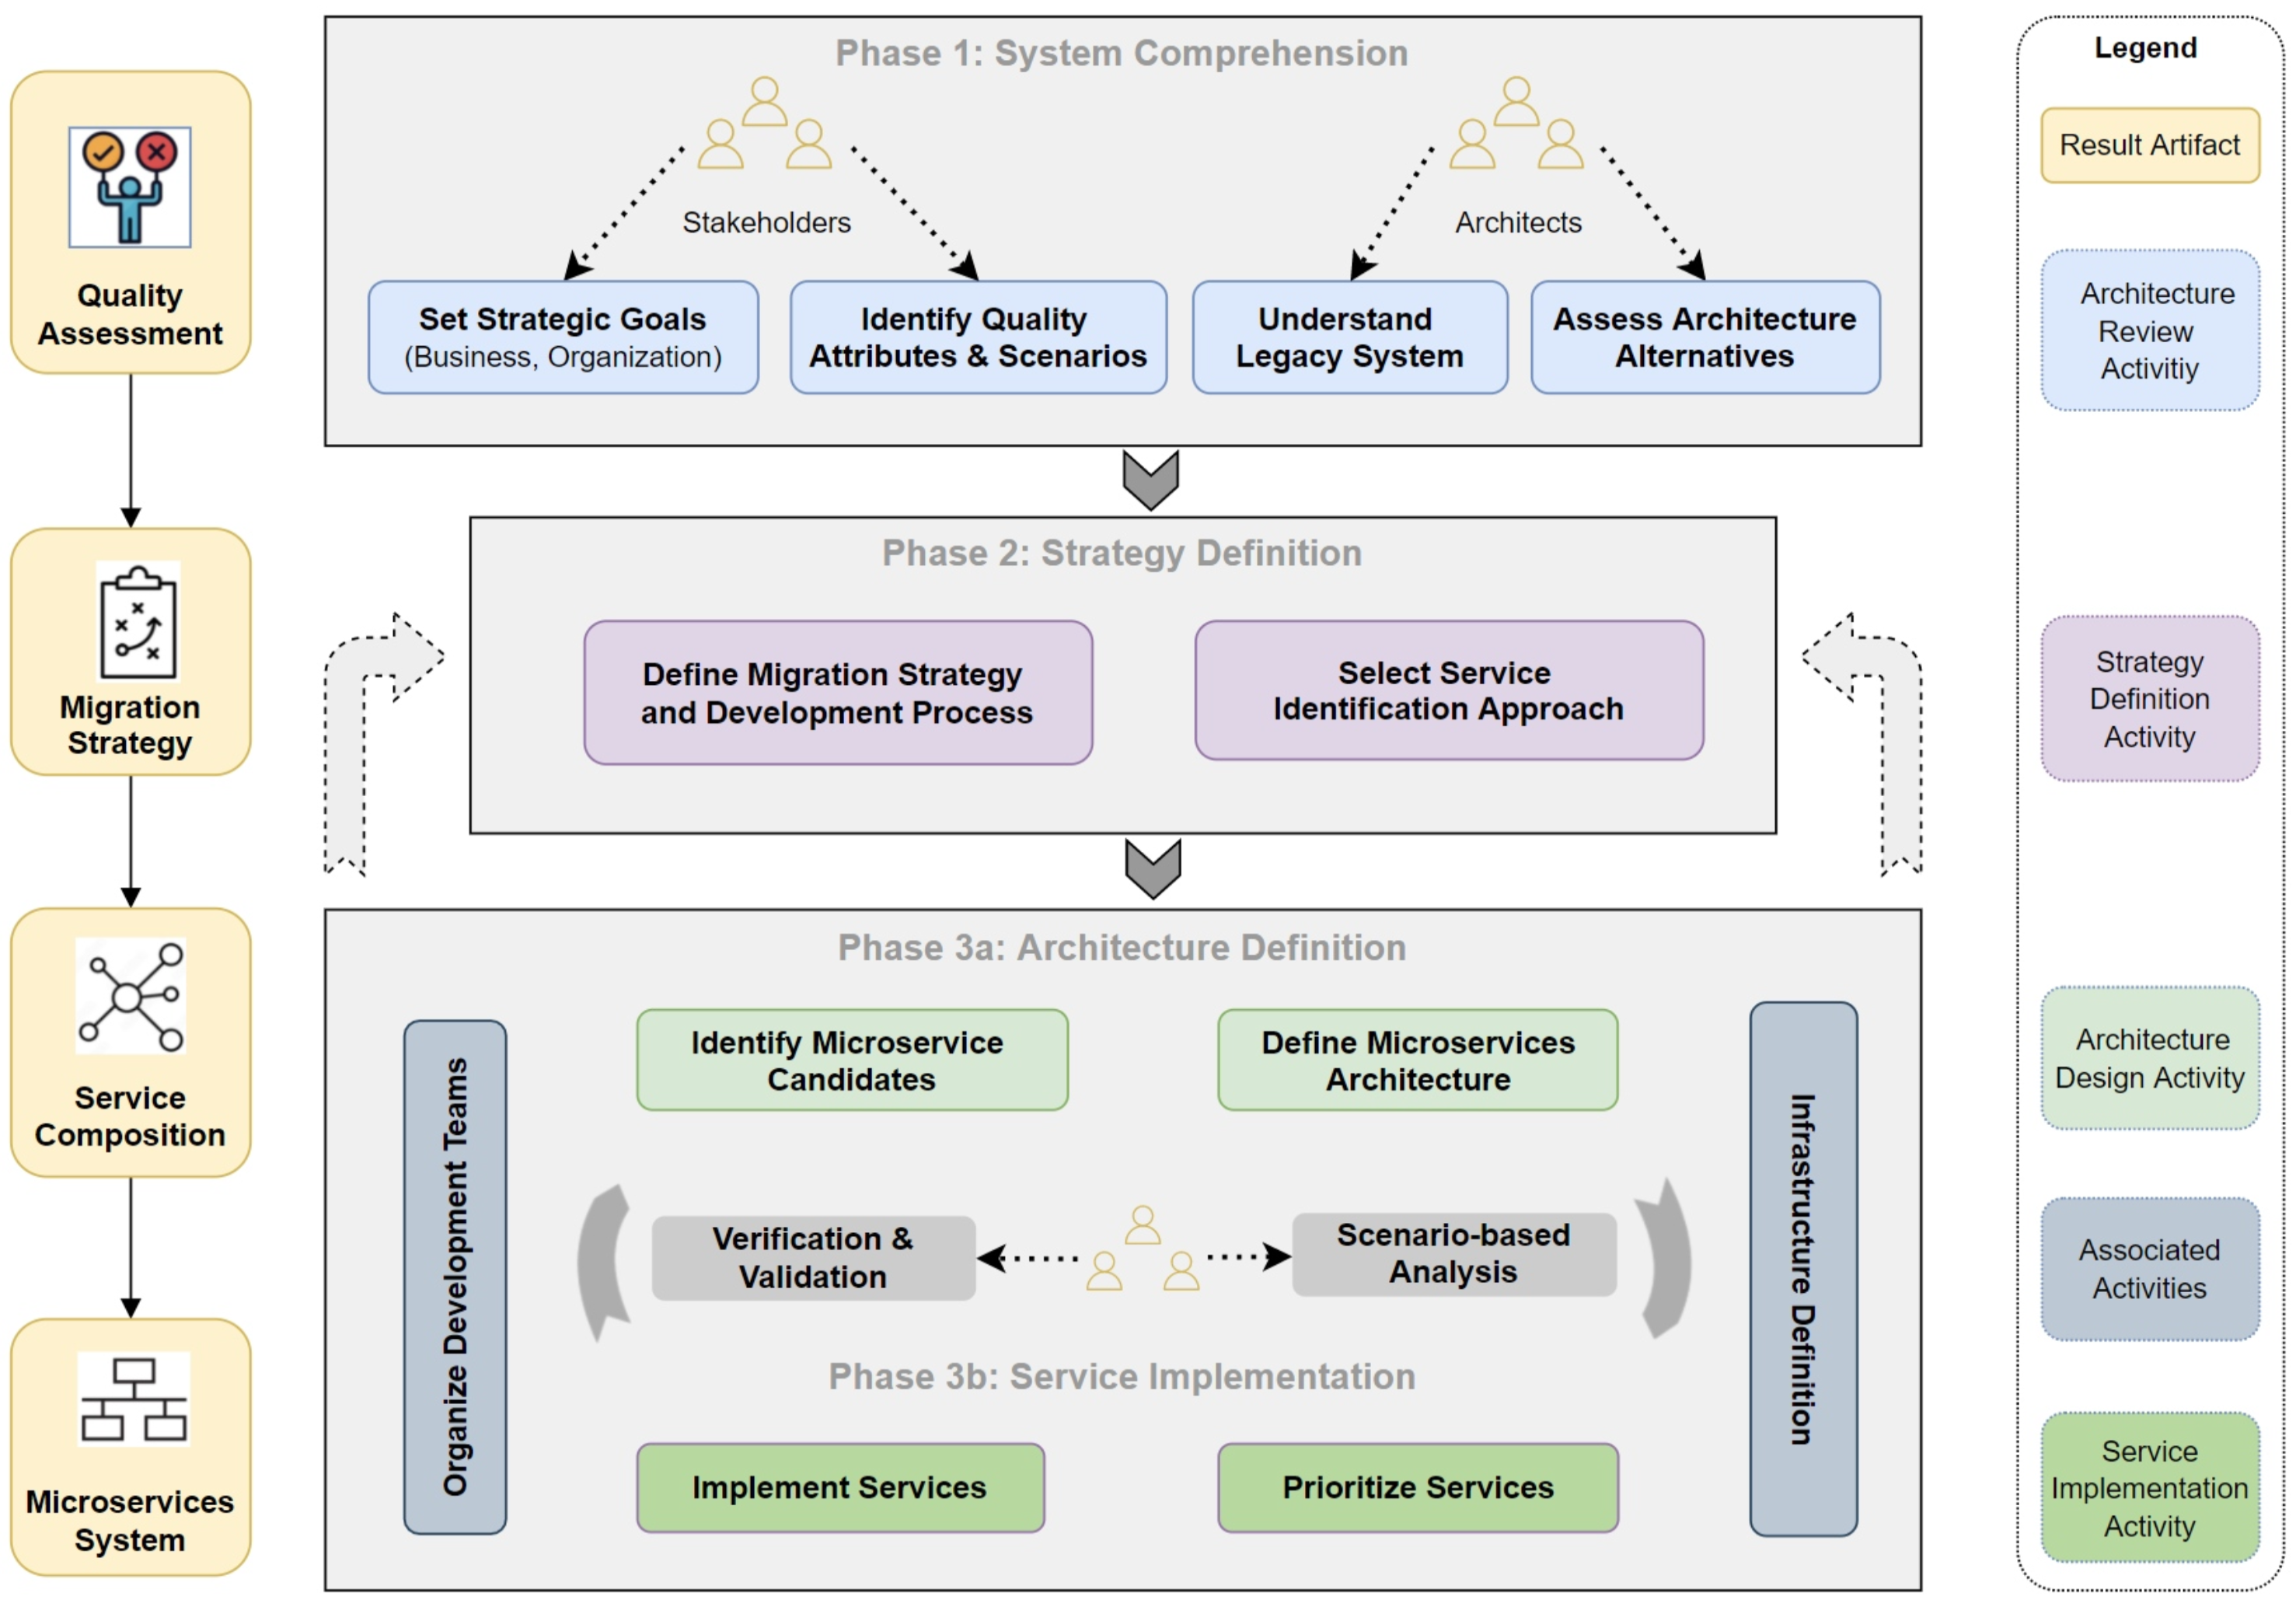
\includegraphics[width=\textwidth]{mmf-overview}
	\caption[Übersicht über \acrshort{mmf}]{
		Übersicht über das \gls{mmf} des \gls{ese} \cite{fritzsch2022architecturecentric}. Es sind die drei Phasen des Prozesses zu erkennen, sowie einige Schritte der einzelnen Phasen.
	}
	\label{fig:mmf-overview}
\end{figure}

\begin{itemize}
	\item \textbf{Phase 1: System Comprehension:}
	In Phase 1 wird das Verständnis des zu migrierenden Systems angestrebt.
	Mit den Stakeholdern werden dabei strategische Ziele für Produkt und Unternehmen definiert, sowie \glspl{qa} und gewünschte Szenarien identifiziert.
	Es sollen sich dadurch mögliche Treiber für die neue Microservices-Architektur herauskristallisieren.
	Durch das resultierende Verständnis des Systems wird ein Vergleich der alten monolithischen Architektur und einer potentiellen neuen Microservices-Architektur möglich.
	Architekten sollen dann mithilfe dieser Informationen eine Entscheidung für oder gegen die Migration zu Microservices fällen.
	Zum Zeitpunkt der Durchführung dieser Arbeit konnte im Tool nur die Eingabe der Szenarien mit den zugehörigen \glspl{qa} erfolgen.
	Die restlichen Schritte dieser Phase wurden erst nach Abschluss der Arbeit zum Tool hinzugefügt.
	\item \textbf{Phase 2: Strategy Definition:}
	Falls sich in Phase 1 für die Migration zu Microservices entschieden wurde, wird in Phase 2 die Planung der Migration begonnen.
	Die hauptsächliche Aufgabe in dieser Phase ist die Entscheidung, welche Migrationsstrategie benutzt werden soll, um das System zu modernisieren.
	Dafür kann zwischen (momentan) 115 verschiedenen Methoden gewählt werden, die aus akademischen Publikationen stammen.
	Das Tool kann Entwickler dabei unterstützen, indem es basierend auf Eingaben aus Phase 1 empfohlene Methoden vorschlägt.
	Einige dieser Methoden beinhalten die Nutzung von Tools, welche auch gesondert durchsucht werden können.
	Die verschiedenen Migrationsmethoden und Tools können von Admins importiert, exportiert und bearbeitet werden, wodurch die Erweiterung in zukünftigen Arbeiten vereinfacht möglich ist.
	\item \textbf{Phase 3a: Architecture Definition:}
	Phase 3 ist in zwei Teile aufgeteilt.
	Im ersten Abschnitt wird die neue Architektur definiert.
	Basierend auf der in der Planungsphase ausgewählten Methode zur Migration wird hier der \gls{sia} durchgeführt.
	Außerdem wird allgemeiner die Architektur des gesamten Systems geplant, wobei das Tool Entwickler durch eine Liste von vorgeschlagenen Patterns und Best Practices unterstützen kann.
	 Phase 3a und 3b sind eng verbunden, denn durch Erkenntnisse in der Implementierung kann die Planung häufig noch mehrmals überarbeitet werden und dadurch eine neue Iteration der Implementierung begonnen werden.
	\item \textbf{Phase 3b: Service Implementation:} In Phase 3b startet dann ein Zyklus von Im\-ple\-men\-tie\-rung\-en der in Phase 3a definierten Services.
	Bei Implementierung selbst kann das Tool Entwickler nicht unterstützen.
	Doch Bestandteil der Entwicklungszyklen ist auch, dass das entstehende System anhand der Qualitätsmerkmale zu bewerten.
	Dadurch kann eine unpassende Architekturdefinition oder auch eine unpassende Aufteilung in Services frühzeitig erkannt und korrigiert werden.
	Ist diese Phase abgeschlossen, ist eine erste Version des migrierten Systems fertig.
\end{itemize}

\section{jadice flow}

Das vorgestellte Framework wird in dieser Thesis nun erstmals zum Refactoring einer bereits vorhanden Microservices-Architektur in der Industrie benutzt.
Deswegen wird in diesem Abschnitt näher auf das Produkt \emph{jadice flow}\footnote{\url{https://www.levigo.de/jadice-flow/}} eingegangen, welches mit dem \gls{mmf} überarbeitet wird.

\jf ist ein Produkt der Firma \emph{levigo solutions}\footnote{\url{https://www.levigo.de/dokumentenmanagement/}}.
\emph{levigo solutions} beschäftigt über 30 Mitarbeiter, von denen ungefähr sechs seit vier Jahren an der Anwendung arbeiten.
\jf basiert bereits auf einer Microservices-Architektur, ist jedoch erst die erste Generation nach der Überführung des vorherigen Monolithen \emph{jadice server}\footnote{\url{https://www.levigo.de/jadice-server/}}.
Beide Produkte bieten workflowbasierte Dokumentenverarbeitung an, bei der mit komplexen Datenströmen umgegangen werden kann.
Durch den Umstieg auf eine Microservices-Architektur können in der neuen Generation einzelne Verarbeitungsschritte skaliert werden.
Der Großteil der Services ist in Java geschrieben, doch durch den Betrieb in Containern ist \jf prinzipiell unabhängig von der Programmiersprache.

Einen beispielhaften Workflow stellt der \emph{E-Mail converter} dar.
Dabei werden E-Mails in Einzelteile aufgeteilt (Körper, Anhänge) und diese dann einzeln in das Zielformat konvertiert.
Die einzelnen Arbeitsschritte dabei können parallelisiert und separat skaliert werden.
Am Ende werden die Ergebnisse kombiniert.
Im Gegensatz zu einfacher PDF-Darstellung von E-Mails in geläufigen Programmen bietet \jf zusätzliche Features, wie die tiefe Analyse und Darstellung von Archiven in Anhängen.

Da \emph{jadice flow} die erste Generation in Microservices-Architektur ist, wird noch ar­chi­tek­tu­relles Verbesserungspotential vermutet.
Durch die Analyse von \emph{jadice flow 1.0} mithilfe des Tools und weiterer Forschung im Rahmen dieser Bachelorarbeit sollte ein Refactoring-Prozess für \emph{jadice flow 2.0} angestoßen werden.

Obwohl das Framework ursprünglich für die Anwendung auf Monolithen gedacht ist, wird es in dieser Arbeit auf ein bereits migriertes System angewendet, um dessen Eigenschaften weiter zu verbessern.
Dadurch wird erforscht, inwiefern das Framework und das Tool für diesen Spezialfall einer bereits existierenden Microservices-Architektur geeignet sind.
Falls es deshalb für diesen Anwendungsfall zielführend gewesen wäre, hätte zusätzlich die ursprüngliche monolithische Anwendung von \jf (\emph{jadice server}) hinzugezogen werden können.
Die Ergebnisse dessen hätten dann mit \jf verglichen werden können.

\section{Ähnliche Forschung}

Aufgrund vieler Vorteile von Microservices vor allem direkt gegenüber traditionellen Monolithen (ausführlicher im \cref{sec:monolith-vs-microservices} diskutiert) ist die Migration zu Microservices zu einem großen Forschungsfeld geworden.
In diesem Abschnitt wird ein Überblick über für diese Arbeit relevante Publikationen gegeben.

\subsection{Grundlagen zum MMF}

Das Hauptuntersuchungsobjekt dieser Thesis sind das \gls{mmf} und der \gls{arh} des \gls{ese}.
Obwohl das Tool sich noch in einer prototypischen Phase befindet, wurde es bereits durch mehrere akademische Publikationen weiterentwickelt.
Im Folgenden wird ein Überblick über diese gegeben.
Im Jahr 2019 kategorisierten \Citet{10.1007/978-3-030-06019-0_10} zehn verschiedene Microservices-Migrationsmethoden.
Dabei wird ein Mangel an praktisch anwendbaren Methoden hervorgehoben, die gute Toolunterstützung und Metriken zur Verifikation der Ergebnisse bieten.
Als Folge darauf stellten \Citet{fritzsch2022architecturecentric} die Planung eines solchen Frameworks vor.
Der Migrationsprozess mit Framework und dessen Arbeitsweise in drei Phasen wird beschrieben.
Außerdem wird die Entwicklung eines Tools erwähnt, dass das Framework in Form einer webbasierten Lösung umsetzt und Entwickler bei der Migration unterstützt.
Die Entwicklung des Tools fand im Rahmen der Masterarbeiten von \Citet{master-tobias-haller} und \Citet{master-daniel-koch} statt.
\citeauthor{master-tobias-haller} forscht dabei an der erweiterbaren Speicherung von verschiedenen Migrationsmethoden und der Darstellung dieser in der Web-Applikation, dem \gls{arh}.
Damit wurde größtenteils das Backend und Phase 2 des Tools umgesetzt.
Schlussendlich wird außerdem eine empirische Bewertung des entstandenen Prototyps vorgenommen, die den Nutzen des Tools bestätigt und weiterführende Arbeit daran vorschlägt.
\Citet{master-daniel-koch} setzt die Arbeit an dem Tool fort, indem Phase 1 und 3 ergänzt werden.
Dabei wird viel an \glspl{qa} in der Migration zu Microservices geforscht.
Zu Beginn werden relevante \glspl{qa} gesammelt, wobei ein Großteil davon aus ISO 25010~\cite{ISO-25010} stammt.
Diese werden durch weitere, oft Microservices-kontextuelle \glspl{qa}, ergänzt.
Außerdem wird der Einfluss der \glspl{qa} auf Systemeigenschaften untersucht.
Eine weitere durchgeführte Untersuchung ist für den \gls{arh} ebenfalls sehr relevant.
Dabei wird gezeigt, wie \glspl{qa} genutzt werden können, um für die \glspl{qa} geeignete Migrationsverfahren sowie \bpp vorzuschlagen.
Die Ergebnisse wurden später verwendet, um die Suchfunktionen in Phase 2 und 3 des \gls{arh} auf Basis der vom Nutzer in Phase 1 definierten \glspl{qa} zu implementieren.

In 2023 führt \citeauthor{master-marvin-knodel} im Rahmen einer Masterarbeit \cite{master-marvin-knodel} eine erste Fallstudie zur Anwendung des \gls{mmf} durch.
Dabei wird das Framework im Ganzen als geeignet für die Migration im Einzelfall der Fallstudie bestätigt.
Außerdem werden kleinere Mängel hervorgehoben, die weitere Arbeit am Framework und Tool nahelegen.
Knodels Fallstudie unterscheidet sich von der in dieser Arbeit durchgeführten Fallstudie in einigen Punkten.
Zum einen bilden die Arbeiten verschiedene Anwendungsfälle ab.
Während in \Citet{master-marvin-knodel} der vermutlich gewöhnlichere Fall vorliegt, bei dem ein Monolith zu einer \gls{msa} umstrukturiert werden soll, fügt diese Arbeit einen neuen Anwendungsfall hinzu.
Die Evaluierung und Verbesserung einer bereits vorhandenen \gls{msa} erfordert möglicherweise andere Qualitäten des Frameworks, insbesondere bei der gezielten Suche nach Verfahren, die für diesen speziellen Fall überhaupt anwendbar sind.
Zum anderen steht eine weiter ausgeprägte Version des Tools \gls{arh} zur Verfügung.
Während die Suche nach Migrationsverfahren von in der Arbeit von \citeauthor{master-marvin-knodel} manuell ausgeführt wurde \cite{master-marvin-knodel}, kann zum Zeitpunkt dieser Arbeit die Suchfunktion des \gls{arh} dafür genutzt werden.

\subsection{Andere Frameworks}

Im Gegensatz zu den im nächsten Abschnitt behandelten Refactoringverfahren, die in großer Zahl akademisch publiziert wurden, liegt nur sehr wenig Forschung zu Verfahren auf der Metaebene vor \cite{on-a-metaprocess}.
Das Funktionsprinzip des \gls{mmf} ist dabei bisher einzigartig.
Wie auch \Citet{master-marvin-knodel} beschreibt, ist kein Framework bekannt, das den Vergleich und die Suche über viele konkrete Migrationsverfahren aus der Metaebene anbietet und damit direkt mit dem \gls{mmf} vergleichbar ist.
Es existieren nur wenige andere Frameworks, die im Gegensatz zu spezifischen Migrationsverfahren ebenfalls in der Metaebene Migrationsprozesse anleiten.
Jene sollen unter diesem Aspekt mit dem \gls{mmf} in Relation gesetzt werden.
%In diesem Abschnitt werden ähnliche Frameworks und Tools beschrieben, die Entwickler aus einer Meta-Perspektive bei der Migration unterstützen, wie es auch \gls{mmf}, beziehungsweise \gls{arh} machen.

\Citet{on-a-metaprocess} stellen die Methode \gls{m3k} vor, die auf dem OMG Essence Kernel~\cite{essence-kernel-omg} basiert.
Dieses Tool soll Ent\-wick\-ler\-teams beim Migrationvorgang helfen, indem ein allgemeiner Metaprozess definiert wird, der als Grundlage für spezifische Migrationsprozesse verwendet werden kann.
Die Evaluation von \gls{m3k} steht noch aus, Fallstudien und Expertenumfragen sind jedoch geplant.
Im Gegensatz zum \gls{mmf} liefert \gls{m3k} lediglich eine generische Prozessübersicht.
Verweise auf konkrete Methoden, um die einzelnen Schritte jedes Teils des Migrationsprozesses umzusetzen, sind dabei nicht vorhanden.
Nutzer werden dadurch bei der Umsetzung der identifizierten Schritte weniger unterstützt als beim \gls{mmf}.

%\Citet{software-architectural-migration-2021} stellen eine automatisierten Ansatz vor, mit dem Ar\-chi\-tek\-tur\-mi\-gra\-ti\-on\-en geplant werden können und der mehrere Zielarchitekturen neben Microservices unterstützt.
%Er basiert auf der formalen Modellierung der strukturellen und verhaltensbezogenen Aspekte der Architektur.
%Anhand dieser Eingaben werden Teile des Designs identifiziert, die überarbeitet werden sollten, wodurch eine neue Zielarchitektur bestimmt wird.
%Diese kann mit einer \emph{model-checking} Technologie formal gegenüber den funktionalen Anforderungen validiert werden.
%Mit einer KI-Planungstechnik werden einzelne Schritte für die Migration zur Zielarchitektur entworfen.
%Für diese Schritte können inkrementell vorläufige Modelle bestimmt werden, sowie formal überprüft werden, ob diese Modelle mit den definierten funktionalen und architektonischen Bedingungen übereinstimmen.
%Dieser Ansatz wurde mit fünf Architekturen von echten Software Systemen getestet, wobei unter anderem das Refactoring zu einer Microservices-Architektur erfolgreich war.
%In Zukunft soll die Liste der unterstützten Zielarchitekturen erweitert werden, sowie Unterstützung auf Implementierungs-Level hinzugefügt werden.

%In einem weiteren Artikel stellen \Citet{architect:a-framework} das Framework \emph{Architect} vor.
%Sie beschreiben, wie sie das System \emph{Artemis} mithilfe des Frameworks in zwei Phasen in eine Microservices-Architektur modernisieren.
%Während in der ersten Phase die Dekomposition des Systems durchgeführt wird, findet in der zweiten Phase die Trennung der geteilten Datenbank in mehrere Datenbanken nach \emph{database-per-microservice} Pattern statt.
%\emph{Architect} ist allerdings noch relativ limitiert, da es nur Projekte von Grund auf unterstützt, also keine Unterstützung für Software-Evolution bietet, nur dotnet-basierte Services erstellt und nur relationale Datenbanken unterstützt.

\subsection{Konkrete Refactoring-/Migrationsverfahren}

Im Gegensatz zu dem, was in dieser Arbeit bisher als \emph{Frameworks} bezeichnet wurde, werden in diesem Abschnitt konkrete Refactoring-Verfahren betrachtet.
Diese sind durch die Vorgabe einer spezifischen Strategie klar von Meta-Ansätzen wie dem \gls{mmf} abzugrenzen.
Der \gls{arh} speichert momentan 115 solcher Verfahren.
Ein wichtiges Feature des \gls{mmf} und \gls{arh} ist dabei die Kategorisierung dieser Verfahren, die eine individuelle Suche für verschiedene Nutzer des Frameworks mit unterschiedlichen Zielen ermöglicht.
Um einen Überblick über die Merkmale zu geben, in denen sich Methoden unterscheiden, werden folgend einige in akademischen Publikationen beschriebene Verfahren vorgestellt.

Eines der primären Merkmale ist das Ziel eines Verfahrens.
Die meisten Verfahren behandeln das Ziel, eine geeignete Dekomposition von Monolithen in Microservices zu finden, da dies eines der kompliziertesten Probleme bei der Migration darstellt.
Jene Verfahren sind für diese Thesis besonders relevant, da in der Forschungsfrage gezielt danach gesucht wird.
Beispiele für Methoden, die dieses Ziel verfolgen, sind \cite{arh-result-no-filter-3,arh-result-no-filter-2,arh-result-no-filter-5,arh-result-important-filter-4,arh-result-important-filter-7}.
Es gibt jedoch auch wenige andere Verfahren, die andere Ziele haben.
Dazu gehören die Prognose der Nützlichkeit einer potenziellen \gls{msa} für Systeme vor der Migration \cite{muP-a-dev-framework}, die Bewertung und Analyse von Schwachpunkten nach einer Migration \cite{https://doi.org/10.1002/spe.2974} oder die reine technische Umsetzung einer Dekomposition unter Angabe der erwünschten Service-Aufteilung \cite{arh-result-no-filter-4}.

Die für diese Thesis relevante Kategorie der Methoden, die der Dekomposition eines Monolithen dienen, kann anhand weiterer Merkmale unterteilt werden.
Dies umfasst hauptsächlich Merkmale, die die Funktionsweise der Verfahren betreffen.
Eine erste Unterscheidung kann bezüglich der Form der Eingabe in die Methoden gemacht werden.
Während einige mit Source-Code oder Laufzeit-Artefakten arbeiten und darauf statische und dynamische Analysen ausführen \cite{arh-result-no-filter-5}, erwarten andere Eingaben auf \acrlong{bp} Ebene \cite{arh-result-no-filter-3} oder \emph{User Stories} \cite{arh-result-no-filter-2}.

Die meisten Verfahren erstellen dann aufgrund dieser Eingaben einen Graphen mit verschiedenen atomaren Einheiten als Knoten.
Die Definition der atomaren Einheiten hängt dabei in der Regel von der Eingabe ab.
Anschließend wird bei verschiedenen Methoden mit unterschiedlichen Algorithmen versucht, eine bestmögliche Gruppierung in dem Graph zu finden.
Viele Verfahren verwenden unterschiedliche Versionen von \emph{Clustering}-Algorithmen \cite{arh-result-no-filter-3,arh-result-no-filter-5,arh-result-important-filter-4}, andere lösen das Problem mit evolutionären beziehungsweise genetischen Algorithmen \cite{arh-result-no-filter-2,arh-result-important-filter-7}.

Unter anderem abhängig von den Eingabemöglichkeiten gibt es verschiedene Stufen der Au\-to\-ma\-ti\-sie\-rung.
Vor allem Verfahren, die mit Code-Analysen arbeiten, sind teilweise voll-automatisiert \cite{Fil2023}.
Für andere Eingabearten wie \acrfull{bp} oder \emph{User Stories} ist höchsten semi-Automatisierung möglich, da diese Eingaben manuell erstellt werden müssen.
Die algorithmische Optimierung eines erzeugten Graphen ist in der Regel theoretisch automatisch möglich.
Allerdings ist dies nicht immer umgesetzt oder es wird lediglich auf mögliche Algorithmen für die Umsetzung verwiesen.


%Die wohl häufigste Art von Methoden sind solche, die Entwickler bei der Dekomposition von Monolithen in Microservices unterstützen.
%%Der \gls{arh} speichert momentan 20 dieser Werkzeuge.
%Jeder dieser Ansätze setzt unterschiedliche Bedingungen für die Anwendung voraus.
%Es gibt einige voll-automatische Werkzeuge, die zwar im Bezug auf die Eingabe unflexibler sind und damit nicht in jedem Fall anwendbar, aber eine einfachere und schnellere Anwendung ermöglichen.
%Auf der anderen Seite gibt es auch semi-automatische Werkzeuge, bei denen Entwickler oft über Formulare oder Graphen ihr System beschreiben müssen, da der Code nicht direkt analysiert werden kann.
%Dies bietet allerdings den Vorteil von höherer Kompatibilität.
%Im Folgenden werden zwei Bespiele für solche Werkzeuge vorgestellt.

%\Citet{Fil2023} stellen ein voll automatisiertes Migrationswerkzeug vor.
%Dieses arbeitet mit statischer Code-Analyse, um eine Graph-Repräsentation des monolithischen Systems zu erhalten.
%Ein solcher Graph dient als Ausgangslage für weitere automatische Analysen, die in mehreren Schritten eine Dekomposition in Services durchführen und diese weiter optimieren.
%Schlussendlich soll das Ergebnis eine Menge von hochgradig kohäsiven und lose gekoppelten Microservices sein.
%Dabei soll eine angemessene Granularität der Microservices erreicht werden.
%Die ebenfalls durchgeführte Evaluation ergibt positive Ergebnisse im Bezug auf Effektivität und Effizienz des Werkzeugs.
%Sie ist allerdings nur begrenzt valide, da nur wenige und kleine Monolithen als Eingabe für das Experiment fungiert haben.

%\Citet{PF4MD} stellen das semi-automatische Werkzeug \emph{PF4MD} vor, das Entwicklern bei der Dekomposition eines Monolithen in Microservices unterstützen soll.
%Sie beschreiben eine Ähnlichkeit der Microservices Architektur und der \gls{pf} nach \Citet{problem-frames} im Bezug auf das Aufteilen komplexer Probleme in kleinere, besser handlichere Teile.
%Aufgrund dieser Ähnlichkeit wollen sie das Problem der Dekomposition in Microservices mit der Beschreibung des Systems in graphisch umgesetzten Problem Diagrammen lösen, die auf \gls{pf} basieren.
%Mithilfe der eingegebenen Problem Diagramme und weiterer Eingaben, die die Problemkomplexität sowie die strukturelle Komplexität verschiedener Probleme quantifizieren, kann das Werkzeug eine Aufteilung der Probleme in verschiedene Gruppen vorschlagen.
%Eine Evaluation des Werkzeugs oder dieser Methode wurde bisher nicht durchgeführt.

%Eine weitere Art von Werkzeugen sind Werkzeuge für den Post-Migrationszeitraum.
%Diese unterstützen natürlich nicht die Migration, da diese schon abgeschlossen ist, sondern führen eine Bewertung des Ergebnisses durch und analysieren Schwachpunkte.
%Ein Beispiel zeigt der Artikel zur $\mu$TOSCA toolchain.
%\Citet{https://doi.org/10.1002/spe.2974} beschreiben, wie sie mit dem  $\mu$TOSCA Modell Architekturen von Microservices-basierten Systemen mit dem OASIS Standard TOSCA darstellen können.
%Außerdem beschreiben sie die Möglichkeit, das $\mu$TOSCA Modell eines Systems durch das zugehörige Kubernetes Deployment automatisch zu ermitteln.
%Das $\mu$TOSCA Modell einer Applikation soll dann dazu genutzt werden, potentielle architektonische Probleme zu finden.
%Für das Ermitteln des $\mu$TOSCA Modells und das Identifizieren von Architektur Smells stellen sie zwei Werkzeug Prototypen ($\mu$Miner und $\mu$Freshener) vor.

%Die letzte in dieser Arbeit behandelte Art von Werkzeugen sind Werkzeuge, die vor der Migration angewendet werden.
%Diese werden oft zur Prognose über eine mögliche Migration benutzt.
%Ein Beispiel dafür ist das von \Citet{muP-a-dev-framework} vorgeschlagene Framework $\mu P$.
%Dieses soll die Performance einer hypothetischen Microservices-Architektur durch das Design abschätzen können und dadurch Entwickler bei der Entscheidung unterstützen, ob sich eine Migration zu Microservices lohnt.
%Basierend auf vier Benchmarks wurde das Framework getestet, wobei der Fehler der Antwortzeiten konstant unter 10\% lag.

\chapter{Methodik}
\label{chap:methodik}

In diesem Kapitel wird der methodische Aufbau dieser Thesis beschrieben und begründet.
Die Arbeit ist als industrielle Fallstudie in Zusammenarbeit mit \emph{levigo solutions} konzipiert und dient der Evaluation des \gls{mmf} an einer bestehenden Microservices-Architektur.
Diese Fallstudie besteht aus zwei Hauptbestandteilen.
Im ersten Teil wird ein Refactoring des Produktes \emph{jadice flow} nach Anleitung des Frameworks durchgeführt.
Im zweiten Teil wird das Ergebnis dieses Refactorings verwendet, um eine Evaluation des Frameworks und Werkzeugs abzuschließen.

\section{Refactoring mit \gls{mmf}}

Die Vorgehensweise beim Refactoring ist durch das Framework sehr genau vorgegeben, daher wird das Refactoring in dieser Thesis in die gleichen drei Phasen unterteilt wie in \cref{sec:mmf} beschrieben.
In der ersten Phase wird ein Architekturreview nach \Citet{SVAHNBERG20071893} mit den Stakeholdern des Produkts durchgeführt.
Diese Methode wird in \cref{sec:methodik-architekturreview} näher beschrieben.
Das wesentliche Ergebnis dieses Reviews sind die gewünschten \glspl{qa} des Systems.
Diese Attribute sind die Basis für Phase 2 und 3 und werden in den \gls{arh} eingegeben. 
Dieser führt Berechnungen mit den \glspl{qa} durch und kann so eine Liste von Refactoring-Methoden vorschlagen, die nach ihrer Eignung für die \glspl{qa} sortiert sind.
Als weitere Eingabe dafür dienen bestimmte Filter, die in \cref{sec:durchführung-phase2} näher erläutert werden.
Aus der resultierenden Liste von Migrationsmethoden werden die besten Vorschläge betrachtet und bewertet, bevor einer davon ausgewählt und in den folgenden Phasen verwendet wird.
Analog dazu wird in Phase 3a eine sortierte Liste von Patterns und Best Practices vorgeschlagen, ebenfalls durch Eingabe von \glspl{qa} und Filtern.
Das Vorgehen bei der Auswahl der Filter sowie die spätere Inspektion der Vorschläge des \gls{arh} werden in Form von strukturierten Feldnotizen protokolliert.
Deren genauere Funktion und Form dieser wird folgend in \cref{sec:structured-field-notes} erläutert.

\subsection{Architekturreview}
\label{sec:methodik-architekturreview}

Das Architekturreview nach \Citet{SVAHNBERG20071893} basiert auf Szenarien-basierten Methoden, wie der \gls{saam} (\Citet{saam}) und der \gls{atam} (\Citet{kazman_2000}).
Das bedeutet, dass die gewünschten \glspl{qa} des Systems in Form von Szenarien erfasst und dokumentiert werden.
Dabei werden mit jedem Szenario zugehörige \glspl{qa} assoziiert, wodurch am Ende eine Abbildung aller \glspl{qa} auf ihre Priorität möglich ist.
Diese Abbildung ist das eigentliche Ergebnis, das der \gls{arh} als Eingabe für die weiteren Phasen benötigt.
Die Szenarien sind dabei lediglich ein Zwischenprodukt und sollen dabei helfen, eine genauere Vorstellung davon zu bekommen, welche spezifischen Situationen mit den \glspl{qa} verbunden sind.
Sie ermöglichen auch eine Bewertung der Wichtigkeit und technischen Schwierigkeit anhand konkreter Situationen, was bei abstrakten \glspl{qa} schwieriger wäre.

Um die wichtigsten Szenarien und \glspl{qa} zu ermitteln, haben \Citet{SVAHNBERG20071893} einen sechsschrittigen Plan entwickelt.
Diese sollen in einer etwa vierstündigen moderierten Gruppendiskussion mit den wichtigsten Stakeholdern des Produkts durchgeführt werden. 
Im ersten Schritt gibt der \gls{po} eine Einführung in das Projekt, in der Ziele für das Produkt sowie die Organisation geschildert werden.
Danach beginnt im Schritt 2 die Identifikation der \glspl{qa} in einer Brainstorming-Runde mit Beteiligung von \gls{po}, End-Nutzer und Architekten.
Die Liste der Qualitätskriterien gemäß ISO 9126~\cite{ISO-9126}\cite{ISO-9126-b} dient dabei als Vorlage für mögliche \glspl{qa}.
Im dritten Schritt ordnen \gls{po} und End-Nutzer die Liste der \glspl{qa} nach Wichtigkeit und fügen den drei wichtigsten jeweils zwei Szenarien hinzu.
Nach einer Pause präsentiert im vierten Schritt ein Softwarearchitekt die vorgeschlagene Architektur.
Anschließen werden im fünften Schritt die Szenarien nacheinander durchgegangen, analysiert und bewertet, inwiefern sie durch die Architektur erfüllt werden und wo etwaige Probleme bestehen.
Im sechsten Schritt werden alle festgestellten Probleme und Aspekte, die mehr Aufmerksamkeit benötigen, final diskutiert und der gesamte Prozess wird zusammengefasst.

Entgegen der eigentlichen Zielsetzung der Bewertung des Systems durch das Architekturreview nach \Citet{SVAHNBERG20071893} ist das Ziel des Reviews in dieser Thesis ein anderes.
Das gewünschte Ergebnis sind in diesem Fall lediglich die \glspl{qa} in Form von Szenarien, die in mit dem \gls{arh} verwendet werden können.
Die Schritte 4,5 und 6 werden daher nicht durchgeführt, da diese hauptsächlich der Bewertung des Systems unter den definierten \glspl{qa} dienen sollen.
Außerdem entfällt Schritt 1, da alle Teilnehmer des Architekturreviews bestens mit dem Produkt vertraut sind und schon einige Zeit daran arbeiten.
Somit bleiben im Wesentlichen nur noch Schritt 2 und 3 für diesen Anwendungsfall übrig.
Diese wurden zusätzlich noch weiter auf die Verwendung mit dem \gls{arh} angepasst.
Im Schritt 2 werden als Basis-\glspl{qa} statt der ISO 9126~\cite{ISO-9126} die von \Citet{master-daniel-koch} speziell für Microservices-Architekturen identifizierten \glspl{qa} (siehe \cref{fig:qas}) verwendet.
Dabei handelt es sich zu großen Teilen um die nach der Literaturrecherche wichtigsten \glspl{qa} aus der ISO 25010~\cite{ISO-25010}, die durch wenige Microservices-spezifische \glspl{qa} ergänzt wurden.
\begin{figure}
	\centering
	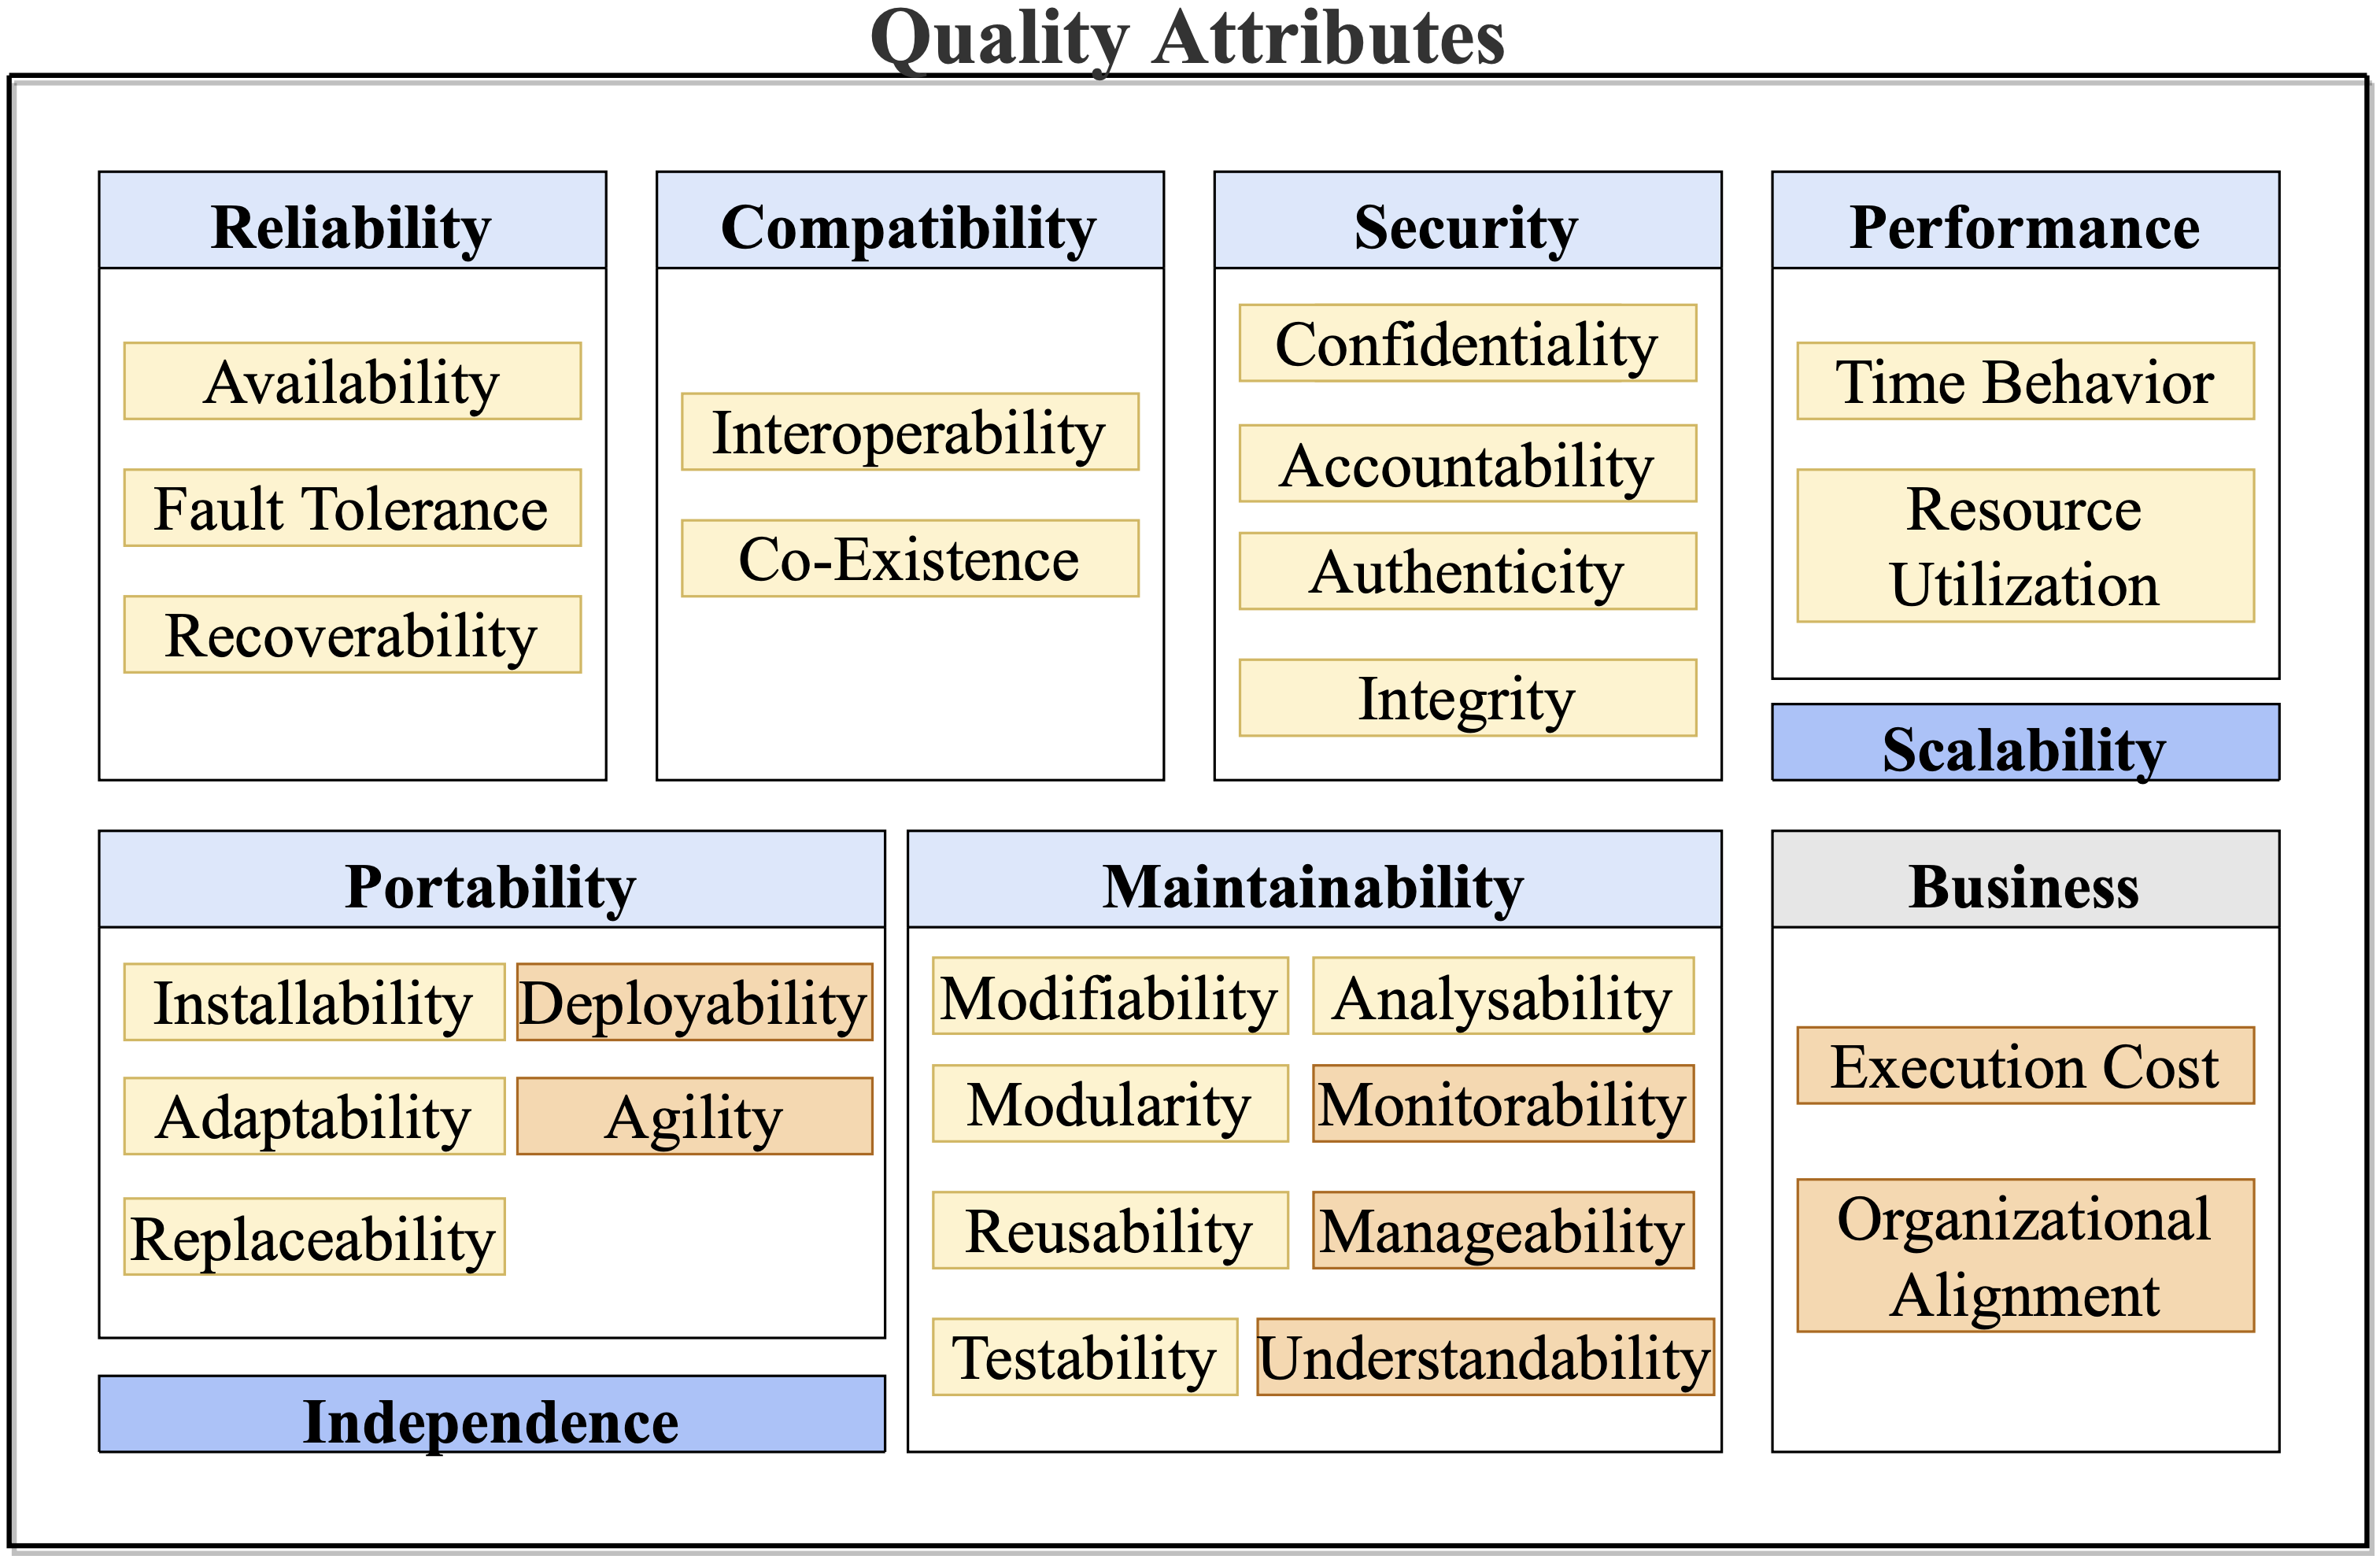
\includegraphics[width=\textwidth]{figures/qas}
	\caption[Spezielle \acrlongpl{qa} für Microservices-Architekturen]{
		Spezielle \acrfullpl{qa} für Microservices-Architekturen nach \Citet{master-daniel-koch}.
	}
	\label{fig:qas}
\end{figure}
Abgesehen davon, dass diese besser an die Architektur angepasst sind, ist es notwendig, diese zu verwenden, da der \gls{arh} nur diese zur Auswahl hat.
In der Vorlage von \Citet{SVAHNBERG20071893} war zwar keine vergleichbare explizite Bewertung oder Priorisierung der Szenarien gegeben.
Das ist allerdings aufgrund des Kontexts durch die qualitative Bewertung durch Menschen nicht nötig.
Im Vergleich dazu können bei der automatisierten Auswertung durch ein Werkzeug wie den \gls{arh} die Szenarien nicht automatisch eingeschätzt werden.
Aus diesem Grund erfolgt in Schritt 3 zusätzlich eine dreistufige Bewertung der Szenarien hinsichtlich ihrer Wichtigkeit und technische Schwierigkeit.
Die Bewertung erfolgt von A-C bewertet, wobei A für sehr wichtig und sehr technisch schwierig steht.

\subsection{Strukturierte Feldnotizen}
\label{sec:structured-field-notes}

Während Phase 1 also in einer Fokusgruppe durchgeführt wurde, findet die Bearbeitung in den folgenden Phasen größtenteils in Einzelarbeit statt.
Um dabei strukturiert zu protokollieren, welche Aktivitäten im Rahmen dieser Phasen durchgeführt wurden, werden systematisch durchgeführte Aktivitäten mit gemachten Erfahrungen und Herausforderungen dokumentiert und am Ende ausgewertet. 
Dazu werden strukturierte Feldnotizen verwendet~\cite{seaman2008qualitative}.
Dabei können die involvierten Stakeholder zur Rate gezogen werden.


\section{Evaluation des \gls{mmf}}

Das bis inklusive Phase 3a geplante Refactoring soll dann in Phase 3b im Rahmen eines minimalen Prototyps umgesetzt und simuliert werden, da ein Refactoring des kompletten Systems im zeitlichen Rahmen dieser Arbeit nicht möglich wäre.
Dabei entstehende Prototypen könnten Vorläufer von \emph{jadice flow 2.0} werden.

Im Nachgang sollen die Ergebnisse dieses Experiments ausgewertet werden. Um quantitativ vergleichbare Ergebnisse zu erhalten, sollen im Vorlauf des Experiments Vergleichskriterien und Messmethoden definiert werden, die es möglich machen, gleichartige Anwendungsfälle von \emph{jadice flow 1.0} und neuen Prototypen zu vergleichen.

\chapter{Anwendung des Frameworks auf jadice flow} % TODO reconsider chap name
\label{chap:anwendung}

In diesem Kapitel wird ein Architektur-Refactoring am Produkt \emph{jadice flow} geplant.
Dazu wird das \gls{mmf} benutzt, das in \cref{sec:mmf} beschrieben wird.
Unterteilt ist der Prozess in drei Phasen, deren Durchführung im Folgenden beschrieben wird.

\section{Phase 1 - Architekturreview}

In dieser Phase wird ein Architekturreview nach \Citet{SVAHNBERG20071893} durchgeführt.
Dabei handelt es sich um eine Architekturbewertungsmethode, die auf Szenarien-basierten Methoden wie \gls{saam} (\Citet{saam}) und \gls{atam} (\Citet{kazman_2000}) aufbaut.
Stakeholder definieren gemeinsam gewünschte Szenarien und ordnen diesen \glspl{qa} zu.
Außerdem wird den verschiedenen Szenarien jeweils ein Grad der Schwierigkeit und ein Grad der Wichtigkeit zugewiesen.
Die resultierenden Szenarien können in den \gls{arh} eingegeben werden.

Die Szenarien, die sich dabei im konkreten Fall zu \emph{jadice flow} ergeben haben, sind in Abbildung TODO zu sehen.

TODO nach Durchfürhung von Phase 1: 
 - Beschreibung der Szenarien und QAs
 - Explizite Änderungsvorschläge


\section{Phase 2 - Strategieplanung}
\section{Phase 3a - Architekturplanung}
\section{Herausforderungen bei der Durchführung}
%\section{Analyse der Ergebnisse}
%\section{Erstellung eines Refactoring-Konzepts}
%\subsection{Bestimmung der optimalen Granularität}
%\subsection{Optimierung des Kommunikationsmodells und der Verringerung des IO-Flaschenhalses}

\chapter{Erstellung der Prototypen}
\label{chap:erstellung_prototypen}

\chapter{Auswertung}
\label{chap:auswertung}

Die Auswertung dieser Fallstudie erfolgt mithilfe zwei verschiedener wissenschaftlicher Methoden.
Eine detaillierte Erläuterung der Methodik ist in \cref{chap:methodik} gegeben.
Zuerst werden in \cref{sec:auswertung-interviews} die durchgeführten Experteninterviews ausgewertet.
Außerdem werden in \cref{sec:auswertung-feldnotizen} die im Ver\-lauf der Anwendung des \gls{mmf} in dieser Thesis erstellten Feldnotizen analysiert.
Zum Abschluss dieses Kapitels werden die Ergebnisse dessen in \cref{sec:auswertung-diskussion} diskutiert und durch eine qualitative Bewertung des Refactoring-Prozesses durch den Autor ergänzt.

\section{Experteninterviews}
\label{sec:auswertung-interviews}

In diesem Abschnitt werden die Ergebnisse der Experteninterviews beschrieben und diskutiert.
Die Ex\-per\-ten\-inter\-views wurden mit dem Ziel durchgeführt, eine Evaluation der Anwendung des \gls{mmf}/\gls{arh} auf \jf von weiteren Personen zu erhalten, die nicht an der Durchführung beteiligt waren.
Die genaue Methodik der Interviews ist in \cref{sec:methodik-interviews} erläutert und der Leitfaden kann in \cref{chap:expert-interviews-leitfaden} gefunden werden.

Das erste Interview wurde gezielt mit dem \gls{po} von \jf durchgeführt.
Er begleitete alle Phasen der Thesis und benötigte deshalb keine thematische Einweisung.
Der \gls{po} hat die Präambel und das Informationsmaterial erst wenige Stunden vor dem Interview erhalten.
Durch die vorherige Mitarbeit des Teilnehmers an der Thesis konnte im ersten Interview zusätzlich evaluiert werden, ob die Verständnisfragen, inhaltlichen Fragen und der Zeitrahmen passend gewählt wurden.
Den anderen Teilnehmern, die nicht mit dem Inhalt der Thesis vertraut waren, wurden vier Tage vor den Interviews eine Präambel (\cref{chap:expert-interviews-preamble}) und fachliches Informationsmaterial (\cref{chap:expert-interviews-infobogen}) zur Verfügung gestellt.
Die Interviews konnten ohne größere Probleme oder Änderungen im Vergleich zur Planung durchgeführt werden.
Für jedes Interview wurde eine Stunde Zeit eingeplant, obwohl der Zeitaufwand auf 45 Minuten geschätzt worden war.
Die durchgeführten Interviews dauerten im Durchschnitt 50 Minuten.
Dadurch entstand kein Zeitdruck und die Teilnehmer mussten zu keinem Zeitpunkt in ihren Antworten unterbrochen werden.

Die Antworten der Teilnehmer wurden in \cref{fig:auswertung-interviews-kodierung} hinsichtlich der Nützlichkeit des \gls{arh} kodiert (Kodierleitfaden in \cref{fig:kodierleitfaden}).
Eine Übersicht über die drei interviewten Teilnehmer und deren Erfahrung ist in \cref{tab:expert-interviewees} zu finden.
\begin{table}[!ht]
  \centering
  \begin{tabular}{|l|l| p{1.8cm} p{1.5cm} p{2cm}|c|}
    \toprule
    \multirow{2}{*}[0cm]{\textbf{ID}} & \multirow{2}{*}[0cm]{\textbf{Rolle}} & \multicolumn{3}{c|}{\textbf{Erfahrung in Jahren}} & \textbf{An Thesis beteiligt} \\
     & & Software-entwicklung & Micro-services & \emph{jadice flow/ jadice server} & \\ \midrule
    \acrshort{po} & \acrlong{po} & \multicolumn{1}{c}{20} & \multicolumn{1}{c}{6} & \multicolumn{1}{c|}{13} & Ja \\
    \acrshort{sa} & \acrlong{sa}       & \multicolumn{1}{c}{13} & \multicolumn{1}{c}{7} & \multicolumn{1}{c|}{2} & Nein \\
   \acrshort{se} & \acrlong{se}     & \multicolumn{1}{c}{8} & \multicolumn{1}{c}{8} & \multicolumn{1}{c|}{6} & Nein \\
    \bottomrule
  \end{tabular}
  \caption[Teilnehmer der Experteninterviews]{
    Teilnehmer der Experteninterviews.
    An Thesis beteiligt bedeutet, dass der Teilnehmer an der Wahl der Migrationsverfahren beteiligt war.
    Der \acrshort{se} war ebenfalls an Phase 1 des \gls{mmf} beteiligt, das hat aber keine Relevanz für diese Interviews.
  }
  \label{tab:expert-interviewees}
\end{table}

In den folgenden Abschnitten werden die Ergebnisse dessen sowie explizierte und aggregierte Zusammenfassungen der Aussagen der Teilnehmer dar\-ge\-legt und diskutiert.

\begin{figure}%[!ht]
	\centering
	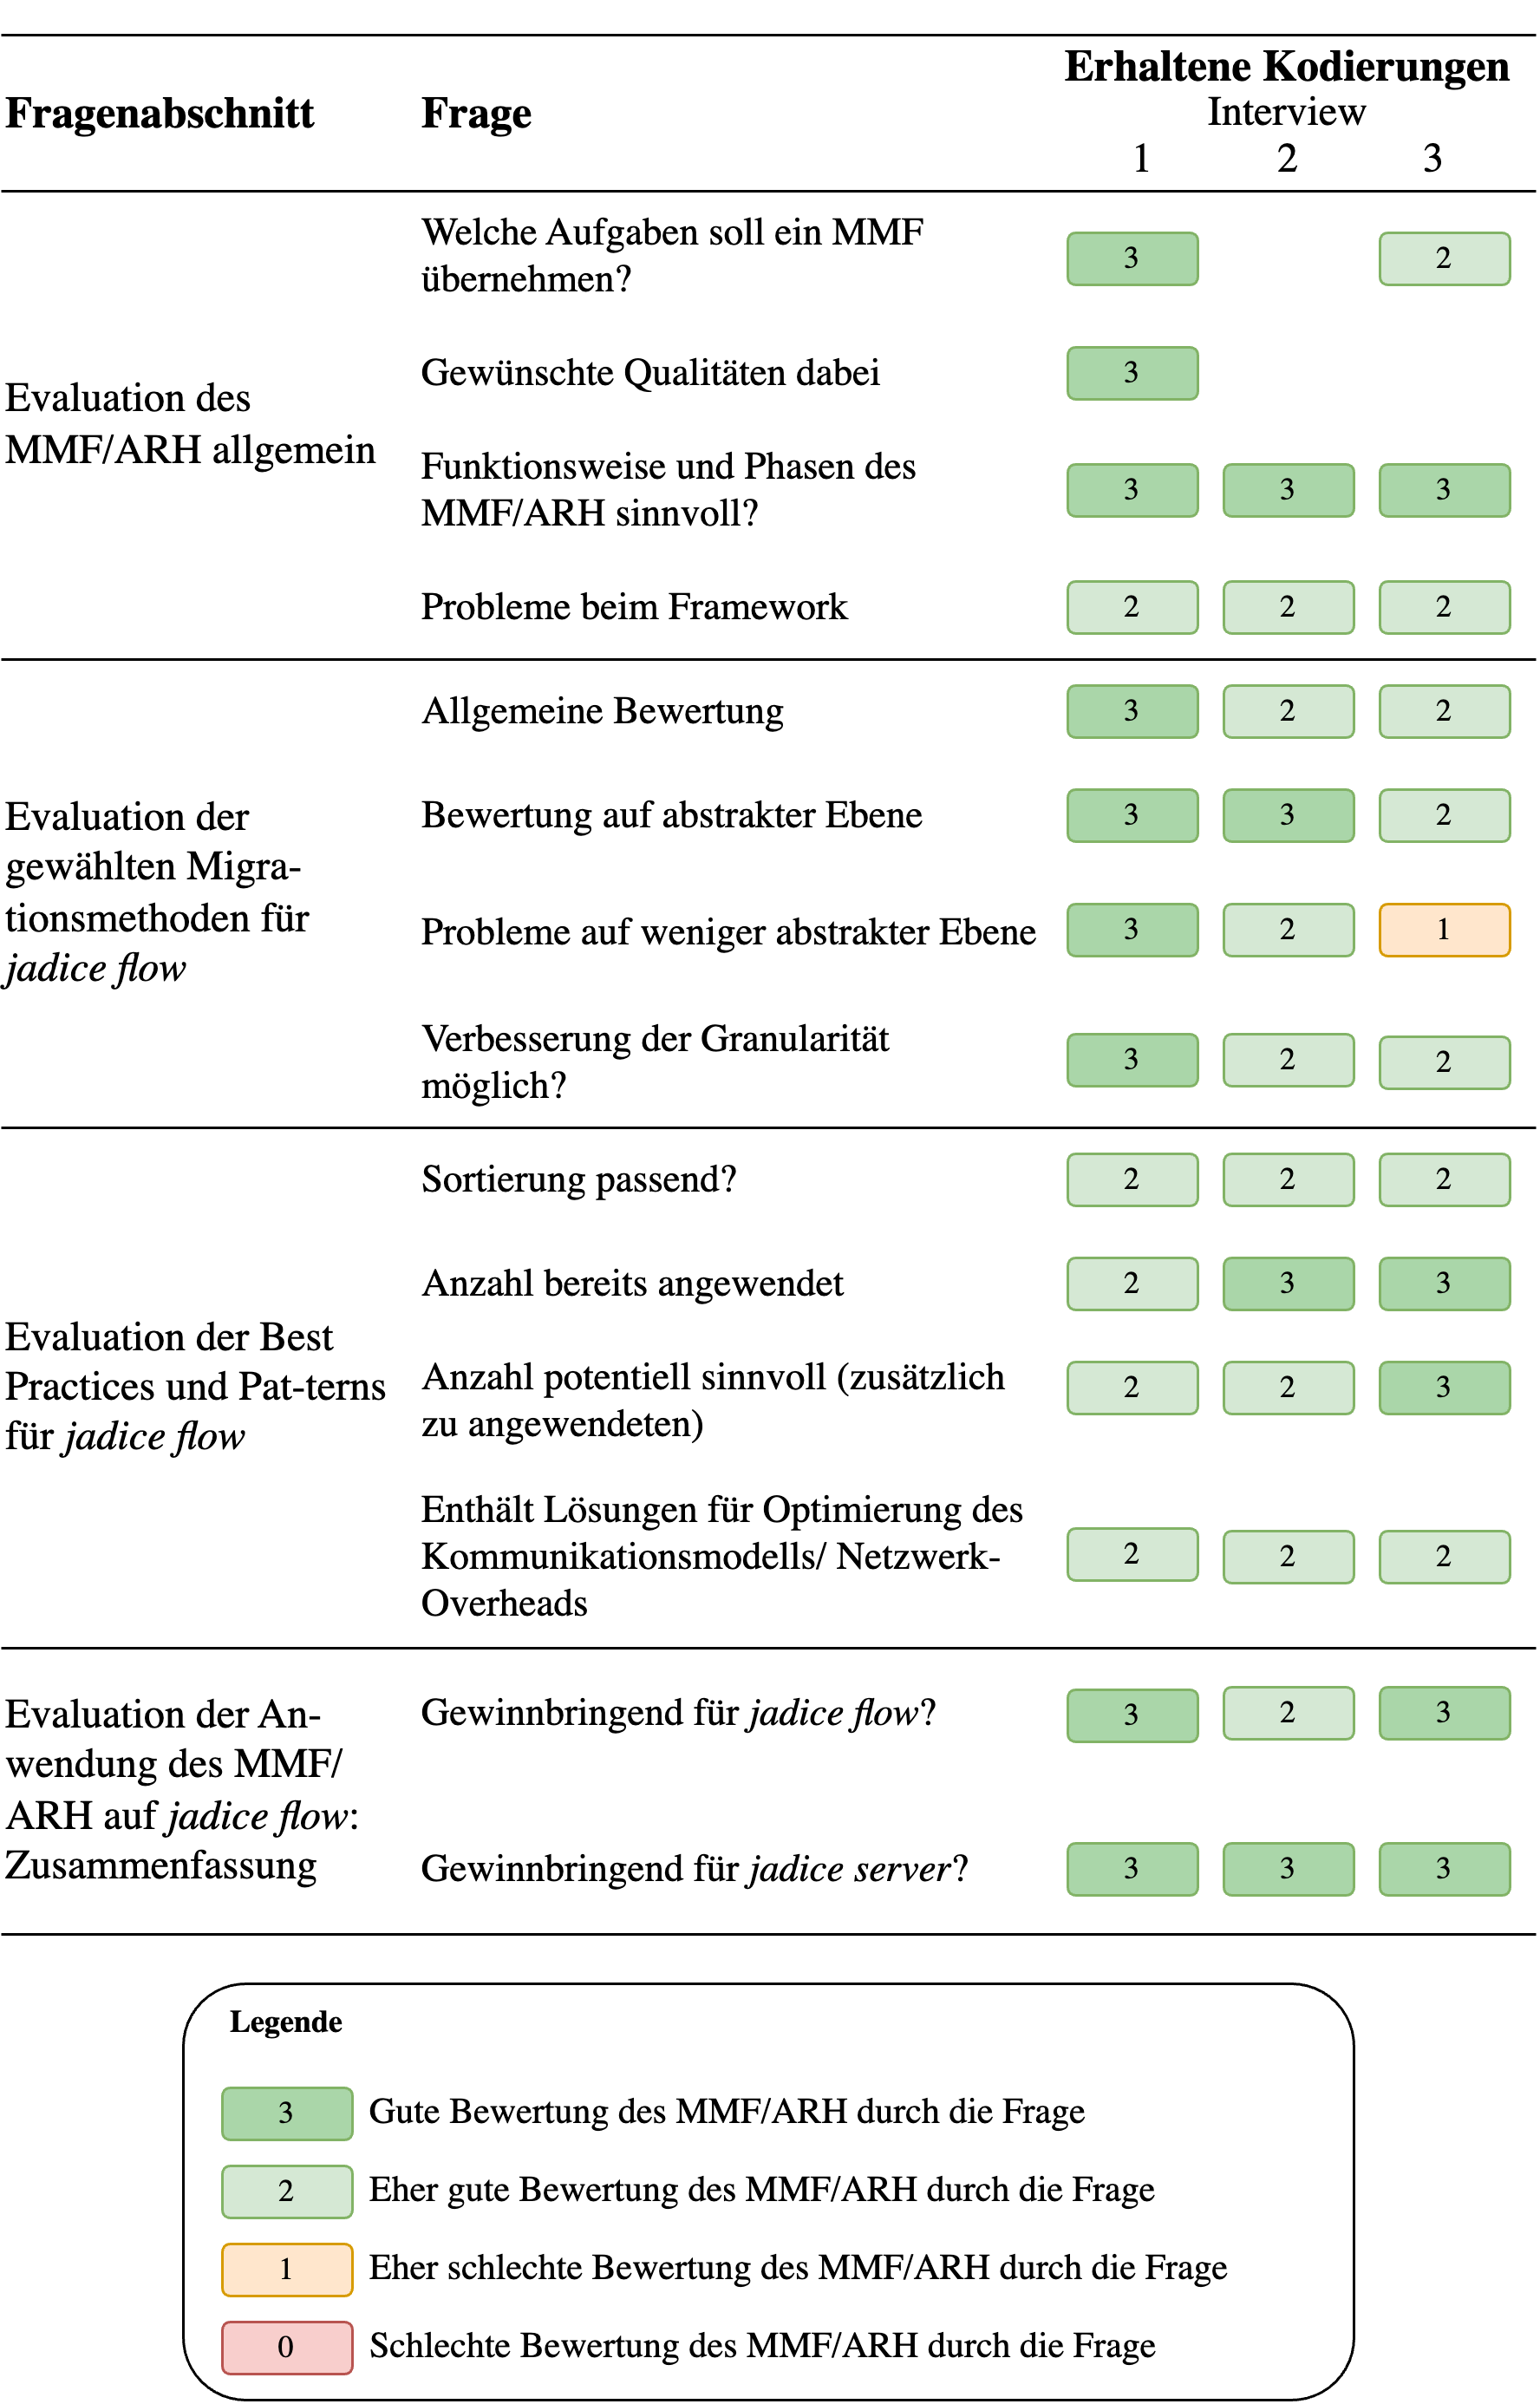
\includegraphics[width=0.8\textwidth]{interview-kodierung-auswertung.drawio}
	\caption[Auswertung Kodierung Experteninterviews]{
		Auswertung der Kodierung der Experteninterviews.
	}
	\label{fig:auswertung-interviews-kodierung}
\end{figure}
%Die Fragen der Interviews auf zwei Abschnitte unterteilt, deren Ergebnisse im Folgenden getrennt beschrieben werden.
%In \cref{sec:evaluation-mmf-allgemein} wird die Auswertung der Fragen, die sich auf die Evaluation des \gls{mmf}/\gls{arh} allgemein beziehen, vollzogen.
%Der hauptsächliche Teil der Auswertung findet dann in \cref{sec:evaluation-mmf-anwendung} statt, wo die spezifische Anwendung des Frameworks in Rahmen dieser Arbeit evaluiert wird.


\subsection{Evaluation des MMF/ARH allgemein}
\label{sec:evaluation-mmf-allgemein}

Dieser Teil der Interviews diente der allgemeinen Bewertung des Frameworks und des Tools.
Die Fragen wurden insbesondere ohne Bezug auf die in dieser Arbeit durchgeführte Migration gestellt.
Hierfür wurde ein Zeitrahmen von zehn Minuten vorgesehen, der mit durchschnittlich neun Minuten pro Interview auch eingehalten wurde.

\paragraph{Gewünschte Features eines \gls{mmf}:} In der ersten Frage sollte ohne Bezug zum \gls{mmf} oder \gls{arh} untersucht werden, welche Aufgaben ein \acrlong{mmf} allgemein für Entwickler bei der Migration von Monolithen zu Microservices übernehmen könnte.
Das Ziel ist es, die Antworten mit den tatsächlichen Funktionen des \gls{arh} abzugleichen und ggf. Ideen für zukünftige Funktionen des \gls{arh} zu sammeln.
In den Interviews hat sich herausgestellt, dass die Frage schwer verständlich ist, da zwei von drei Teilnehmern oft Konzepte eines Meta-Frameworks wie dem \gls{arh} mit konkreten Migrationsverfahren vermischt haben.
In einem Interview wurde daher die Frage schlussendlich übersprungen, da auch eine Wiederholung und Vertiefung der Frage keine Antwort erbrachte.
In nur einem Interview wurde die Frage hinreichend verstanden und beantwortet, um sinnvoll die damit verknüpfte zweite Frage stellen zu können.
Diese wurde in den anderen beiden Fällen schlicht übersprungen.

Zu großen Teilen wurden in den Antworten auf die erste Frage Funktionen genannt, die der \gls{arh} anbietet.
Dazu gehören das Sammeln von Informationen und die Definition von Anforderungen (umgesetzt in Phase 1)  sowie die Suche nach Verfahren, durch die primär die Granularität der Microservices optimiert werden kann (umgesetzt in Phase 2).
Als gewünschte Qualität wurde dabei genannt, dass eine große Auswahl an Verfahren bevorzugt wird, von denen dann mehrere manuell verglichen werden können.
Weitere Ideen sind die Visualisierung der gesammelten Informationen, ein Teilen der Informationen, um besser im Team arbeiten zu können und Tipps für den Migrationsprozess.
Letzteres könnte als teilweise umgesetzt bewertet werden, da das gesamte Framework als Leitfaden für die Migration gesehen werden kann.
Generell ist die Aussagekraft dieses Fragenabschnittes dadurch eingeschränkt, dass die Teilnehmer im Vorfeld über die Funktionsweise des \gls{arh} informiert wurden und somit diese Fragen nicht mehr völlig unbeeinflusst beantworten konnten.

\paragraph{Funktionsweise des \gls{mmf}:} Anschließend folgen Fragen zur Bewertung der generellen Funk\-ti\-ons\-wei\-se des \gls{mmf} in Phasen.
Alle Experten haben angegeben, dass sie die Phasenaufteilung als sinnvoll ansehen.
Die Durchführung einer Analyse des Systems und der Planung der Ziele in Phase 1 wurde als natürlicher Ausgangspunkt für allgemeine Refactoring-Prozesse wahrgenommen.
Vorschläge von Migrationsverfahren in der zweiten Phase wurden ebenfalls als positiv bewertet.
Es wird vermutet, dass so Verfahren gefunden werden können, die sonst nicht betrachtet worden wären.
Das Zusammenspiel der Phasen wurde ebenfalls als sinnvoll bewertet.
Es würde eine stetige Evaluierung der gewählten Vorgehensweise begünstigt und angestoßen werden.

\paragraph{Probleme des \gls{mmf}/\gls{arh}:} Auf die Frage nach Problemen am \gls{mmf} oder \gls{arh} wurden einige potentielle Probleme identifiziert.
Ein Teilnehmer kritisierte die Dokumentation des \gls{arh}.
Ein Beispiel dafür sei die Beschreibung der Filteroptionen für die Suche nach Migrationsverfahren.
Diese Kritik wurde vom Teilnehmer selbst direkt im Bezug auf das junge Entwicklungsstadium des Tools und die wissenschaftliche Orientierung relativiert.
Außerdem wurde von einem Experten hervorgehoben, dass der Haupteinflussfaktor auf die Nützlichkeit des Tools die verfügbare Datenbasis ist.
Diese müsse stetig aktualisiert und gut kategorisiert werden.
Eine weitere Kritik bezieht sich auf die Einschränkung auf bestimmte \glspl{qa} in der ersten Phase.
Da die verfügbaren \glspl{qa} auch in der Kategorisierung der Verfahren vorhanden sein müssen, ist das Modell nicht erweiterbar und bildet möglicherweise in bestimmten Anwendungsfällen nicht die nötigen Anforderungen ab.
Die Schwere dieser Kritiken wurde sowohl von den Teilnehmern als auch vom Autor als relativ gering eingeschätzt.

\subsection{Evaluation der Anwendung des MMF/ARH auf \jf}
\label{sec:evaluation-mmf-anwendung}

Während im ersten Teil der Fragen der Fokus auf der allgemeinen Funktionsweise des \gls{mmf} und \gls{arh} lag, wurde in diesem Teil ein Bezug zu der in dieser Arbeit durchgeführten Anwendung des Frameworks auf \jf hergestellt.
Dafür wurden erst Fragen zu zwei ausgewählten Migrationsmethoden und dann zu der Liste von \bpp, die der \gls{arh} für \jf anbietet, gestellt.
Als Hauptteil wurde in diesem Abschnitt der Interviews die größte Dauer vermutet, jedoch mit 20 Minuten trotzdem zu gering kalkuliert.
In nur einem Interview konnte diese Zeitspanne eingehalten werden, im Durchschnitt benötigte dieser Abschnitt 27 Minuten.
Vor allem die Befragung zu den \bpp dauerte mit durchschnittlich 14 Minuten länger als erwartet.
Durch das Einhalten des allgemeinen Zeitrahmens stellt das jedoch kein Problem dar.

\subsubsection{Evaluation der ausgewählten Migrationsmethoden für \jf}
\label{sec:evaluation-mmf-anwendung-methoden}

In diesem Fragenabschnitt wurden den Teilnehmern Fragen zu den ausgewählten Mi\-gra\-ti\-ons\-ver\-fah\-ren gestellt.
Diese wurden vor Beginn der ersten inhaltlichen Fragen im Rahmen der Verständnisfragen (siehe \cref{sec:verständnisfragen}) mit den Teilnehmern besprochen, um sicherzustellen, dass das Verständnis der Verfahren für eine Bewertung dieser ausreicht.
Im Folgenden werden die Verfahren auf Basis ihrer Reihenfolge im Informationsmaterial in \cref{chap:expert-interviews-infobogen} referenziert.
Verfahren 1 entspricht demnach \result{2} und Verfahren 2 \result{3}.
Als Einstieg dieses Teils wurde eine allgemeine Bewertung der Nützlichkeit der Verfahren im Bezug auf \jf abgefragt.
Oft wurden dadurch die folgenden Fragen zur Bewertung auf abstrakter und auf weniger abstrakter, technischer Ebene bereits teilweise beantwortet.

\paragraph{Abstrakte Funktionsweise:} Auf abstrakter Ebene wurden beide Verfahren von allen Teilnehmern als potentiell geeignet bewertet.
Vor allem die Art der Eingabe(n) und Ausgaben der Verfahren stand bei den Antworten im Fokus.
Ein Experte favorisierte das zweite vor dem ersten Verfahren, die anderen beiden umgekehrt.
Als Grund für die Bevorzugung des  zweiten Verfahrens wurde die besser passende Eingabe einer bereits vorhandenen \gls{msa} sowie die Visualisierung der Metriken für eine manuelle Überarbeitung der Architektur genannt.
Diese wird zusätzlich zur Optimierung der Serviceaufteilung mit einem Algorithmus, die auch das zweite Verfahren beinhaltet, angeboten.
Die anderen Experten bewerteten diese Vorteile des ersten Verfahrens als weniger wichtig und gaben an, dass sie die Eingabe in Form von einem \gls{bpmn}-Diagramm den User Stories vorziehen würden.
Das liegt vor allem daran, dass die User Stories eine weniger technische Ebene abbilden und damit schwerer greifbar ist, wie die Verbindung zwischen verschiedenen Einheiten analysiert und die Architektur verbessert werden soll.
Sie evaluierten die zweite Methode dennoch als potentiell sinnvoll anwendbar, nur eben als Ergänzung zur ersten Methode.

\paragraph{Technische Ebene:} Auf abstrakter Ebenen kann ein Konzept sinnvoll klingen und in der Realität trotzdem nicht funktionieren.
Deshalb wurde gefragt, ob die Experten sich konkrete Probleme bei der Umsetzung der Verfahren vorstellen können.
Hierbei muss beachtet werden, dass die Antwortmöglichkeiten der Experten bei der Frage sehr beschränkt sind, da sie die Verfahren nicht im Detail kennen.
Selbst bei besserer Informationslage über die Verfahren kann es passieren, dass bestimmte Probleme erst in der Praxis auffallen.
Die Evaluation dieser Frage soll deshalb nicht als Beweis für das sichere Gelingen der Verfahren in einer Anwendung mit \jf dienen, sondern nur beleuchten, ob die Verfahren schon bei anfänglicher Betrachtung Probleme aufwerfen, die den Versuch einer Anwendung infrage stellen.

Insgesamt wurden auf diese Frage wenige Probleme von den Experten genannt.
Ein Experte sah gar keine Probleme und konnte auf die kritische Nachfrage des Interviewers, der ein potentielles Problem benannte, sinnvoll argumentieren, dass er dieses nicht als Problem sieht.
Die anderen Experten nannten einige Probleme, von denen sie aber keines als zu kritisch für eine Anwendung der Verfahren einschätzten.
Unter anderem wurde für die Eingabe von \gls{bpmn}-Diagrammen argumentiert, dass man \glqq nur das bekommt, was man hereingibt\grqq{}.
Damit wird kritisiert, dass manuell erstellte Eingaben nicht objektiv sind und diese Subjektivität das Ergebnis beeinflussen kann.
Außerdem merkte ein anderer Experte allgemeiner an, dass nie komplett vollständige Eingabedaten vorliegen und durch fehlende Daten unvorhergesehene Probleme entstehen können.
Als Beispiel wurden \emph{Edge Cases} genannt, die womöglich nicht vom Verfahren berücksichtigt werden können, aber einen großen Einfluss auf den Erfolg einer Architektur haben können.

\paragraph{Bezug zur Forschungsfrage:} Abschließend zu den Verfahren wurde jeweils die Frage gestellt, ob summa summarum eine Anwendung der Verfahren als potentiell gewinnbringend im Bezug auf die Granularität der Microservices von \jf erachtet wird.
Da die Frage sehr hypothetisch ist, waren sich einige Teilnehmer etwas unsicher, insgesamt wurde aber von zwei Teilnehmern eine positive Tendenz verzeichnet und vom anderen Teilnehmer ein klares \glqq Ja\grqq{}.


\subsubsection{Evaluation der \bpp für \jf}
\label{sec:evaluation-mmf-anwendung-bp-patterns}

Als ebenfalls wichtiger Bestandteil des Frameworks wurde in den Interviews auch konkreter zur dritten Phase befragt.
Da im Gegensatz zu den Migrationsverfahren die Namen von \bpp in vielen Fällen genug Aussagekraft haben, damit die Teilnehmer das Konzept verstehen, wurde hier keine Vorselektion getroffen, sondern alle Einträge des \gls{arh} den Teilnehmern gezeigt.
Dabei ist klar, dass den Experten nicht alle Ansätze im Voraus bekannt sind oder durch den Namen klar werden.
Die einzige zeitlich sinnvolle Lösung dafür ist, alle nicht verstandenen \bpp zu ignorieren, was den Experten so auch gesagt wurde.
Das Ziel dieses Teils ist dabei die Bewertung der Experten, ob das Tool für Findung und Wahl von passenden \bpp zielführend ist und auch einen Vorteil gegenüber manueller Recherche bieten kann.

\paragraph{Ordnung der Ergebnisse:} Im ersten Schritt sollten die Experten die Sortierung der \bpp bewerten.
Dabei wurde hervorgehoben, dass diese auf Basis der \glspl{qa} \emph{Scalability}, \emph{Maintainability}, \emph{Performance} und \emph{Portability} entsteht.
Die Sortierung wurde grundlegend von allen Teilnehmern als sinnvoll bewertet.
An wenigen Stellen wurden Ergebnisse in einer anderen Priorisierung eingeschätzt, größtenteils wurden dabei aber Einwände wieder relativiert, nachdem erneut über die eingegebenen \glspl{qa} nachgedacht wurde.
Ein Teilnehmer erwähnte auch, dass man mit anderer Erwartungshaltung an diese Liste herangehen sollte als beispielsweise an die Liste der Migrationsverfahren.
Das liegt daran, dass sich nicht auf einzelne \bpp festgelegt werden muss, sondern mehrere kombinierbar sind.
Es wurde speziell hervorgehoben, dass auch zum Beispiel manche Ergebnisse mit nur einer Übereinstimmung gewinnbringend sein können, wenn sie für ein bestimmtes \gls{qa} sehr gut sind, aber kein anderes bedienen.

\paragraph{Bereits umgesetzte und potentiell sinnvolle \bpp:}
Als nächstes wurden die Einschätzungen der Experten zu der Anzahl der bereits in \jf umgesetzten \bpp sowie zu den noch nicht umgesetzten, aber potentiell sinnvollen, abgefragt.
Vom Interviewer wurde explizit angemerkt, dass lediglich eine Einschätzung abgegeben werden soll und Ergebnisse mit unbekannten Namen ignoriert werden sollen.
Im Durchschnitt wurde eingeschätzt, dass 13 Patterns und 15 Best Practices bereits in \jf (teilweise) umgesetzt sind und  5 Patterns sowie 4 Best Practices für die zukünftige Implementierung potentiell sinnvoll wären.
Die Abweichung der Antworten war dabei sehr hoch, vermutlich aufgrund der spekulativen Fragestellung.
Eine Einschätzung ist schwierig, wenn lediglich die Namen der Ergebnisse betrachtet werden.
Ein vorsichtiger Teilnehmer, der keine falschen Ergebnisse mit\-ein\-schließen will, könnte zu geringeren Zahlen kommen als ein selbstsicherer, optimistischer Teilnehmer.
Außerdem wurde die Anweisung, nur eine grobe Einschätzung abzugeben und nicht eine knapp 100 Ergebnisse lange Liste genau zu betrachten, unterschiedlich ernst genommen.
Dabei wurde beobachtet, dass der Teilnehmer mit der größten Abweichung deutlich schneller geantwortet hat.
Des Weiteren war bei diesen Antworten auffällig, dass in Prozentanteil von der Gesamtergebnisanzahl (beispielsweise \glqq 60\% der Patterns\grqq{}) geantwortet wurde statt in absoluten Zahlen.
Das könnte auf eine erhöhte Ungenauigkeit der Einschätzung dieses Teilnehmers hindeuten.

\paragraph{Bezug zur Forschungsfrage:} Abschließend wurde gefragt, ob eine Verbesserung des Kom\-mu\-ni\-ka\-ti\-ons\-mo\-dells beziehungsweise des Netzwerk-Overheads durch die \bpp der Liste für möglich gehalten wird.
Die Resonanz dabei war positiv, aber nicht übermäßig positiv.
Es wurden von den Experten jeweils ein bis zwei Möglichkeiten genannt, aber auch betont, dass die Zahl der dafür geeigneten Ergebnisse relativ gering ist und diese Ergebnisse in der Liste nicht hoch priorisiert sind.
Ein Experte erwähnte allerdings auch, dass die \glspl{qa} nicht unbedingt auf dieses Ziel ausgerichtet wurden und dadurch vermutlich diese Sortierung zustande kommt.

\subsubsection{Evaluation der Anwendung des \gls{mmf}/\gls{arh} auf \jf insgesamt}
\label{sec:evaluation-mmf-anwendung-insgesamt}

Zum Abschluss der Interviews wurden jeweils zwei Fragen gestellt, die die Ergebnisse aller vor\-he\-ri\-gen Fragen aggregieren sollten.
Es sollte insgesamt eingeschätzt werden, ob die Verwendung des Frameworks und des Tools zum momentanen Zeitpunkt gewinnbringend für \jf wäre.
Dieselbe Frage wurde anschließend im Bezug auf eine Verwendung des \gls{arh} in der Vergangenheit mit dem Vorgängerprodukt mit monolithischer Architektur wiederholt.

Zwei der Teilnehmer bewerteten die Verwendung zum jetzigen Zeitpunkt als sinnvoll.
Der andere Teilnehmer war unsicherer, tendierte jedoch auch dazu.
Alle waren sich darin einig, dass eine Anwendung für die Migration in der Vergangenheit noch wertvoller gewesen wäre.
Ein Experte war unsicher, ob die Verwendung des \gls{mmf} neues Optimierungspotenzial aufzeigt, das noch nicht bekannt ist.
Die Liste von \bpp sei zwar eine schöne Übersicht, aber wirklich neue Ansätze hätte er nicht gesehen.
Ein anderer Experte hob dagegen hervor, dass das Tool eine gute Übersicht für Architekten bietet und neue Anregungen fördert.
Bei diesen Meinungsverschiedenheiten der Experten konnte eine leichte Korrelation zwischen einer höheren Berufserfahrung der Experten und einer besseren Gesamtbewertung des Frameworks festgestellt werden.
Die Aussagekraft dieses Ergebnisses sollte aufgrund der geringen Teilnehmerzahl jedoch nicht überbewertet werden.

\section{Feldnotizen}
\label{sec:auswertung-feldnotizen}

Während der Anwendung des Frameworks auf \jf in dieser Arbeit wurden in den Phasen 2 und 3 strukturierte Feldnotizen erstellt, die wichtige Schritte dieser Phasen festhalten.
Die Methodik für die Erstellung der Feldnotizen ist in \cref{sec:structured-field-notes} beschrieben.
In diesem Abschnitt wird die Auswertung dieser Feldnotizen mit der in \cref{sec:methodik-auswertung-feldnotizen} erläuterten Codierung  durchgeführt.

Insgesamt wurden 18 Feldnotizen erstellt, wovon 14 in die zweite Phase und vier in die dritte Phase des \gls{mmf} fallen.
In Phase 1 wurden keine Feldnotizen formuliert.
Aufgrund der großen Anzahl von Feldnotizen in der zweiten Phase wurde die Phase für die Auswertung weiter in die übergeordneten Schritte \emph{Filterwahl} mit den \cref{feldnotiz:1,feldnotiz:2,feldnotiz:3} und \emph{Ergebnisbetrachtung} mit den \cref{feldnotiz:4,feldnotiz:5,feldnotiz:6,feldnotiz:7,feldnotiz:8,feldnotiz:9,feldnotiz:10,feldnotiz:11,feldnotiz:12,feldnotiz:13,feldnotiz:14} unterteilt.
Im Folgenden wird die Auswertung der zugehörigen Feldnotizen für jeden dieser Schritte beschrieben.

\subsection{Phase 2: Filterwahl}

In diesem Schritt wurden die Filter für die Suche nach Migrationsverfahren ausgewählt.
Die Entscheidungen dafür wurden ausschließlich in Besprechungen zwischen dem Autor und dem \gls{po} von \jf oder dem universitären Betreuer getroffen.
Dabei wurden drei Feldnotizen erstellt, deren Auswertung durch die festgelegte Kodierung in \cref{tab:auswertung-feldnotizen-1} zu sehen ist.

\begin{table}[!ht]
  \centering
  \begin{tabular}{m{2.8cm} | c c c | c}
    \toprule
    \multirow{2}{*}[0cm]{\textbf{Code}} & \multicolumn{3}{c|}{\textbf{Feldnotiz}} & \multirow{2}{*}[0cm]{\textbf{Summe} (3)} \\
     & \textbf{\fn{1}} & \textbf{\fn{2}} & \textbf{\fn{3}} & \\ \midrule
    Gut gelaufen                        & \checkmark & \checkmark & \checkmark & 3 (100\%)  \\ \hline
    Schlecht gelaufen                   & \checkmark &                       & & 1 (33\%)  \\ \hline
    Mehr gut gelaufen                   & \checkmark & \checkmark & \checkmark & 3 (100\%)  \\ \hline
    Mehr schlecht \:\:\:\:\:\: gelaufen & &                                  & & 0 (0\%)    \\ \hline
    Gutes Gefühl                        & & \checkmark & \checkmark            & 2 (67\%)   \\ \hline
    Schlechtes Gefühl                   & \checkmark & &                       & 1 (33\%)   \\
    Unsicherheit                        & \checkmark & &                       & 1 (33\%)   \\
    Frustration                         & & &                                  & 0 (0\%)    \\ \hline
    Verbesserungs\-vorschlag            & \checkmark & &                       & 1 (33\%)   \\ \hline
    Einzelarbeit                        & & &                                  & 0 (0\%)    \\ \hline
    Besprechung                         & \checkmark & \checkmark & \checkmark & 3 (100\%) \\
    \bottomrule
  \end{tabular}
  \caption[Auswertung Kodierung Feldnotizen Filterwahl]{
    Auswertung der Kodierung der Feldnotizen in Phase 2 beim übergeordneten Schritt \emph{Filterwahl}.
    Prozentuale Angaben hinter der Summe beziehen sich auf den Anteil des Auftreten des Codes zu der Anzahl der Feldnotizen.
  }
  \label{tab:auswertung-feldnotizen-1}
\end{table}


Wie in der Tabelle erkennbar ist, verlief dieser Schritt sehr positiv.
In jeder Feldnotiz wurde eine Sache vermerkt, die gut gelaufen ist und nur in einem Fall ein Problem.
Das ist auch an der Häufigkeit von 100 Prozent der Kodierung \glqq Mehr gut gelaufen\grqq{} zu sehen.

In den Einträgen der Empfindungen ist zu erkennen, dass trotz des positiven Verlaufs dieses Schritts einmal auch das schlechte Gefühl \glqq Unsicherheit\grqq{} festgehalten wurde.
Das hängt in diesem Fall jedoch nicht mit dem \gls{arh} oder der Migration zusammen, sondern wird auf die Unerfahrenheit des Autors mit der Anwendung der Methodik von Feldnotizen zurückgeführt.
Ansonsten wurde in 67 Prozent der Feldnotizen ein positives Gefühl vermerkt.
Zudem wurde ein Verbesserungsvorschlag kodiert, der direkt mit der Kodierung \glqq Schlecht gelaufen\grqq{} der \cref{feldnotiz:1} zusammenhängt.
Es wird die Beschreibung der Filteroptionen bemängelt.
Da der \gls{arh} noch in der Entwicklung ist, sind Mängel in der Dokumentation zu erwarten.

\subsection{Phase 2: Betrachtung der Filterergebnisse}

In diesem Schritt wurde mithilfe der im vorherigen Schritt gesammelten Filter eine Suche nach Migrationsverfahren durchgeführt.
Für jedes der acht in Einzelarbeit betrachteten Verfahren wurde je eine Feldnotiz erstellt.
Außerdem wurden drei Feldnotizen bei Besprechungen über die Bewertung der Verfahren für \jf erstellt.
Die Kodierung dieser ist in \cref{tab:auswertung-feldnotizen-2} zu sehen.

\begin{table}[!ht]
  \centering
  \begin{tabular}{m{2.8cm} | c c c c c c c c c c c | c}
    \toprule
    \multirow{2}{*}[0cm]{\textbf{Code}} & \multicolumn{11}{c|}{\textbf{Feldnotiz}} & \multirow{2}{*}[0cm]{\textbf{Summe} (11)} \\
     & \textbf{\fn{4}} & \textbf{\fn{5}} & \textbf{\fn{6}} & \textbf{\fn{7}} & \textbf{\fn{8}} & \textbf{\fn{9}} & \textbf{\fn{10}} & \textbf{\fn{11}} & \textbf{\fn{12}} & \textbf{\fn{13}} & \textbf{\fn{14}} & \\ \midrule
    Gut gelaufen                        & & \checkmark & \checkmark & \checkmark & & \checkmark & & \checkmark & \checkmark & \checkmark & \checkmark & 8 (73\%) \\ \hline
    Schlecht gelaufen                   & \checkmark & & & & \checkmark & \checkmark & \checkmark & & \checkmark & \checkmark & \checkmark            & 7 (64\%) \\ \hline
    Mehr gut gelaufen                   & & \checkmark & \checkmark & \checkmark & & & & \checkmark & & &                                             & 4 (36\%) \\ \hline
    Mehr schlecht \:\:\:\:\:\: gelaufen & \checkmark & & & & \checkmark & & & & & &                                                                   & 2 (18\%) \\ \hline
    Gutes Gefühl                        & & \checkmark & \checkmark & & & & & & & &                                                                   & 2 (18\%) \\ \hline
    Schlechtes Gefühl                   & \checkmark & & & & & & & & & & \checkmark                                                                   & 2 (18\%) \\
    Unsicherheit                        & & & & & & & & & & & \checkmark                                                                              & 1 (09\%) \\
    Frustration                         & \checkmark & & & & & & & & & &                                                                              & 1 (09\%) \\ \hline
    Verbesserungs\-vorschlag            & \checkmark & & & & & & & & & &                                                                              & 1 (09\%) \\ \hline
    Einzelarbeit                        & \checkmark & \checkmark & \checkmark & & \checkmark & \checkmark & \checkmark & & \checkmark & \checkmark & & 8 (73\%) \\ \hline
    Besprechung                         & & & & \checkmark & & & & \checkmark & & & \checkmark                                                        & 3 (27\%) \\
    \bottomrule
  \end{tabular}
  \caption[Auswertung Kodierung Feldnotizen Ergebnisbetrachtung]{
    Auswertung der Kodierung der Feldnotizen in Phase 2 beim übergeordneten Schritt \emph{Ergebnisbetrachtung}.
    Prozentuale Angaben hinter der Summe beziehen sich auf den Anteil des Auftreten des Codes zu der Anzahl der Feldnotizen.
  }
  \label{tab:auswertung-feldnotizen-2}
\end{table}


Die Ergebnisse dieses Schritts fallen gemischt aus.
In 73 Prozent der Feldnotizen wurden positive Aspekte notiert, jedoch wurden in fast genauso vielen Feldnotizen (64 Prozent) auch negative Aspekte festgehalten.
Durch \glqq Gut gelaufen\grqq{} und \glqq Schlecht gelaufen\grqq{} wurde in diesem Schritt bei der Ergebnisbetrachtung der Eindruck von dem jeweiligen Verfahren kodiert.
Bei nur zwei der Feldnotizen der Ergebnisbetrachtung in Einzelarbeit wurde \glqq Gut gelaufen\grqq{} kodiert, ohne dass \glqq Schlecht gelaufen\grqq{} kodiert wurde.
Diese beiden Verfahren wurden für die Phase 3 ausgewählt.
Letztendlich wurde jedoch doppelt so oft \glqq Mehr gut gelaufen\grqq{} kodiert wie \glqq Mehr schlecht gelaufen\grqq{}.
Der Schritt kann daher trotz gewisser Schwierigkeiten als größtenteils positiv verlaufen interpretiert werden.
In den Besprechungen wurde früh festgestellt, dass die Ergebnisse Optionen enthalten, deren Anwendung potentiell möglich ist.
Das spiegelt sich auch darin wider, dass in 67 Prozent der Besprechungen mehr gut gelaufen ist und nur in einem Fall gleich viel gut wie schlecht gelaufen ist.
Die große Anzahl der Kodierungen von \glqq Schlecht gelaufen\grqq{} hängt größtenteils mit Verfahren zusammen, die sich weniger gut für die Anwendung an \jf eignen.
Jedoch ist auch von anderen Suchmaschinen bekannt, dass nicht alle Suchergebnisse zur Vorstellung des Suchenden passen.
In der Praxis wird sich jedoch vermutlich zeigen, dass es genügt, ein bis zwei passende Verfahren mit \gls{arh} zu finden zu und diese zu verwenden.
Eine größere Auswahl an passenden Verfahren wäre dennoch wünschenswert.
Allerdings ist es aufgrund des frühen Stadiums des \gls{arh} wahrscheinlich, dass die Auswahl an Verfahren in Zukunft noch erweitert wird.
Außerdem bildet die durchgeführte Suche nur die Kriterien ab, die für \jf als sinnvoll befunden wurden.
Die Anzahl der sinnvollen Ergebnisse kann für andere Anwendungsfälle variieren.

Die in diesem Schritt notierten Gefühle sind relativ neutral.
In der ersten Feldnotiz (\cref{feldnotiz:4}) wurde Frustration vermerkt, da das erste Suchergebnis, für welches der \gls{arh} mit Abstand die größte Übereinstimmung angezeigt hat, als ungeeignet befunden wurde.
In der letzten Feldnotiz (\cref{feldnotiz:14}) wurde vermerkt, dass es Unsicherheiten bezüglich der zeitlichen Umsetzbarkeit der beiden ausgewählten Verfahren gibt.
Diese Gefühle überwiegen aber nicht den verzeichneten positiven Gefühlen bei der Betrachtung der zwei favorisierten Verfahren in \cref{feldnotiz:5,feldnotiz:6}.

Der in \cref{feldnotiz:4} notierte Verbesserungsvorschlag bezieht sich auf die Frustration in dieser Feldnotiz.
Es wird vorgeschlagen, eine Filteroption zu implementieren, um unpassende Ergebnisse auszuschließen.

\subsection{Phase 3: Anwendung der Migrationsverfahren}
\label{sec:feldnotizen-auswertung-phase3}

In der dritten Phase des \gls{mmf} wurden lediglich vier Feldnotizen erstellt, da nur ein kleiner Teil der Phase durchgeführt wurde.
Die Umsetzung der Phase 3b wurde frühzeitig ausgeschlossen.
Der Hauptteil der Phase 3a, welcher die Anwendung eines Migrationsverfahrens beinhaltet, konnte aufgrund der zeitlichen Beschränkung einer Thesis und Problemen mit den Verfahren nur teilweise durchgeführt werden.
Da in dieser Thesis nicht bis zur Planung einer neuen Architektur fortgeschritten wurde, fand auch keine Wahl von \bpp statt.

Die vier vorhandenen Feldnotizen beschreiben den Versuch, die beiden als Favoriten identifizierten Migrationsverfahren anzuwenden.
Wie in \cref{tab:auswertung-feldnotizen-3} zu sehen ist, war dieser Versuch nicht erfolgreich.
\begin{table}[!ht]
  \centering
  \begin{tabular}{m{2.8cm} | c c c c | c}
    \toprule
    \multirow{2}{*}[0cm]{\textbf{Code}} & \multicolumn{4}{c|}{\textbf{Feldnotiz}} & \multirow{2}{*}[0cm]{\textbf{Summe} (4)} \\
     & \textbf{\fn{15}} & \textbf{\fn{16}} & \textbf{\fn{17}} & \textbf{\fn{18}} & \\ \midrule
    Gut gelaufen                        &  & \checkmark &  &                                & 1 (25\%)  \\ \hline
    Schlecht gelaufen                   & \checkmark & \checkmark & \checkmark & \checkmark & 4 (100\%) \\ \hline
    Mehr gut gelaufen                   &  &  &  &                                          & 0 (0\%)   \\ \hline
    Mehr schlecht \:\:\:\:\:\: gelaufen & \checkmark & \checkmark & \checkmark & \checkmark & 3 (75\%)  \\ \hline
    Gutes Gefühl                        &  &  &  &                                          & 0 (0\%)   \\ \hline
    Schlechtes Gefühl                   & \checkmark & \checkmark & \checkmark & \checkmark & 4 (100\%) \\
    Unsicherheit                        &  & \checkmark &  &                                & 1 (25\%)  \\
    Frustration                         & \checkmark &  & \checkmark & \checkmark           & 3 (75\%)  \\ \hline
    Verbesserungs\-vorschlag            &  &  &  &                                          & 0 (0\%)   \\ \hline
    Einzelarbeit                        & \checkmark & \checkmark & \checkmark &            & 3 (75\%)  \\ \hline
    Besprechung                         &  &  &  & \checkmark                               & 1 (25\%)  \\
    \bottomrule
  \end{tabular}
  \caption[Auswertung Kodierung Feldnotizen Methodenanwendung]{
    Auswertung der Kodierung der Feldnotizen in Phase 3 beim übergeordneten Schritt \emph{Methodenanwendung}.
    Prozentuale Angaben hinter der Summe beziehen sich auf den Anteil des Auftreten des Codes zu der Anzahl der Feldnotizen.
  }
  \label{tab:auswertung-feldnotizen-3}
\end{table}

In nur einer Feldnotiz wurde etwas notiert, das gut gelaufen ist.
Dagegen ist in allen Feldnotizen etwas schlecht gelaufen.
75 Prozent der Notizen wurden mit \glqq Mehr schlecht gelaufen\grqq{} bewertet.
Jede Notiz enthielt ein negatives Gefühl, dreimal Frustration und einmal Unsicherheit.
Ein positives Gefühl wurde nie vermerkt.

Die schlechten Ergebnisse in dieser Phase sind hauptsächlich auf Zeitgründe und die Schwierigkeit bei der Umsetzung der ausgewählten Migrationsverfahren zurückzuführen.
Eine detailliertere Beschreibung der Probleme ist in \cref{sec:anwendung-verfahren} gegeben.
Für die Probleme werden hauptsächlich zwei Quellen vermutet.
Zum einen wurden die Verfahren nur von einer Person im Detail betrachtet und versucht umzusetzen.
Diese Person ist relativ unerfahren, was das Verständnis von wissenschaftlichen Artikeln mit komplexen Algorithmen und Formeln einschränken könnte.
Auf der anderen Seite sind bestimmte Details, zumindest im zweiten Verfahren, wenig ausführlich oder gar nicht beschrieben.
Für eine erfolgreiche Umsetzung dieses Verfahrens wird ein hoher Eigenentwicklungsaufwand eingeschätzt, um den Algorithmus und enthaltene Formeln zu verstehen und umzusetzen.

\subsection{Überblick über die Feldnotizen}

Nachdem die Ergebnisse der Auswertung der Feldnotizen pro Phase beziehungsweise Schritt in einzelnen Abschnitten beschrieben wurden, erfolgt in diesem Abschnitt eine Betrachtung der Ergebnisse der Feldnotizen aus übergeordneter Perspektive.
Für jeden übergeordneten Schritt wurde die Summe der Kodierung aller enthaltenen Feldnotizen zusammen in der \cref{tab:auswertung-feldnotizen} visualisiert.
\begin{table}[!ht]
  \centering
  \begin{tabular}{m{2.8cm} | M{1cm} m{0.3cm} M{1.8cm} m{0.3cm} M{1.9cm} m{0.3cm} p{0cm} | M{1.8cm}}
    \toprule
    \multirow{2}{*}[-0.3cm]{\textbf{Code}} & \multicolumn{6}{c}{\textbf{Übergeordneter Schritt}} && \multirow{2}{*}[-0.3cm]{\textbf{Summe} (18)} \\
    & \textbf{Filter\-wahl} & \hspace*{-0.2cm}(3) & \textbf{Ergebnis\-betrachtung} & \hspace*{-0.2cm}(11) & \textbf{Methoden\-anwendung} & (4) && \\ \midrule
    Gut gelaufen                        & \mcTwo{3 (100\%)} & \mcTwo{8 (73\%)} & \mcTwo{1 (25\%) } && 12 (67\%) \\ \hline
    Schlecht gelaufen                   & \mcTwo{1 (33\%) } & \mcTwo{7 (64\%)} & \mcTwo{4 (100\%)} && 12 (67\%) \\ \hline
    Mehr gut gelaufen                   & \mcTwo{3 (100\%)} & \mcTwo{4 (36\%)} & \mcTwo{0 (0\%)  } && 7 (39\%) \\ \hline
    Mehr schlecht \:\:\:\:\:\: gelaufen & \mcTwo{0 (0\%)  } & \mcTwo{2 (18\%)} & \mcTwo{3 (75\%) } && 5 (28\%) \\ \hline
    Gutes Gefühl                        & \mcTwo{2 (67\%) } & \mcTwo{2 (18\%)} & \mcTwo{0 (0\%)  } && 4 (22\%) \\ \hline
    Schlechtes Gefühl                   & \mcTwo{1 (33\%) } & \mcTwo{2 (18\%)} & \mcTwo{4 (100\%)} && 7 (39\%) \\
    Unsicherheit                        & \mcTwo{1 (33\%) } & \mcTwo{1 (09\%)} & \mcTwo{1 (25\%) } && 3 (17\%) \\
    Frustration                         & \mcTwo{0 (0\%)  } & \mcTwo{1 (09\%)} & \mcTwo{3 (75\%) } && 4 (22\%) \\ \hline
    Verbesserungs\-vorschlag            & \mcTwo{1 (33\%) } & \mcTwo{1 (09\%)} & \mcTwo{0 (0\%)  } && 2 (11\%) \\ \hline
    Einzelarbeit                        & \mcTwo{0 (0\%)  } & \mcTwo{8 (73\%)} & \mcTwo{3 (75\%) } && 11 (61\%) \\ \hline
    Besprechung                         & \mcTwo{3 (100\%)} & \mcTwo{3 (27\%)} & \mcTwo{1 (25\%) } && 7 (39\%) \\
    \bottomrule
  \end{tabular}
  \caption[Auswertung Kodierung Feldnotizen]{
    Auswertung der Kodierung der Feldnotizen.
    Prozentuale Angaben in Klammern beziehen sich auf den Anteil des Auftretens des Codes zu der Anzahl der Feldnotizen in diesem Schritt beziehungsweise insgesamt.
  }
  \label{tab:auswertung-feldnotizen}
\end{table}


Bei Betrachtung der unterschiedlichen Ergebnisse in den drei Schritten fällt vor allem auf, dass sich die Kodierungen \glqq Mehr schlecht gelaufen\grqq{} und \glqq Mehr gut gelaufen\grqq{} im Verlauf sehr negativ entwickeln.
Im ersten Schritt wurden 100 Prozent mit \glqq Mehr gut gelaufen\grqq{} kodiert, das kehrt sich im letzten Schritt um.
Dort sind 75 Prozent mit \glqq Mehr schlecht gelaufen\grqq{} kodiert.
Dabei lässt sich insbesondere folgendes beobachten: Mit abnehmendem Erfolg der Aktivitäten ist der \gls{arh} immer weniger involviert an den Aktivitäten.
Der erste Schritt befasst sich noch komplett mit dem \gls{arh} und verläuft gut.
Ab dem zweiten Schritt wird die Wertung schlechter und hier ist der \gls{arh} schon weniger involviert.
Obwohl der \gls{arh} die Ergebnisse vorgibt, kann er nur entfernter mit der Betrachtung der wissenschaftlichen Artikel assoziiert werden.
In der dritten Phase ist die Bewertung dann am schlechtesten, doch die Kritik in der dritten Phase kann fast nur auf die Verfahren bezogen werden und nur in sehr geringem Maße auf den \gls{arh}.

Daraus kann geschlossen werden, dass der \gls{arh} einen Migrationsprozess dort, wo es die Grenzen seiner Funktionsweise erlauben, gut begleitet.
Es gibt immer Optimierungspotenzial.
Aus der Perspektive dieser Arbeit waren die Verfahren sowie deren etwaige Qualität am kritischsten.
Daher scheint es am wichtigsten, die Sammlung von Verfahren sowie die Bewertung und Kategorisierung dieser zu optimieren.

\section{Diskussion}
\label{sec:auswertung-diskussion}

In diesem Abschnitt wird der gesamte Refactoring-Prozess, den das \gls{mmf} anleitet und der \gls{arh} umsetzt, bewertet.
Dabei werden die vorangegangenen Auswertungen der Feldnotizen und Experteninterviews zusammengefasst und diskutiert.
Zusätzlich fließt eine qualitative Bewertung des Gesamtprozesses durch den Autor ein, die sich aus den gesammelten Eindrücken ergibt.

Der Migrationsprozess des \gls{arh} bietet folgende wesentlichen Funktionen, die in dieser Arbeit untersucht werden sollen:
\begin{itemize}
	\item Erfassung der \glspl{qa} in Phase 1
	\item Konfiguration der Suchfilter in Phase 2
	\item Suche nach Migrationsverfahren in Phase 2
	\item Suche nach \bpp in Phase 3
\end{itemize}
Die beiden ersten Funktionen produzieren, abgesehen von der \gls{ux} bei der Verwendung der Funktionen, keine eigenen Ergebnisse, die evaluiert werden könnten.
Da sie jedoch die Voraussetzung für die dritte und vierte Funktion sind und deren Ergebnisse beeinflussen, werden sie indirekt durch deren Analyse ausgewertet.

Die Diskussion dieser Funktionen ist nach den Unterfragen der folgend erneut aufgeführten Forschungsfrage gegliedert, da für die Ergebnisse der Phasen 2 und 3 jeweils eine Frage formuliert wurde.

\textbf{FF:} Wie kann eine bereits bestehende \acrlong{msa} mit Hilfe des \acrfull{mmf} hinsichtlich konkreter Qualitätsaspekte weiter optimiert werden?
\begin{enumerate}
	\item[1.1] Welche Refactoring-Verfahren eignen sich zur Bestimmung der optimalen Service-Gra\-nu\-la\-ri\-tät einer bestehenden \acrlong{msa}?
	\item[1.2] Welche Ansätze, Patterns oder Best Practices eignen sich zur Optimierung des Kom\-mu\-ni\-ka\-tions\-mo\-dells und der Verringerung des IO-Flaschenhalses zwischen den einzelnen Services?
\end{enumerate}

%Eine hypothetisch optimale Filterfunktion würde erreichen, dass Nutzer die Suchergebnisse nach Einstellen seiner Filter hinsichtlich der Nützlichkeit für sein Ziel genau gleich ordnen würde wie der \gls{arh} es tut.
%Natürlich ist eine so genaue Filterfunktion unrealistisch und nicht erreichbar.
%Im Folgenden wird versucht, von den Problemen mit Ergebnissen der Suchen Rückschlüsse auf Probleme in Filterfunktion durch Filter und \glspl{qa} zu ziehen.
%Wenn beispielsweise hoch platzierte Suchergebnisse vom Nutzer als schlecht bewertet werden, könnte ein Zusammenhang mit fehlenden Filtermöglichkeiten oder zu stark bewerteten Filtern bestehen.


\subsection{Forschungsfrage 1.1}

Dieser Teil der \hyperref[forschungsfrage:1]{Forschungsfrage} bezieht sich auf die Ergebnisse der zweiten Phase, in der geeignete Migrationsverfahren für \jf untersucht wurden.
Insbesondere wurde dabei die Frage nach einer möglichen Verbesserung der Granularität gestellt.
Sowohl die Feldnotizen als auch die Experteninterviews wurden zur Beantwortung dieser Frage herangezogen.

Die Feldnotizen zeigen, dass die Konfiguration der Filter sehr erfolgreich war und die Suche nach Migrationsverfahren größtenteils positiv verlief.
Der \gls{arh} hat in diesen Phasen wie er\-war\-tet funktioniert und nur zu geringfügigen Unsicherheiten und Problemen geführt, die aufgrund des jungen Entwicklungsstands des Tools zu erwarten sind.
Es können beispielsweise Verbesserungen an der Filterfunktion vorgenommen werden.
Ein ungeeignetes Migrationsverfahren hätte durch eine zusätzliche Filtereinstellung aus den Ergebnissen entfernt werden können.
Außerdem sind einige Verfahren weniger geeignet für die Verwendung mit bereits vorhandenen \glspl{msa}.
Für die Verwendung des \gls{arh} mit solchen Produkten könnte das Tool bessere Unterstützung bieten.
Außerdem hat die Verwendung von vier Suchen mit leicht variierenden Eingaben nach Bewertung des Autors keinen gravierenden Unterschied im Vergleich zur realistischen Suche ergeben.
Auch das spricht für die Qualität der Suchfunktion des \gls{arh}.
Zusammenfassend kann diese Funktion als größtenteils zufriedenstellend bewertet werden.
Die Verwendung von vier Suchen mit leicht variierenden Eingaben hat nach Bewertung des Autors keinen gravierenden Unterschied im Vergleich zur realistischen Suche gemacht.
Die Suchfunktion des \gls{arh} kann zusammenfassend als größtenteils zufriedenstellend bewertet werden.

Wie in \cref{sec:feldnotizen-auswertung-phase3} beschrieben, war die Anwendung der ausgewählten Migrationsverfahren in der dritten Phase weniger erfolgreich.
Es können mehrere Faktoren genannt werden, die zu dieser Situation beitragen.
Die größten sind jedoch der begrenzte zeitliche Rahmen und die Erschwerung der Durchführung der Verfahren in kurzer Zeit aufgrund des Fehlens gewisser Qualitäten der Veröffentlichungen zu den Verfahren.
Die Anwendung von toolunterstützten Verfahren wäre grundlegend tendenziell leichter möglich gewesen.
Die Nutzung einer Applikation wird als einfacher und schneller umsetzbar eingeschätzt als die Verwendung eines in einem wissenschaftlichen Artikel beschriebenen Verfahrens.
Beide ausgewählten Verfahren haben ein Tool in dem Artikel vorgestellt, welches aber in beiden Fällen nicht veröffentlicht wurde.
Die Umsetzung des bevorzugten Verfahrens wurde aufgrund zu großer Komplexität in der begrenzten Zeit nicht angestrebt.
Beim zweiten Verfahren wurde eine Anwendung versucht, jedoch nach einiger Zeit abgebrochen.
Einige Details des Algorithmus waren dem Autor unverständlich, da sie nicht ausreichend erklärt wurden.
Diese Probleme traten bei der konkreten Umsetzung auf und waren im Voraus nicht wirklich abschätzbar.
An dieser Stelle wäre es wünschenswert, im \gls{arh} mehr Informationen über die Verfahren zur besseren Einschätzung zu erhalten, was in realistischer Abschätzung jedoch auch schwer umsetzbar ist.

Bei der fehlgeschlagenen Anwendung in dieser Thesis ist zu beachten, dass die Ressourcen für die Umsetzung der Verfahren anders begrenzt sind als es in anderen Anwendungen in der Industrie der Fall wäre.
Die durchgeführten Experteninterviews haben gezeigt, dass die Migrationsverfahren, die durch den \gls{arh} erhalten wurden, als grundsätzlich gut und für die Anwendung mit \jf geeignet eingeschätzt wurden.
Die Experten haben sowohl die beiden vorgestellten Migrationsverfahren als auch ihre spezifische Auswirkung auf die Optimierung der Service-Granularität von \jf als gewinnbringend bewertet.
Die genannten Probleme könnten in Zukunft gelöst und Erfolg erzielt werden, wenn die Anwendung der Verfahren nicht so stark durch Zeit und Mitarbeiterzahl eingeschränkt wäre.

Auch wenn eine Suche nach geeigneten Migrationsverfahren ohne den \gls{arh} nicht durchgeführt wurde, vermuten der Autor und der \gls{po} von \jf, dass diese der Suche der mit dem \gls{arh} durchgeführten nicht vorzuziehen gewesen wäre.
Auch das könnten zukünftige Arbeiten untersuchen.

\subsection{Forschungsfrage 1.2}

Dieser Teil der \hyperref[forschungsfrage:1]{Forschungsfrage} bezieht sich auf die Ergebnisse der dritten Phase, in der geeignete \bpp für \jf gefunden werden sollten.
Insbesondere wurde dabei die Frage nach einer möglichen Verbesserung des Kommunikationsmodells und des damit verbundenen Netzwerk-Overheads gestellt.

Im Gegensatz zur Auswahl eines oder weniger Migrationsverfahren für die Planung einer neuen Architektur können und sollten mehrere \bpp für diese ausgewählt werden.
Als Basis sollte jedoch die in Phase 2 selektierte Migrationsmethode durchgeführt werden und eine neue Architektur vorhanden sein, um sinnvoll adäquate \bpp zu finden und umsetzen zu können.
Da diese Voraussetzung in dieser Arbeit nicht gegeben war, wurde auch die Auswahl von \bpp nicht durchgeführt.

Dieser Teil der  \hyperref[forschungsfrage:1]{Forschungsfrage} kann also nur durch die Ergebnisse der Experteninterviews erörtert werden, da keine Auswahl oder Anwendung von \bpp stattgefunden hat.
Die vier Fragen, die in den Interviews mit Bezug auf die vom \gls{arh} für \jf vorgeschlagenen \bpp gestellt wurden, haben folgende Ergebnisse gezeigt:
Die Experten bewerteten die Sortierung der \bpp im Verhältnis zu den eingegebenen \glspl{qa} größtenteils als sinnvoll.
Außerdem stellten sie fest, dass bereits etwa 13 Patterns und 15 Best Practices in \jf implementiert sind und dass es zusätzlich sinnvoll sein könnte, in Zukunft weitere 5 Patterns und 4 Best Practices zu implementieren.
Dies ist ein Hinweis darauf, dass das Tool eine gute Auswahl an \bpp bietet und dass diese Funktion zumindest im konkreten Anwendungsfall als sinnvoll erachtet werden kann.

Darüber hinaus wurde festgestellt, dass die Liste der \bpp einige Vorschläge enthält, die das Kommunikationsmodell und den damit verbundenen Netzwerk-Overhead von \jf verbessern könnten.
An dieser Stelle haben zwei Experten angemerkt, dass eine Erweiterung der Auswahl an \bpp wünschenswert wäre, da die Anzahl der für diese Frage nützlichen Ergebnisse als gering eingeschätzt wurde.

Es ist jedoch zu beachten, dass der in der \hyperref[forschungsfrage:1]{Forschungsfrage} erwähnte Weg zur Verbesserung des Kommunikationsmodells und des damit verbundenen Netzwerk-Overheads durch \bpp nicht der einzige Weg zum genannten Ziel ist.
Eine Veränderung der Granularität durch ein in Phase 2 gewähltes Verfahren könnte zu einer stark veränderten Kommunikation führen und eine Optimierung des Netzwerk-Overheads ermöglichen.
Ein Beispiel hierfür wäre die Vergrößerung der Microservices.
Dadurch würde die Kommunikation zwischen vorher verschiedenen Microservices nun im selben Microservice stattfinden und müsste nicht mehr über das Netzwerk laufen.

%\subsection{Qualitative Bewertung des Refactoringprozesses}
%
%%Zu Beginn wird eine qualitative Bewertung des Gesamtprozesses vom Autor vorgenommen.
%%Diese kann subjektiv sein und soll daher nur als erste Orientierung dienen und durch Experteninterviews unterstützt werden.
%
%
%Die Auswertung dieser Arbeit durch die Feldnotizen und Experteninterviews ist aufschlussreich, aber deckt nicht den vollen Detailgrad der in dieser Arbeit gemachten Erfahrungen ab.
%In diesem Abschnitt soll der gesamte Refactoringprozess, den das \gls{mmf} leitet, bewertet werden.
%Dabei werden die einzelnen Funktionen des \gls{arh} qualitativ evaluiert.
%Der Prozess besteht aus den folgenden wesentlichen Funktionen:
%\begin{itemize}
%	\item Erfassen der \glspl{qa} in Phase 1
%	\item Einstellen von Suchfiltern in Phase 2
%	\item Suche nach Migrationsverfahren in Phase 2
%	\item Suche nach Patterns und Best Practices in Phase 3
%\end{itemize}
%
%Diese Qualität dieser Funktionen kann über die Ergebnisse der Suchen ausgewertet werden, da die ersten beiden Punkte in die Ergebnisse der letzten beiden Punkte einfließen.
%Eine hypothetisch optimale Filterfunktion würde erreichen, dass Nutzer die Suchergebnisse nach Einstellen seiner Filter hinsichtlich der Nützlichkeit für sein Ziel genau gleich ordnen würde wie der \gls{arh} es tut.
%Natürlich ist eine so genaue Filterfunktion unrealistisch und nicht erreichbar.
%Im Folgenden wird versucht, von den Problemen mit Ergebnissen der Suchen Rückschlüsse auf Probleme in Filterfunktion durch Filter und \glspl{qa} zu ziehen.
%Wenn beispielsweise hoch platzierte Suchergebnisse vom Nutzer als schlecht bewertet werden, könnte ein Zusammenhang mit fehlenden Filtermöglichkeiten oder zu stark bewerteten Filtern bestehen.
%
%\subsubsection{Phase 2}
%
%Bei Betrachtung der Ergebnisse in Phase 2 ist auffällig, dass das am höchsten bewertete Ergebnis von \Citet{arh-result-no-filter-1} eine der am wenigsten passenden Methoden beinhaltet.
%Das Verfahren wurde aufgrund des Fehlens eines konkreten \gls{sia} ausgeschlossen.
%Eine Filterfunktion für das Ziel der Verfahren wäre sinnvoll, um solche Ergebnisse gar nicht erst vorgeschlagen zu bekommen.
%
%- Fehlende quantitative Einordnung, wie stark die Methode den jeweiligen Filter erfüllt (Ergebnis 1 so oberflächlich, dass es viele SPs anreist, aber keins wirklich spezifisch lösen kann)
%
%\subsubsection{Phase 3}

\chapter{Gültigkeit und Einschränkungen}
\label{chap:gueltigkeit}

Phase 1:
Das Architekturreview ist für die Migration zu einem Microservices-System von Monolithen gedacht.
Insbesondere existiert dabei das Zielprodukt noch nicht in der Ziel Architektur. 
In unserem Fall dagegen war die Ausgangsarchitektur schon gleich der Zielarchitektur.
Dadurch war es bei dem Architekturreview schwierig, die technische Schwierigkeit eines Szenarios einzuschätzen, da einige der Szenarios so schon umgesetzt sind und damit argumentiert werden kann, dass es dann nicht technisch schwierig ist, da es schon vorhanden ist.

Nicht möglich gewesen, dass alle Stakeholder beim Architekturreview anwesend sind: Kein Kunde  



\chapter{Fazit}
\label{chap:fazit}

Das Ziel dieser Arbeit bestand darin, die Verwendung des \acrlongpl{mmf} (\acrshort{mmf}) und des \acrlongpl{arh} (\acrshort{arh}) der Abteilung \acrfull{ese} des \acrfull{iste} mit einer bestehenden \acrfull{msa} in einer industriellen Fallstudie zu evaluieren.
Dazu wurden das Framework und das Tool, welche in vorausgegangenen wissenschaftlichen Arbeiten entwickelt wurden, zum Refactoring des Produkts \jf der Firma \emph{levigo solutions} verwendet.
Der Fokus lag dabei auf der Beantwortung der Forschungsfrage:

\textbf{FF:} Wie kann eine bereits bestehende \acrlong{msa} mit Hilfe des \acrfull{mmf} hinsichtlich konkreter Qualitätsaspekte weiter optimiert werden?
\begin{enumerate}[i.]
	\item Welche Refactoring-Verfahren eignen sich zur Bestimmung der optimalen Service-Granularität einer bestehenden \acrlong{msa}?
	\item Welche Ansätze, Patterns oder Best Practices eignen sich zur Optimierung des Kom\-mu\-ni\-ka\-tions\-mo\-dells und der Verringerung des IO-Flaschenhalses zwischen den einzelnen Services?
\end{enumerate}

Um diese Fragen zu beantworten, wurde nach einer thematischen Übersicht in \cref{chap:theoretischer-hintergrund} und der Planung der Methodik in \cref{chap:methodik} in \cref{chap:anwendung} mit der Anwendung des \gls{mmf} auf \jf begonnen.
In der ersten Phase des Frameworks wurde ein Architekturreview durchgeführt, um die gewünschten \glspl{qa} des Systems szenarienbasiert zu sammeln.
Zusätzlich wurde am Anfang der zweiten Phase eine Konfiguration von weiteren Suchfiltern vorgenommen.
Mit vier verschiedenen Variationen dieser Ausgangsdaten wurden dann vier Suchen nach Migrationsverfahren durchgeführt und die Ergebnisse dessen zu einer Liste aggregiert.
Die ersten acht Ergebnisse dieser Liste wurden anschließend vom Autor detaillierter betrachtet und zusammen mit dem \gls{po} von \jf hinsichtlich ihrer Anwendbarkeit in dieser Thesis auf \jf evaluiert.
Daraufhin wurde versucht, die daraus resultierenden zwei bevorzugten Verfahren im verfügbaren Zeitrahmen umzusetzen.
Aufgrund von Zeitmangel und Problemen mit der Umsetzung der Verfahren ist dieser Teil fehlgeschlagen.
Eine Auswertung der Fallstudie durch Evaluation konkreter Ergebnisse eines Refactorings war daher nicht möglich.

Die Auswertung wurde stattdessen mittels Experteninterviews zur Einschätzung der Anwendbarkeit beider Verfahren durchgeführt.
Zusätzlich wurden während der Durchführung ab der zweiten Phase strukturierte Feldnotizen nach \Citet{seaman2008qualitative} gesammelt.
Zusammen mit den Experteninterviews bilden diese Methoden die gesamte Methodik zur Auswertung dieser Fallstudie.
%In \cref{sec:auswertung-diskussion} wurde die Forschungsfrage anhand der beschriebenen Methodik erörtert.
%Dabei wurde sowohl die erste als auch die zweite Unterfrage der Forschungsfrage positiv beantwortet.
Obwohl die Anwendung der Migrationsverfahren in dieser Arbeit nicht vollendet werden konnte, zeigt die Auswertung der Feldnotizen, dass die Teile des Prozesses, in die der \gls{arh} involviert war, gut verlaufen sind.
%Für das Scheitern der Anwendung der Verfahren wurde dem \gls{arh} nur wenig Schuld zugerechnet.
Des Weiteren wurde in den Experteninterviews untersucht, inwieweit die zwei favorisierten Verfahren in einer zukünftigen, weniger zeitlich und personell beschränkten Umgebung nützlich wären.
Die Verfahren wurden von allen Experten als potenziell gewinnbringend für das Produkt eingeschätzt.
Es wurde angegeben, dass eine Verbesserung der Granularität von \jf mit diesen für möglich gehalten wird.
Da die vom \gls{arh} vorgeschlagene Liste von \bpp in der Thesis nicht zur Anwendung kam, wurde hier ebenfalls eine Bewertung der Experten eingeholt.
Auch dabei ergab sich eine positive Rückmeldung.
Dies bezog sich auch auf die in der Forschungsfrage thematisierten Qualitäten des Kommunikationsmodells und Netzwerk-Overheads.
Abschließend wurde von den Experten die generelle Funktionsweise des Frameworks evaluiert.
Dabei wurden die einzelnen Funktionen sowie das Vorgehen in Phasen positiv hervorgehoben.
%Sowohl die positive Evaluation der Funktionsweise des Frameworks in drei Phasen als auch die positiv evaluierten Ergebnisse in Phasen 2 und 3 des \gls{arh} zeigen, dass der \gls{arh}
%Die Ergebnisse der Untersuchung zeigen, dass der \gls{arh} ein vielversprechendes Tool für die Migration von Monolithen zu Microservices ist.
%Das Tool bietet vefrschiedene Funktionen, die den Migrationsprozess unterstützen, z. B. die Erfassung von Qualitätsattributen, die Suche nach Migrationsverfahren und die Auswahl von Best Practices und Patterns.
%
%Es wurde gezeigt, dass der \gls{arh} in diesem Einzelfall das Finden von geeignete Migrationsverfahren ermöglicht hat.
%Außerdem wurde die Liste der geeigneten \bpp des \gls{arh} von Experten als wertvoll bewertet.

Zusammenfassend kann festgestellt werden, dass der \gls{arh} ein vielversprechendes Tool für die Migration von Monolithen zu \glspl{msa} darstellt und auch Potential zur Optimierung bestehender \glspl{msa} gesehen wird.

\section{Ausblick}

Es gibt noch einige Herausforderungen, die in Zukunft angegangen werden müssen, um die Effizienz und Effektivität des \gls{arh} zu verbessern.
In der Arbeit wurden Verbesserungsvorschläge für das Framework und das Tool genannt, deren Umsetzung die Qualität erhöhen könnte.
Außerdem ist die Datenbasis des \gls{arh} einer der größten Einflussfaktoren auf seine Qualität.
Daher ist es wichtig, die Auswahl an Migrationsverfahren, \bpp in Zukunft zu erweitern und auf dem neuesten Stand zu halten.
Außerdem kann der Filterungsmechanismus der Suchen in Phasen 2 und 3, neben den konkreten Vorschlägen in dieser Arbeit, allgemein immer weiter verbessert werden.
Es könnte beispielsweise interessant sein, \gls{ki} zu verwenden, um die Verwendung der Filterfunktionen zu erleichtern sowie ihre Verfügbarkeit zu erhöhen und die damit verbundene Komplexität für den Nutzer trotzdem gering zu halten.

Außerdem sollte die Nutzung des \gls{arh} weiter untersucht werden, da die vorhandenen zwei Fallstudien vermutlich nur einen kleinen Teil der realen Anwendungsfälle repräsentieren und die externe Validität dieser somit eingeschränkt ist.
Insbesondere der spezielle Anwendungsfall, bei dem eine \gls{msa} mit dem Tool überarbeitet wird, verursacht einige Risikofaktoren, die die Anwendung schwieriger und möglicherweise nicht in jedem Fall sinnvoll machen.
Es gilt, diese Risikofaktoren weiter zu untersuchen.

Im Hinblick auf \jf wurde in dieser Arbeit gezeigt, dass eine Verbesserung der Ar\-chi\-tek\-tur durch die Anwendung des \gls{arh} sowie konkreter die Anwendung der ausgewählten Migrationsmethoden als gewinnbringend angesehen wird.

In dieser Arbeit wurden wichtige Schritte zur Weiterentwicklung von \jf angestoßen.
Im Rahmen der Recherche und der teilweisen Anwendung des Frameworks und des Tools wurden an vielen Stellen neue Lösungen für vorhandene Probleme erkannt.
Diese sollten in Zukunft weiterverfolgt werden, um die Architektur von \jf zu optimieren.




\printbibliography

Alle URLs wurden zuletzt am %17.\,03.\,2018
TODO geprüft.

%\renewcommand{\appendixtocname}{Anhang}
%\renewcommand{\appendixname}{Anhang}
%\renewcommand{\appendixpagename}{Anhang}
\appendix
%\input{latexhints-german}

\pagestyle{empty}
\renewcommand*{\chapterpagestyle}{empty}
\Versicherung
\end{document}
